\documentclass{book}
\usepackage{fontspec}
\setmainfont{STIX Two Text}

%PACKAGES
\iffalse
Here are the packages that I use
\fi

\usepackage{blindtext, hyperref, verbatim, minted, graphicx, amssymb, textcomp, enumerate, tcolorbox, newunicodechar, textgreek, wasysym, tipa, eso-pic, lipsum, bbold, dsfont}
\usepackage[margin=1.3in]{geometry}
\usepackage{longtable}
\usepackage{newunicodechar}
\usepackage{amsthm}
\usepackage{tikz}
\usepackage{tikz-cd}






%ENVIRONMENTS
\iffalse
Here I define some common environments. I use definitions, theorems, examples, and lemmas.
\fi

\theoremstyle{definition}
\newtheorem{definition}{Definition}
\newtheorem{theorem}{Theorem}
\newtheorem{example}{Example}
\newtheorem{lemma}{Lemma}


\newunicodechar{ₙ}{${}_{n}$}

\newunicodechar{𝓓}{$\mathcal{D}$}
\newunicodechar{∂}{$\partial$}

\newunicodechar{π⃗}{$\stackrel{\arr}{\pi}$}

\newunicodechar{×}{$\times$}
\newunicodechar{→}{$\rightarrow$}
\newunicodechar{⟨}{$\langle$}
\newunicodechar{⟩}{$\rangle$}
\newunicodechar{↦}{$->sto$}
\newunicodechar{∧}{$\wedge$}
\newunicodechar{∨}{$\vee$}
\newunicodechar{∃}{$\exists$}
\newunicodechar{∀}{$\forall$}
\newunicodechar{¬}{$\neg$}
\newunicodechar{ᵃ}{${}^{\texttt{a}}$}
\newunicodechar{ᵇ}{${}^{\texttt{b}}$}
\newunicodechar{ᶜ}{${}^{\texttt{c}}$}
\newunicodechar{ᵈ}{${}^{\texttt{d}}$}
\newunicodechar{ᵉ}{${}^{\texttt{e}}$}
\newunicodechar{ᶠ}{${}^{\texttt{f}}$}
\newunicodechar{ᵍ}{${}^{\texttt{g}}$}
\newunicodechar{ʰ}{${}^{\texttt{h}}$}
\newunicodechar{ⁱ}{${}^{\texttt{i}}$}
\newunicodechar{ʲ}{${}^{\texttt{j}}$}
\newunicodechar{ᵏ}{${}^{\texttt{k}}$}
\newunicodechar{ˡ}{${}^{\texttt{l}}$}
\newunicodechar{ᵐ}{${}^{\texttt{m}}$}
\newunicodechar{ⁿ}{${}^{\texttt{n}}$}
\newunicodechar{ᵒ}{${}^{\texttt{o}}$}
\newunicodechar{ᵖ}{${}^{\texttt{ω}}$}
\newunicodechar{ʳ}{${}^{\texttt{r}}$}
\newunicodechar{ˢ}{${}^{\texttt{s}}$}
\newunicodechar{ᵗ}{${}^{\texttt{t}}$}
\newunicodechar{ᵘ}{${}^{\texttt{u}}$}
\newunicodechar{ᵛ}{${}^{\texttt{v}}$}
\newunicodechar{ʷ}{${}^{\texttt{w}}$}
\newunicodechar{ˣ}{${}^{\texttt{x}}$}
\newunicodechar{ʸ}{${}^{\texttt{y}}$}
\newunicodechar{ᶻ}{${}^{\texttt{z}}$}
\newunicodechar{⁰}{${}^{\texttt{0}}$}
\newunicodechar{¹}{${}^{\texttt{1}}$}
\newunicodechar{²}{${}^{\texttt{2}}$}
\newunicodechar{³}{${}^{\texttt{3}}$}
\newunicodechar{⁴}{${}^{\texttt{4}}$}
\newunicodechar{⁵}{${}^{\texttt{5}}$}
\newunicodechar{⁶}{${}^{\texttt{6}}$}
\newunicodechar{⁷}{${}^{\texttt{7}}$}
\newunicodechar{⁸}{${}^{\texttt{8}}$}
\newunicodechar{⁹}{${}^{\texttt{9}}$}
\newunicodechar{⁻}{${}^{\texttt{-}}$}
\newunicodechar{ᵒ}{${}^{\texttt{o}}$}
\newunicodechar{ᵖ}{${}^{\texttt{ω}}$}
\newunicodechar{⁻}{${}^{\texttt{-}}$}
\newunicodechar{¹}{${}^{\texttt{1}}$}
\newunicodechar{₀}{${}_{\texttt{0}}$}
\newunicodechar{₁}{${}_{\texttt{1}}$}
\newunicodechar{₂}{${}_{\texttt{2}}$}
\newunicodechar{₃}{${}_{\texttt{3}}$}
\newunicodechar{₄}{${}_{\texttt{4}}$}
\newunicodechar{₅}{${}_{\texttt{5}}$}
\newunicodechar{₆}{${}_{\texttt{6}}$}
\newunicodechar{₇}{${}_{\texttt{7}}$}
\newunicodechar{₈}{${}_{\texttt{8}}$}
\newunicodechar{₉}{${}_{\texttt{9}}$}
\newunicodechar{𝔸}{$\mathbb{A}$}
\newunicodechar{𝔹}{$\mathbb{B}$}
\newunicodechar{ℂ}{$\mathbb{C}$}
\newunicodechar{𝔻}{$\mathbb{D}$}
\newunicodechar{𝔼}{$\mathbb{E}$}
\newunicodechar{𝔽}{$\mathbb{F}$}
\newunicodechar{𝔾}{$\mathbb{G}$}
\newunicodechar{ℍ}{$\mathbb{H}$}
\newunicodechar{𝕀}{$\mathbb{I}$}
\newunicodechar{𝕁}{$\mathbb{J}$}
\newunicodechar{𝕂}{$\mathbb{K}$}
\newunicodechar{𝕃}{$\mathbb{L}$}
\newunicodechar{𝕄}{$\mathbb{M}$}
\newunicodechar{ℕ}{$\mathbb{N}$} 
\newunicodechar{𝕆}{$\mathbb{O}$}
\newunicodechar{ℙ}{$\mathbb{P}$}
\newunicodechar{ℚ}{$\mathbb{Q}$}
\newunicodechar{ℝ}{$\mathbb{R}$}
\newunicodechar{𝕊}{$\mathbb{S}$}
\newunicodechar{𝕋}{$\mathbb{T}$} 
\newunicodechar{𝕌}{$\mathbb{U}$}
\newunicodechar{𝕍}{$\mathbb{V}$}
\newunicodechar{𝕎}{$\mathbb{W}$}
\newunicodechar{𝕏}{$\mathbb{X}$}
\newunicodechar{𝕐}{$\mathbb{Y}$}
\newunicodechar{ℤ}{$\mathbb{Z}$}
\newunicodechar{𝕒}{$\mathbb{a}$}
\newunicodechar{𝕓}{$\mathbb{b}$}
\newunicodechar{𝕔}{$\mathbb{c}$}
\newunicodechar{𝕕}{$\mathbb{d}$}
\newunicodechar{𝕖}{$\mathbb{e}$}
\newunicodechar{𝕗}{$\mathbb{f}$}
\newunicodechar{𝕘}{$\mathbb{g}$}
\newunicodechar{𝕙}{$\mathbb{h}$}
\newunicodechar{𝕚}{$\mathbb{i}$}
\newunicodechar{𝕛}{$\mathbb{j}$}
\newunicodechar{𝕜}{$\mathbb{k}$}%𝔸𝔹ℂ𝔻𝔼𝔽𝔾ℍ𝕀𝕁𝕂𝕃𝕄ℕ𝕆ℙℚℝ𝕊𝕋𝕌𝕍𝕎𝕏𝕐ℤ𝕒𝕓𝕔𝕕𝕖𝕗𝕘𝕙𝕚𝕛𝕜𝕝𝕞𝕟𝕠𝕡𝕢𝕣𝕤𝕥𝕦𝕧𝕨𝕩𝕪𝕫
\newunicodechar{𝕝}{$\mathbb{l}$} 
\newunicodechar{𝕞}{$\mathbb{m}$}
\newunicodechar{𝕟}{$\mathbb{n}$}
\newunicodechar{𝕠}{$\mathbb{o}$}
\newunicodechar{𝕡}{$\mathbb{p}$}
\newunicodechar{𝕢}{$\mathbb{q}$}
\newunicodechar{𝕣}{$\mathbb{r}$}
\newunicodechar{𝕤}{$\mathbb{s}$}
\newunicodechar{𝕥}{$\mathbb{t}$}
\newunicodechar{𝕦}{$\mathbb{u}$}
\newunicodechar{𝕧}{$\mathbb{v}$}
\newunicodechar{𝕨}{$\mathbb{w}$}
\newunicodechar{𝕩}{$\mathbb{x}$}
\newunicodechar{𝕪}{$\mathbb{y}$}
\newunicodechar{𝕫}{$\mathbb{z}$}
\newunicodechar{𝚫}{$\Delta$}
\newunicodechar{ʃ}{$\int$}
\newunicodechar{∪}{$\cup$}
\newunicodechar{∩}{$\cap$}
\newunicodechar{±}{$\pm$}
\newunicodechar{𝔄}{$\mathfrak{A}$}




\newunicodechar{𝔅}{$\mathfrak{B}$}
\newunicodechar{ℭ}{$\mathfrak{C}$}
\newunicodechar{𝔇}{$\mathfrak{D}$}
\newunicodechar{𝔈}{$\mathfrak{E}$}
\newunicodechar{𝔉}{$\mathfrak{F}$}
\newunicodechar{𝔊}{$\mathfrak{G}$}
\newunicodechar{ℌ}{$\mathfrak{H}$}
\newunicodechar{ℑ}{$\mathfrak{I}$}
\newunicodechar{𝔍}{$\mathfrak{J}$}
\newunicodechar{𝔎}{$\mathfrak{K}$}
\newunicodechar{𝔏}{$\mathfrak{L}$}
\newunicodechar{𝔐}{$\mathfrak{M}$}
\newunicodechar{𝔑}{$\mathfrak{N}$}
\newunicodechar{𝔒}{$\mathfrak{O}$}
\newunicodechar{𝔓}{$\mathfrak{P}$}
\newunicodechar{𝔔}{$\mathfrak{Q}$}
\newunicodechar{ℜ}{$\mathfrak{R}$}
\newunicodechar{𝔖}{$\mathfrak{S}$}
\newunicodechar{𝔗}{$\mathfrak{T}$}
\newunicodechar{𝔘}{$\mathfrak{U}$}
\newunicodechar{𝔙}{$\mathfrak{V}$}
\newunicodechar{𝔚}{$\mathfrak{W}$}
\newunicodechar{𝔛}{$\mathfrak{X}$}
\newunicodechar{𝔜}{$\mathfrak{Y}$}
\newunicodechar{ℨ}{$\mathfrak{Z}$}

\newunicodechar{𝔞}{$\mathfrak{a}$}
\newunicodechar{𝔟}{$\mathfrak b$}
\newunicodechar{𝔠}{$\mathfrak{c}$}
\newunicodechar{𝔡}{$\mathfrak{d}$}
\newunicodechar{𝔢}{$\mathfrak{e}$}
\newunicodechar{𝔣}{$\mathfrak{f}$}
\newunicodechar{𝔤}{$\mathfrak{g}$}
\newunicodechar{𝔥}{$\mathfrak{h}$}
\newunicodechar{𝔦}{$\mathfrak{i}$}
\newunicodechar{𝔧}{$\mathfrak{j}$}
\newunicodechar{𝔨}{$\mathfrak{k}$}
\newunicodechar{𝔩}{$\mathfrak{l}$}
\newunicodechar{𝔪}{$\mathfrak{m}$}
\newunicodechar{𝔫}{$\mathfrak{n}$}
\newunicodechar{𝔬}{$\mathfrak{o}$}
\newunicodechar{𝔭}{$\mathfrak{ω}$}
\newunicodechar{𝔮}{$\mathfrak{q}$}
\newunicodechar{𝔯}{$\mathfrak{r}$}
\newunicodechar{𝔰}{$\mathfrak{s}$}
\newunicodechar{𝔱}{$\mathfrak{t}$}
\newunicodechar{𝔲}{$\mathfrak{u}$}
\newunicodechar{𝔳}{$\mathfrak{v}$}
\newunicodechar{𝔴}{$\mathfrak{w}$}
\newunicodechar{𝔵}{$\mathfrak{x}$}
\newunicodechar{𝔶}{$\mathfrak{y}$}
\newunicodechar{𝔷}{$\mathfrak{z}$}

\newunicodechar{𝐀}{${\bf{A}}$}
\newunicodechar{𝐁}{${\bf{B}}$}
\newunicodechar{𝐂}{${\bf{C}}$}
\newunicodechar{𝐃}{${\bf{D}}$}
\newunicodechar{𝐄}{${\bf{E}}$}
\newunicodechar{𝐅}{${\bf{F}}$}
\newunicodechar{𝐆}{${\bf{G}}$}
\newunicodechar{𝐇}{${\bf{H}}$}
\newunicodechar{𝐈}{${\bf{I}}$}
\newunicodechar{𝐉}{${\bf{J}}$}
\newunicodechar{𝐊}{${\bf{K}}$}
\newunicodechar{𝐋}{${\bf{L}}$}
\newunicodechar{𝐌}{${\bf{M}}$}
\newunicodechar{𝐍}{${\bf{N}}$}
\newunicodechar{𝐎}{${\bf{O}}$}
\newunicodechar{𝐏}{${\bf{P}}$}
\newunicodechar{𝐐}{${\bf{Q}}$}
\newunicodechar{𝐑}{${\bf{R}}$}
\newunicodechar{𝐒}{${\bf{S}}$}
\newunicodechar{𝐓}{${\bf{T}}$}
\newunicodechar{𝐔}{${\bf{U}}$}
\newunicodechar{𝐕}{${\bf{V}}$}
\newunicodechar{𝐖}{${\bf{W}}$}
\newunicodechar{𝐗}{${\bf{X}}$}
\newunicodechar{𝐘}{${\bf{Y}}$}
\newunicodechar{𝐙}{${\bf{Z}}$}

\newunicodechar{𝐚}{${\bf{a}}$}
\newunicodechar{𝐛}{${\bf{b}}$}
\newunicodechar{𝐜}{${\bf{c}}$}
\newunicodechar{𝐝}{${\bf{d}}$}
\newunicodechar{𝐞}{${\bf{e}}$}
\newunicodechar{𝐟}{${\bf{f}}$}
\newunicodechar{𝐠}{${\bf{g}}$}
\newunicodechar{𝐡}{${\bf{h}}$}
\newunicodechar{𝐢}{${\bf{i}}$}
\newunicodechar{𝐣}{${\bf{j}}$}
\newunicodechar{𝐤}{${\bf{k}}$}
\newunicodechar{𝐥}{${\bf{l}}$}
\newunicodechar{𝐦}{${\bf{m}}$}
\newunicodechar{𝐧}{${\bf{n}}$}
\newunicodechar{𝐨}{${\bf{o}}$}
\newunicodechar{𝐩}{${\bf{ω}}$}
\newunicodechar{𝐪}{${\bf{q}}$}
\newunicodechar{𝐫}{${\bf{r}}$}
\newunicodechar{𝐬}{${\bf{s}}$}
\newunicodechar{𝐭}{${\bf{t}}$}
\newunicodechar{𝐮}{${\bf{u}}$}
\newunicodechar{𝐯}{${\bf{v}}$}
\newunicodechar{𝐰}{${\bf{w}}$}
\newunicodechar{𝐱}{${\bf{x}}$}
\newunicodechar{𝐲}{${\bf{y}}$}
\newunicodechar{𝐳}{${\bf{z}}$}

\newunicodechar{⊣}{\ensuremath{\dashv}}
\newunicodechar{ॱ}{${}^{\cdot}$}
\newunicodechar{𛲔}{${}_{\cdot}$}
\newunicodechar{⇄}{$\rightleftarrows$}
\newunicodechar{⇆}{$\leftrightarrows$}

\newunicodechar{ꜝ}{$\raisebox{1ex}{\scalebox{0.5}{\texttt{!}}}$}
\newunicodechar{ꜞ}{$\raisebox{1ex}{\scalebox{0.5}{\texttt{¡}}}$}


\iffalse
This is notation we will use for categories
\fi

\newunicodechar{𝟙}{$\mathbb{1}$}
\newunicodechar{∘}{$\circ$}


\iffalse
This is notation we will use for twocategories
\fi

\newunicodechar{𝟏}{${\bold{1}}$}
\newunicodechar{⭢}{$\longrightarrow$}
\newunicodechar{•}{${\bullet}$}
\newunicodechar{∙}{${\bullet}$}

\iffalse
This is notation we will use for ∞-ℂ𝕒𝕥
\fi

\newunicodechar{よ}{$
\includegraphics[width=0.27cm,height=0.27cm]{yon.png}$}
\newunicodechar{⊥}{$\bot$}
\newunicodechar{∼}{$\sim$}
\newunicodechar{≃}{$\simeq$}
\newunicodechar{≅}{$\cong$}
\newunicodechar{∞}{$\infty$}

\newunicodechar{α}{$\alpha$}
\newunicodechar{β}{$\beta$}
\newunicodechar{γ}{$\gamma$}
\newunicodechar{δ}{$\delta$}
\newunicodechar{ε}{$\epsilon$}
\newunicodechar{η}{$\eta$}
\newunicodechar{ζ}{$\zeta$}
\newunicodechar{θ}{$\theta$}
\newunicodechar{ι}{$\iota$}
\newunicodechar{μ}{$\mu$}
\newunicodechar{κ}{$\kappa$}
\newunicodechar{λ}{$\lambda$}
\newunicodechar{ρ}{$\rho$}
\newunicodechar{π}{$\pi$}
\newunicodechar{σ}{$\sigma$}
\newunicodechar{τ}{$\tau$}
\newunicodechar{υ}{$\upsilon$}
\newunicodechar{φ}{$\phi$}
\newunicodechar{ψ}{$\psi$}
\newunicodechar{ξ}{$\xi$}
\newunicodechar{χ}{$\chi$}
\newunicodechar{ω}{$\omega$}

\newunicodechar{⊗}{$\otimes$}

\makeatletter
\newcommand*{\shifttext}[2]{\settowidth{\@tempdima}{#2}\makebox[\@tempdima]{\hspace*{#1}#2}}
\makeatother
\definecolor{Red}{cmyk}{0.1, 0.70, 0.65, 0.00, 1.00}
\definecolor{Blue}{cmyk}{0.9, 0.2, 0.2, 0.00, 1.00}
\definecolor{Yellow}{cmyk}{0.0, 0.00, 0.7, 0.00, 0.5}
\definecolor{Green}{cmyk}{0.6, 0.0, 0.6, 0.00, 1.00}
\definecolor{Purple}{cmyk}{0.8, 0.3, 0.3, 0.00, 1.00}
\definecolor{Orange}{cmyk}{0.0, 0.3, 0.7, 0.00, 1.00}
\definecolor{Grey}{cmyk}{0.13, 0.13, 0.13, 0.00, 1.00}
\newcounter{definitioncounter}
\setcounter{definitioncounter}{1}
\newcounter{theoremcounter}
\setcounter{theoremcounter}{1}
\newcounter{printcounter}
\setcounter{printcounter}{1}
\newcounter{examplecounter}
\setcounter{examplecounter}{1}
\newcounter{ccounter}
\setcounter{ccounter}{1}
\newcounter{pcounter}
\setcounter{pcounter}{1}
\newcounter{lcounter}
\setcounter{lcounter}{1}
\newcounter{sectioncount}
\newcounter{subsectioncount}
\setcounter{sectioncount}{1}
\renewcommand{\section}[1]{\newpage\ \\ \ \\ \begin{center} \scalebox{1.5}{\texttt{\thesectioncount . #1}} \stepcounter{sectioncount} \setcounter{subsectioncount}{1} \end{center} \begin{center} \ \\ \ \\ \thispagestyle{empty} \end{center}}
\renewcommand{\subsection}[1]{\texttt{\thesubsectioncount . #1} \stepcounter{subsectioncount}}
\renewcommand{\backslash}{\reflectbox{\texttt{/}}}

\newcounter{chaptercount}
\renewcommand{\chapter}[1]{
\newpage
{
\Huge 
\begin{center}
\ \\
\ \\
\thispagestyle{empty}
\texttt{#1}
\end{center}}
\ \\
\ \\
}

\newcounter{partcount}
\stepcounter{partcount}
\renewcommand{\part}[1]{
\newpage
{
\Huge 
\begin{center}
\ \\
\ \\
\ \\
\ \\
\ \\
\ \\
\thispagestyle{empty}
\texttt{PART {\thepartcount}: #1}
\stepcounter{partcount}
\end{center}}
\ \\
\ \\
}


\begin{document}

\thispagestyle{empty} 

\AddToShipoutPicture*
    {\put(540,720){

    \href{http://www.linearlibrary.net}{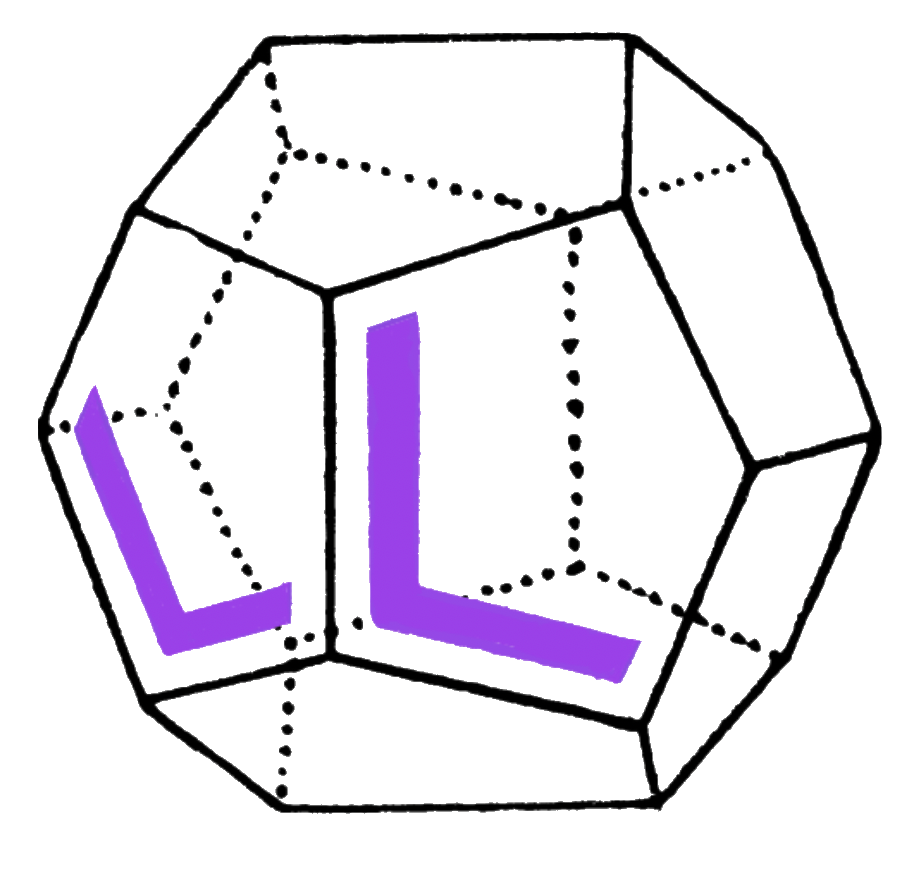
\includegraphics[width=2cm,height=2cm]{ll.png}}

    }}

\AddToShipoutPicture*
  {\put(470,767){
    \href{https://github.com/linlib/ThreeWhiteheadTheorems/StringDiagramGenerator.py}{\texttt{.py file}}
  }}

\AddToShipoutPicture*
  {\put(470,752){
    \href{https://github.com/linlib/ThreeWhiteheadTheorems/ThreeWhiteheadTheorems.tex}{\texttt{.tex file}}\\

  }}


\AddToShipoutPicture*
  {\put(470,737){

    \href{http://linearlibrary.net/ThreeWhiteheadTheorems/October19th.pdf}{\texttt{.pdf file}}\\

  }}

  \AddToShipoutPicture*
  {\put(470,722){
    \href{https://github.com/linlib/ThreeWhiteheadTheorems/ThreeWhiteheadTheorems.lean}{\texttt{.lean file}}

  }}

\ \\

%LEAN: 
\begin{center}
\begin{tcolorbox}[width=5.8in,colback={white},coltitle=white]
\begin{center}
\ \\
\scalebox{3}{\texttt{𝕋𝕙𝕣𝕖𝕖 𝕎𝕙𝕚𝕥𝕖𝕙𝕖𝕒𝕕 𝕋𝕙𝕖𝕠𝕣𝕖𝕞𝕤}}\\
\ \\
\scalebox{3}{\texttt{𝕒𝕟𝕕}}\\
\ \\
\scalebox{3}{\texttt{𝕋𝕙𝕣𝕖𝕖 ℙ𝕦𝕡𝕡𝕖 𝕊𝕖𝕢𝕦𝕖𝕟𝕔𝕖𝕤}}\\
\ \\
\end{center}
\end{tcolorbox}
\end{center}
\ \\
{\footnotesize
\begin{center}
\scalebox{1.1}{
\begin{tabular}{|| l | l || l | l | l | l || l | l || l | l | l | l || } 
\hline
$\texttt{IntCat}$ & \texttt{D⃗(}∞\texttt{-Cat)} & Ω⃗ & P⃗ & B⃗ & E⃗ & $\texttt{IntPrShf}$ & \texttt{D⃗(}∞\texttt{-Cat/C)} & ω⃗ &  p⃗ & b⃗ & e⃗\\
\hline
$\texttt{IntGrpd}$ & \texttt{D⃡(}∞\texttt{-Grpd)} & Ω⃡ & P⃡ & B⃡ & E⃡ & $\texttt{IntAct}$ & \texttt{D⃡(}∞\texttt{-Grpd/G)} & ω⃡ & p⃡ & b⃡ & e⃡\\
 \hline
$\texttt{IntGrp}$ & \texttt{D(}∞\texttt{-Grpd₀)} & Ω & P & B & E & $\texttt{IntAct₀}$ & \texttt{D(}∞\texttt{-Grpd₀/G₀)} & ω & p & b & e\\
 \hline
\end{tabular}}
\end{center}}
\ \\
%LEAN: 
\begin{center}
\begin{tcolorbox}[width=6in,colback={white}]
\begin{center}
\scalebox{0.9}{∀(C:D⃗(∞-Cat)),∀(D:D⃗(∞-Cat)),∀(F:C ⭢ D),∀(G:C ⭢ D),(∀(n:Nat),(π⃗ₙ F = π⃗ₙ G)) → F = G}\\
\ \\
\scalebox{0.9}{∀(X:D⃡(∞-Grpd)),∀(Y:D⃡(∞-Grpd)),∀(f:X ⭢ Y),∀(g:X ⭢ Y),(∀(n:Nat),(π⃡ₙ f = π⃡ₙ g)) → f = g}\\
\ \\
\scalebox{0.9}{∀(X:D(∞-Grpd₀)),∀(Y:D(∞-Grpd₀)),∀(f:X ⭢ Y),∀(g:X ⭢ Y),(∀(n:Nat),(πₙ f = πₙ g)) → f = g}\\
\ \\
\scalebox{0.9}{$\cdots$ ⭢ π⃗₁.obj C ⭢ π⃗₁.obj D $\circlearrowright$ π⃗₀.obj ((𝟙 C) • ((ω⃗.hom (𝟙 D)).hom f) ) ⭢ (π⃗₀.obj C) ⭢ (π⃗₀.obj D)}\\
\ \\
\scalebox{0.9}{$\cdots$ ⭢ π⃡₁.obj E ⭢ π⃡₁.obj B $\circlearrowright$ π⃡₀.obj ((𝟙 B) • ((ω⃡.hom (𝟙 C)).hom f) ) ⭢ (π⃡₀.obj E) ⭢ (π⃡₀.obj B)}\\
\ \\
\scalebox{0.9}{$\cdots$ ⭢ π₁.obj E₀ ⭢ π₁.obj B₀ ⭢ π₀.obj ((𝟙 B₀) • ((ω.hom (𝟙 B₀)).hom f)) ⭢ π₀.obj (E₀) ⭢ π₀.obj(B₀)}\\
\ \\
\end{center}
\end{tcolorbox}
\end{center}

%LEAN: 
\begin{center}
\begin{tcolorbox}[width=4.13in,colback={white},coltitle=white]
\scalebox{2}{𝔼𛲔 𝔻𝕖𝕒𝕟 𝕐𝕠𝕦𝕟𝕘 𝕒𝕟𝕕 𝕁𝕚𝕒𝕫𝕙𝕖𝕟 𝕏𝕚𝕒}
\end{tcolorbox}
\end{center}


\begin{center}
\texttt{Plans to prove three variations of the}\\
\texttt{Whitehead theorem and the exactness of}\\
\texttt{three variations of the Puppe sequence of}\\
\texttt{homotopy groups for based ∞-groupoids}\\
\texttt{in Lean 4, with extensive use of Mathlib's}\\
\texttt{categories, functors, natural transformations,}\\
\texttt{Eilenberg-Moore theory, pullbacks, products,}\\
\texttt{simplices, cube, boundary of simplex,}\\
\texttt{boundary of cube, horns, inner horns,}\\
\texttt{}
\end{center}


\thispagestyle{empty}


\newpage


\begin{center}

\pagecolor{white}
\color{black}




\end{center}

\thispagestyle{empty}




\newpage
\pagecolor{white}
\color{black}
\ \\
\ \\
\thispagestyle{empty}
\begin{center}
Copyright\ \textcopyright \ October 19th 2023 Elliot Dean Young.\ All rights reserved.\\
\end{center}
\large %%%%%%%% HERE IS THE large LARGE size textsize set text size
\newpage 
\ \\
\ \\
\ \\
\ \\
\ \\
\ \\
\ \\
\ \\
\ \\
\ \\
\ \\
\thispagestyle{empty}
 
\newpage



\newpage

\ \\
\ \\
\ \\
\ \\
\ \\
\ \\
\ \\
\ \\
\ \\
\ \\
\ \\

We wish to acknowledge the collaborative efforts of E. Dean Young and Jiazhen Xia (夏家桢). The first author initially formulated the extensive outline and twelve goals presented in this research, and both made valuable contributions refining, extending, and implementing them.\\

\iffalse
\begin{center}
\begin{tcolorbox}[width=4in,colback={White},title={},colbacktitle=White,coltitle=black]
\texttt{Hundreds of years into the future, we look back on those who stood against the conservative extension ℝ → ℂ with a clarity that assures us they had nothing to fear...}
\end{tcolorbox}
\end{center}
\fi


\newpage

\begin{enumerate}
\item Categories (see Mathlib's $\texttt{Category X}$ here; these can be bundled into $\texttt{category}$)
\item Functors (see Mathlib's $\texttt{Functor C D}$ here; these can be bundled into $\texttt{functor}$)
\item NaturalTransformation (see Mathlib's $\texttt{NaturalTransform F G}$ here; these can be bundled into $\texttt{natural\_transform}$)
\item Equations (see Mathlib's $\texttt{NatExt}$ here; these are related to our $\texttt{equation}$)
\end{enumerate}

\begin{enumerate}
\item IntCat : Cat → Cat 
\item IntPrShf : (X : Cat) → (C : (IntCat X)) → Cat
\item IntGrpd : Cat → Cat
\item IntAct : (X : Cat) → (G : (IntGrpd X)) → Cat
\item IntGrp : Cat → Cat
\item IntAct₀ : (X : Cat) → (G₀ : (IntGrp X)) → Cat
\end{enumerate} 

Below is a complete list of the symbols we define and the theorems we define and prove:

\iffalse
{
\footnotesize
\begin{longtable}{|| l | l | l | l ||} 
\hline
$\texttt{Symbol}$ & $\texttt{Name}$ & \texttt{Type}& \texttt{Information} &  $\texttt{Description}$ \\
\hline
\hline
Ω⃗ & \scalebox{0.6}{Monadic endofunctor} & Monadic endofunctor of  & \scalebox{}{Representable by Δ¹} \\
\hline
P⃗ & \scalebox{0.6}{} & & \\
\hline
B⃗ & \scalebox{0.6}{} & & \\
\hline
E⃗ & & & \\
\hline
ω⃗ &  & & \\
\hline
p⃗ &  \scalebox{0.6}{Remembrant directed derived directed homotopy pullback} & & \\
\hline
b⃗ &  & & \\
\hline
e⃗ &  & & \\
\hline
Ω⃡ &  \scalebox{0.6}{Path space} & &\\
\hline
P⃡ & & & \\
\hline
B⃡ & & & \\
\hline
E⃡ & & & \\
\hline 
ω⃡ & & & \\
\hline
p⃡ & & & \\
\hline
b⃡ & & & \\
\hline
e⃡ & & & \\
\hline
Ω & \scalebox{0.6}{Loop space}  & & \\
\hline
P & \scalebox{0.6}{Remembrant derived loop space} & & \\
\hline
B & \scalebox{0.6}{Classifying space} & & \\
\hline
E & \scalebox{0.6}{Classifying space} & & \\
\hline
ω &  & & \\
\hline
p & \scalebox{0.6}{Remembrant derived homotopy fiber} & & \\
\hline
b &  & & \\
\hline
e &  & &\\
\hline
\hline
π⃗₀ & \texttt{Whitehead Theorem (a)} & & \\
\hline
π⃡₀ & \texttt{Whitehead Theorem (b)} & & \\
\hline
π₀ & \texttt{Whitehead Theorem ()} & & \\
\hline
ρ⃗ & \scalebox{0.6}{Quotient of an internal $C$-presheaf} & & \\
\hline
ρ⃡ & \scalebox{0.6}{Quotient of an internal $G$-presheaf} & & \\
\hline
ρ & \scalebox{0.6}{Quotient of an internal $G₀$-action} & & \\
\hline
\end{longtable}
}
\fi


\iffalse
\texttt{repl} & & &\\
\hline 
\texttt{∞} & & & \\
\hline 
\texttt{*} & &  &\\
\hline
\texttt{⊥} & & & \\
\fi




\newpage



\newpage
\section{Contents}

{
\footnotesize
\begin{longtable}{|| l || l ||} 
\hline
\multicolumn{1}{||c||}{$\texttt{Section}$} & \multicolumn{1}{|c||}{$\texttt{Description}$} \\
\hline
\hline
Unfinished & \\
\hline
Contents & \\
\hline
Unicode & \\
\hline
Introduction & \\
\hline \hline
\multicolumn{2}{||c||}{\texttt{Chapter 1: Mathlib's Category Theory Library}} \\
\hline \hline
$\texttt{Category, Functor, NaturalTransform}$ & Mathlib's categories, functors, and natural transformations \\
\hline
$\texttt{Bicategory.Cat}$ & Mathlib's bicategory of categories \\
 \hline
⊣,⇄,⇆,ॱ,𛲔 & Mathlib's adjunctions, monads, and comonads\\
  \hline
!,¡,?,¿,ꜝ,ꜞ & Mathlib's Eilenberg Moore theory\\
   \hline
× & Mathlib's pullbacks and products\\
\hline
$\texttt{SSet, Δⁿ, Λ???}$ & Mathlib's simplicial sets, simplices, and horns\\
\hline \hline
 \multicolumn{2}{||c||}{\texttt{PART I: } ∞-Categories} \\
\hline \hline
\multicolumn{2}{||c||}{\texttt{Chapter 2: }∞\texttt{-Cat}} \\
\hline \hline
D⃗(∞-Cat) & The derived category of ∞-categories \\
\hline
D⃗(∞-Cat⁄C) & The derived category of ∞-categories over C \\
\hline
Ω⃗ : ∞-Cat ⭢ ∞-Cat & The directed path space functor \\
 \hline 
ω⃗ f : ∞-Cat⁄D ⭢ ∞-Cat/C & The directed homotopy pullback functor\\
 \hline 
π⃗ₙ : ∞-Cat ⭢ Set & The connected components functors\\
 \hline \hline
 \multicolumn{2}{||c||}{\texttt{Chapter 3: }The Whitehead Theorem for ∞-Categories} \\
\hline \hline
REP for ∞-categories & The cofibrant replacement functor for ∞-categories\\
\hline
HEP for ∞-categories & The directed homotopy extension property\\
\hline 
Whitehead theorem (a) & A map $\texttt{F : D(}$∞$\texttt{-Cat).Hom E B}$ is determined by $\texttt{λ(n:Nat),}$π⃗ₙ$\texttt{F}$.\\
\hline \hline
\multicolumn{2}{||c||}{\texttt{Chapter 4: Internal Categories and Internal Sheaves}} \\
\hline \hline
 $\texttt{IntCat Γ C}$   & The category of internal categories \\
 \hline
 $\texttt{IntPrShf Γ C X}$   & The category of internal presheaves \\
 \hline
  The internal category principal & \texttt{f ×\_(B) f} forms a component of an internal category \\
 \hline
 The internal presheaf principal & \texttt{f ×\_(B) g} forms a component of an internal presheaf \\
 \hline
P⃗ : D(∞-Cat) ⭢ IntCat D(∞-Cat)  & The (remembrant derived) directed path space functor \\
 \hline 
p⃗ C : D(∞-Cat⁄C) ⭢ IntPrShf D(∞-Cat⁄C) & The (remembrant derived) directed homotopy pullback functor\\
 \hline \hline
 \multicolumn{2}{||c||}{\texttt{Chapter 5: }The Puppe Sequence for ∞-Categories} \\
\hline \hline
The Puppe sequence & \scalebox{0.8}{$\cdots$ ⭢ π⃗₁(C) ⭢ π⃗₁(D) $\circlearrowright$ π⃗₀(ω⃗ (𝟙 D) f) ⭢ π⃗₀(C) ⭢ π⃗₀(D)}  \\
\hline \hline
\multicolumn{2}{||c||}{\texttt{Chapter 6: }The Categorical Fixed Point Principals} \\
\hline \hline
The internal category principal & \texttt{D(}∞\texttt{-Cat)} is equivalent to deloopable internal categories in itself \\
\hline
The internal sheaf principal & \texttt{D(}∞\texttt{-Cat⁄C)} is equivalent to deloopable internal presheaves in itself \\
 \hline \hline
 \multicolumn{2}{||c||}{\texttt{PART II: } ∞-Groupoids} \\
\hline \hline 
\multicolumn{2}{||c||}{\texttt{Chapter 7: }∞\texttt{-Grpd}}\\
\hline \hline
D⃡(∞-Grpd) & The derived category of ∞-groupoids \\
\hline
D⃡(∞-Grpd/X) & The derived category of ∞-groupoids over X \\
\hline
Ω⃡ : ∞-Grpd ⭢ ∞-Grpd & The directed path space functor \\
 \hline 
ω⃡ f : ∞-Grpd⁄D ⭢ ∞-Grpd/C & The directed homotopy pullback functor\\
 \hline 
π⃡ₙ : ∞-Grpd ⭢ Set & The connected components functors\\
 \hline \hline
 \multicolumn{2}{||c||}{\texttt{Chapter 8: }The Whitehead Theorem for ∞-Groupoids} \\
\hline \hline
REP for ∞-groupoids & The cofibrant replacement functor for ∞-groupoids\\
\hline
HEP for ∞-groupoids & The homotopy extension property\\
\hline
Whitehead theorem (b) & A map $\texttt{F : D(}$∞$\texttt{-Grpd).Hom E B}$ is determined by $\texttt{λ(n:Nat),}$π⃡ₙ
$\texttt{F}$. \\
\hline \hline
\multicolumn{2}{||c||}{\texttt{Chapter 9: }Internal Groupoids and their Internal Sheaves} \\
\hline \hline
 $\texttt{IntGrpd Γ}$   & The category of internal groupoids in Γ \\
 \hline
 $\texttt{IntAct Γ G}$ & The category of internal G-actions in Γ \\
 \hline
  The internal groupoid principal & \texttt{f ×\_(B) f} forms an internal groupoid\\
 \hline
 The internal groupoid action principal & \texttt{f ×\_(B) g} forms an internal groupoid action \\
 \hline
 P⃡ & The (remembrant derived) path space functor \\ 
\hline
 p⃡ C & The (remembrant derived) homotopy pullback functor  \\
 \hline \hline
 \multicolumn{2}{||c||}{\texttt{Chapter 10: }The Puppe Sequence for ∞-Groupoids} \\
\hline \hline
The Puppe sequence & \scalebox{0.8}{$\cdots$ ⭢ π⃡₁(E) ⭢ π⃡₁(B) $\circlearrowright$ π⃡₀(ω⃡ (𝟙 C) f) ⭢ π⃡₀(E) ⭢ π⃡₀(B)} \\
\hline \hline
\multicolumn{2}{||c||}{\texttt{Chapter 11: }The Groupoid Fixed Point Principals} \\
\hline \hline
The internal groupoid delooping principal & \texttt{D(}∞\texttt{-Grpd)} is deloopable internal categories in itself \\
\hline
The internal groupoid action delooping principal & \texttt{D(}∞\texttt{-Grpd⁄C)} is deloopable internal groupoid actions in itself \\
\hline \hline
 \multicolumn{2}{||c||}{\texttt{PART III: } Based Connected ∞-Groupoids} \\
\hline \hline
\multicolumn{2}{||c||}{\texttt{Chapter 12: }Based Connected ∞-Groupoids} \\
\hline \hline
D(∞-Grpd₀) & The derived category of based connected ∞-groupoids \\
\hline
D(∞-Grpd₀/X₀) & The derived category of based connected ∞-groupoids over X₀. \\
\hline
Ω : ∞-Grpd₀ ⭢ ∞-Grpd & The loop space functor \\
\hline
ω f : D(∞-Grpd/D₀) ⭢ D(∞-Grpd⁄C₀) & The homotopy fiber\\
 \hline 
πₙ : ∞-Grpd₀ ⭢ Set & The connected components functors\\
 \hline \hline
  \multicolumn{2}{||c||}{\texttt{Chapter 13: }The Whitehead Theorem for Based Connected ∞-Groupoids} \\
\hline \hline
REP for based connected ∞-groupoids & The replacement functor on ∞$\texttt{-Grpd}$₀ \\
\hline
HEP for based connected ∞-groupoids & The homotopy extension property for ∞$\texttt{-Grpd}$₀\\
 \hline 
Whitehead theorem (c) & A map $\texttt{F : D(}$∞$\texttt{-Grpd₀).Hom E₀ B₀}$ is determined by $\texttt{λ(n:Nat),πₙ F}$. \\
\hline \hline
 \multicolumn{2}{||c||}{\texttt{Chapter 14: }Internal Groups} \\
\hline \hline
 $\texttt{IntGrp Γ}$   & The category of internal groups in Γ  \\
 \hline
 $\texttt{IntAct₀ Γ G₀}$ & The category of internal G₀-actions in Γ   \\
 \hline
 The internal group principal & Ω X forms an internal group in D(∞-Grpd) \\
 \hline
 The internal group action principal & ω f forms an internal group action in D(∞-Grpd⁄G₀) \\
 \hline
 P & The (remembrant derived) path space functor \\ 
\hline
 p G₀ & The (remembrant derived) homotopy fiber  \\
\hline \hline
 \multicolumn{2}{||c||}{\texttt{Chapter 15: }The Puppe Sequence for Based Connected ∞-Groupoids} \\
\hline \hline
The Puppe sequence & \scalebox{0.8}{$\cdots$ ⭢ π₁(E₀) ⭢ π₁(B₀) ⭢ π₀(ω (𝟙 X₀)) ⭢ π₀(E₀) ⭢ π₀(B₀)}  \\
\hline \hline
\multicolumn{2}{||c||}{\texttt{Chapter 16: }The Categorical Equivalences for Based Connected ∞-Groupoids} \\
\hline \hline
The internal group delooping principal & \texttt{D(}∞\texttt{-Grpd₀)} and internal groups in based spaces \\
\hline
The internal group action delooping principal & \texttt{D(}∞\texttt{-Grpd}₀\texttt{/G}₀\texttt{)} and internal ΩG₀-actions in \texttt{D(}∞\texttt{-Grpd₀⁄G₀)} \\
 \hline 
\end{longtable}
}

\iffalse
\multicolumn{2}{||c||}{\texttt{Chapter 2: Straightening Systems}} \\
\hline \hline
$\texttt{s\_(Γ) f} $ & The directed homotopy pullback adjunction \\ 
\hline
$\texttt{S\_(Γ) f} $ & The directed path-space adjunction \\ 
\hline
$\texttt{*\_(Γ)}$  & The point \\ 
\hline
$\texttt{∞\_(Γ)}$ & The universe object \\ 
\hline
$\texttt{⊥\_(Γ)}$ & The overobject classifier  \\
\hline
$\texttt{χ\_(Γ)}$ & The characteristic morphism \\
\hline \hline
\multicolumn{2}{||c||}{\texttt{Chapter 3: Sets as a pullback system}} \\
\hline\hline
𝕊𝕖𝕥 & The pullback system of sets \\
\hline \hline
\fi



\newpage
\section{Introduction}

The {\bf main goal} of this text is {\bf to prove the Whitehead theorem concerning based connected attaching-map-complexes for the case of a homotopy category of \texttt{SSet} with a lifting condition}. The book ``Galois theories" by Borceux and Janelidze deserves special mention as an inspiration for the present project. That book details how to think about Galois theory using internal groupoids, internal G-presheaves, monadicity, comonadicity, and the constructions involved in Eilenberg-Moore theory.\\

Here are the three Whitehead Theorems which form our main three goals:

\begin{enumerate}[(a)]
\item (The Whitehead theorem for ∞-categories) ∀(E:D⃗(∞-Cat)),∀(B:D⃗(∞-Cat)),∀(F:E ⭢ B),∀(G:E ⭢ B),(∀(n:Nat),(π⃗ₙ F = π⃗ₙ G)) → F = G, where π⃗ₙ is notation for π⃗ n.
\item (The Whitehead theorem for ∞-groupoids) ∀(E:D⃡(∞-Grpd)),∀(B:D⃡(∞-Grpd)),∀(F:E ⭢ B),∀(G:E ⭢ B),(∀(n:Nat),(π⃡ₙ F = π⃡ₙ G)) → F = G, where π⃡ₙ is notation for π⃡ n.
\item (The Whitehead theorem for based connected ∞-groupoids) ∀(E:D(∞-Grpd₀)),∀(B:D(∞-Grpd₀)),∀(F:E ⭢ B),∀(G:E ⭢ B),(∀(n:Nat),(πₙ F = πₙ G)) → F = G, where πₙ is notation for π n.
\end{enumerate}

\iffalse
We will be using two different models of ∞-Grpd, a model of ∞-Cat, a model of D(∞-Cat) (based on REP and HEP detailed in chapter 3), and model of 𝓓(∞-Cat/C) in which Whitehead theorem (a) is forced. This is perhaps unimpressive, and also leads us to thinking about replacement as an endofunctor $\texttt{repl} : \texttt{Functor}$∞$\texttt{-Cat}$ ∞$\texttt{-Cat}$, which is involved in both the statement and proof of REP, and which is designed in a way such that HEP holds.\\
\fi

\iffalse
Forcing the Puppe sequence to hold  D(∞-Cat⁄C)
\fi

We will use the following models in the theorem above:

\begin{enumerate}[(i)]
\item ∞-Cat is the category of quasicategories.
\item ∞-Grpd is the category of simplicial sets with the Kan lifting condition.
\item ∞-Grpd₀ is the category of based connected simplicial sets with the Kan lifting condition.
\end{enumerate}

The operations require great care in their definition. The existence of a base point makes πₙ relatively easy to define, while π⃗ₙ and π⃡ₙ require careful consideration and get much larger by comparison:

\begin{enumerate}[(i)]
\item π⃗ₙ : ∞-Cat ⭢ Set
\item π⃡ₙ : ∞-Grpd ⭢ Set
\item πₙ : ∞-Grpd₀ ⭢ Set
\end{enumerate}

we also form

\begin{enumerate}[(i)]
\item D⃗(π⃗ₙ) : D⃗(∞-Cat) ⭢ D⃗(Set) ≃ Set
\item D⃡(π⃡ₙ) : D⃡(∞-Grpd) ⭢ D⃡(Set) ≃ Set
\item D(πₙ) : D(∞-Grpd₀) ⭢ D(Set) ≃ Set
\end{enumerate}

and

\begin{enumerate}
\item Ω⃗ : ∞-Cat ⭢ ∞-Cat is the internal hom functor [Δ¹,-] (directed path space)
\item Ω⃡ : ∞-Grpd ⭢ ∞-Grpd is the internal hom functor [I,-] (path space)
\item Ω is the loop space functor
\end{enumerate}

The first of the Whitehead theorems, (a), is the most abstract. The third, (c), is the one from Whitehead's original papers. The second forms a nice intermediate between the two.\\



The choice of quasicategories gives nice integration with Mathlib's existing features (though technically only the inner horns and simplices are defined, not even the category of quasicategories itself), a possible benefit over a more ``synthetic" approach based on forcing the three Whitehead theorems and three Puppe sequences at the outset (along with the functors, natural isomorphisms, and equations in the first several pages). \\

The main technical feature in the proofs of these theorems concerns a lifting property which successively lifts a homotopy${}^{***}$ along a single attachment of Δⁿ along its boundary ∂Δⁿ. A homotopy h : ∂Δⁿ × Δ¹ ⭢ Y between f, g : ∂Δⁿ ⭢ Y extends to a map H : Δⁿ × Δ¹ ⭢ Y. H(-,1) and g match on ∂Δⁿ, producing a map f : X ⭢ Y, where X consists of two copies of Δⁿ glued together at the boundary. Consider a space X' formed as a quotient of Δⁿ × Δ¹ by ∂Δⁿ × Δ¹. There is a map φ : X ⭢ X'. An induction hypothesis on f and g involving πₙ ensures that the aparent map X ⭢ Y lifts along φ, producing a map from Δⁿ × Δ¹ which is constant on ∂Δⁿ × Δ¹. Stacking this on top of H can be done using an isomorphism between Δ¹ and Δ¹ glued with itself along different endpoints. Altogether this produces a homotopy between f and g.\\

${}^{***}$ Note that a homotopy here is to do with the directed derived category of an overcategory D(∞-Cat⁄C), and it consists of really a sequence of compatible directed homotopies with the odd morphisms formed from reversed copies of Δ¹. Really we have two such categories, one of which consists of formal words, and another which involves ∞-categories and ∞-functors in the image of $\texttt{repl}$) \\

\iffalse
Here are two fairly basic observations about the first two structures:\\

\begin{enumerate}
\item Define and inhabit the $\texttt{internal\_category\_principal : Type}$. This principal results from reflecting on how the pullback of f : E ⭢ B with itself forms the morphism component of an internal category for which we write P⃗ f.
\item Define and inhabit the $\texttt{internal\_presheaf\_principal : Type}$. This principal results from refecting on how the pullback of f : E ⭢ B with g : F ⭢ B forms a component of an internal (P⃗ f)-presheaf for which we write ω⃗ f g.
\end{enumerate}

The functors ω⃗ and Ω⃗, along with various Mathlib constructions from Eilenberg-Moore theory, can be used to construct these functors (which feature ).\\
\fi

Using the mentioned categories, we will define three different kinds of derived category:\\

\begin{enumerate}
\item D(∞-Cat) : Cat (the directed derived category of ∞-categories)
\item D(∞-Grpd) : Cat (the derived category of ∞-groupoids)
\item D(∞-Grpd₀) : Cat (the derived category of based ∞-groupoids)
\end{enumerate}

These are formed by identifying those morphisms (∞-functors) between which there is a natural transformation.\\

We also create a second kind of category, one for each of the objects in the respective categories above:

\begin{enumerate}
\item For C : D(∞-Cat), a category D(∞-Cat/C) : Cat
\item For G : D(∞-Grpd), a category D(∞-Grpd/G) : Cat
\item For G₀ : D(∞-Grpd₀), a category D(∞-Grpd₀/G₀) : Cat
\end{enumerate}

For the model built on simplicial sets, Ω⃗ will be representable by Δ¹ with respect to an internal hom, and Ω⃡ will be representable by a model of the unit interval I := [0,1].\\

The six mentioned internal structures are related to six functors:

\begin{enumerate}[(I)]
\item Ω⃗ : ∞-Cat ⭢ ∞-Cat (notation for the directed path space functor, related to [Δ¹,-]). D(Ω⃗) factors through internal categories in D(∞-Cat) by a categorical equivalence D(∞-Cat) ≅ IntCat D(∞-Cat) (internal categories in D(∞-Cat))
\item ω⃗ (𝟙 C) : ∞-Cat/C ⭢ ∞-Cat/C, the derived directed homotopy pullback with 𝟙 C. D(ω⃗ (𝟙 C)) factors through a categorical equivalence between D(∞-Cat/C) and internal P⃗C-presheaves in D(∞-Cat/C).
\item Ω⃡ : ∞-Grpd ⭢ ∞-Grpd (notation for the path space functor [I,-]), the derived homotopy pullback of an ∞-groupoid with itself. D(Ω⃡) factors through a categorical equivalence between D(∞-Grpd) and internal groupoids in D(∞-Grpd)
\item ω⃡ (𝟙 X) : ∞-Grpd/X ⭢ ∞-Grpd/X, the derived homotopy pullback with 𝟙 X. D(ω⃡ (𝟙 X)) factors through internal P⃡X
\item Ω : ∞-Grpd₀ ⭢ ∞-Grpd₀, the loop space functor. D(Ω) factors through a categorical equivalence between D(∞-Grpd₀) and internal groups in D(∞-Grpd₀) (the loop space functor on connected based ∞-groupoids)
\item ω (𝟙 X) : ∞-Grpd₀/X₀ ⭢ ∞-Grpd₀/X₀, the homotopy pullback with the base of X₀. D(ω (𝟙 X)) factors through internal PX₀-actions in based connected spaces over X₀.
\end{enumerate}

(v) in the above is shown \href{https://mathoverflow.net/questions/128883/why-omega-x-and-bg-are-adjoint-functors}{here} and (vi) in the above is shown in a typical treatment of $G$-principal bundles.\\

The functors ω⃗ (𝟙 C), ω⃡ (𝟙 X), and ω (𝟙 C) in the above ensue from a more general construction:\\

\begin{enumerate}
\item For C, D : D(∞-Cat), and f : C ⭢ D, ω⃗ f : D(∞-Cat/D) ⭢ D(∞-Cat/C)   (derived directed homotopy pullback)
\item For B, E : D(∞-Grpd), and f : E ⭢ B, ω⃡ f : D(∞-Grpd/B) ⭢ D(∞-Grpd/E) (derived homotopy pullback)
\item For B₀, E₀ : D(∞-Grpd₀), and f : E₀ ⭢ B₀, ω f : D(∞-Grpd₀/B₀) ⭢ D(∞-Grpd₀/E₀) (homotopy pullback with the base)
\end{enumerate}

These six factored functors P⃗ , P⃡ , P : D(∞-Grpd₀), p⃗ (𝟙 C), p⃡ (𝟙 X), p are each fully faithful and produce categorical equivalences; we later construct functors B⃗, B⃡, B, b⃗, b⃡, b defined on the essential image of these six, which are inverse to them up to natural isomorphism.\\

We obtain six categorical equivalences witnessed by these twelve functors (along with twelve natural isomorphisms). Here are the types of P⃗ , P⃡ , P : D(∞-Grpd₀), p⃗ (𝟙 C), p⃡ (𝟙 X), p:

\begin{enumerate}
\item The directed path space, the path space, and loop space form components of the functors P⃗, P⃡, and P, which are valued in internal categories, internal groupoids, and internal groups respectively.
\begin{enumerate}
\item P⃗ : D(∞-Cat) ⭢ Cat D(∞-Cat)
\item P⃡ : D(∞-Grpd) ⭢ Grpd D(∞-Grpd)
\item P : D(∞-Grpd₀) ⭢ Grp D(∞-Grpd) (see \href{https://mathoverflow.net/questions/128883/why-omega-x-and-bg-are-adjoint-functors}{here})
\end{enumerate}
\item The directed homotopy pullback, the homotopy pullback, and the homotopy pullback with the base form components of the functors Alg(Mon(ω⃗)), Alg(Mon(ω⃡)), and Alg(Mon(p)), respectively. 
\begin{enumerate}
\item p⃗ (𝟙 C) : D(∞-Cat⁄C) ⭢ IntPrShf D(∞-Cat⁄C) Ω⃗C 
\item p⃡ (𝟙 X) : D(∞-Grpd⁄X) ⭢ IntAct D(∞-Grpd⁄X) Ω⃡X
\item p (𝟙 X₀) : D(∞-Grpd₀⁄X₀) ⭢ IntAct₀ D(∞-Grpd₀⁄X₀) ΩX₀
\end{enumerate}
\end{enumerate}

Above, the functors P⃗, P⃡, P, p⃗, p⃡, and p feature Ω⃗, Ω⃡, Ω, ω⃗, ω⃡, and ω in their components, and can be related to them using constructions from Eilenberg-Moore theory.\\

These six new functors combine with the functors below to form categorical equivalences:\\

\begin{enumerate}
\item The directed homotopy colimit of a point with an internal category in D(∞-Cat) as a diagram, the homotopy colimit of a constant functor with an internal internal group as a diagram
\begin{enumerate}
\item B⃗ : essential_image P⃗ ⭢ D(∞-Cat)
\item B⃡ : essential_image P⃡ ⭢ D(∞-Grpd)
\item B : essential_image P ⭢ D(∞-Grpd₀) (see \href{https://mathoverflow.net/questions/128883/why-omega-x-and-bg-are-adjoint-functors}{here})
\end{enumerate}
\item The clutching functors are inverse to the above functors up to natural isomorphism:
\begin{enumerate}
\item b⃗ : essential_image p⃗ ⭢ D(∞-Cat⁄C)
\item b⃡ : essential_image p⃡ ⭢ D(∞-Cat⁄C)
\item b : essential_image p ⭢ D(∞-Grpd₀⁄X₀) 
\end{enumerate}
\end{enumerate}

\iffalse
The essential images of B and b are...
\if

As mentioned, we will show six categorical equivalences featuring these:

\begin{enumerate}
\item P⃗ • B⃗ ≅ 𝟙 (IntCat D(∞-Cat)) and B⃗ • P⃗ ≅ 𝟙 D(∞-Cat)
\item P⃡ • B⃡ ≅ 𝟙 (IntGrpd D(∞-Grpd)) and B⃡ • P⃡ ≅ 𝟙 D(∞-Grpd)
\item P • B ≅ 𝟙 (IntGrp D(∞-Grpd₀)) and B • P ≅ 𝟙 D(∞-Grpd₀) (see \href{https://mathoverflow.net/questions/128883/why-omega-x-and-bg-are-adjoint-functors}{here})
\item p⃗ • b⃗ ≅ 𝟙 (IntPrShf D(∞-Cat⁄C) P⃗C) and b⃗ • p⃗ ≅ 𝟙 D(∞-Cat⁄C)
\item p⃡ • b⃡ ≅ 𝟙 (IntAct D(∞-Cat⁄C) P⃡X) and b⃡ • p⃡ ≅ 𝟙 D(∞-Cat⁄C) 
\item p • b ≅ 𝟙 (IntAct₀ D(∞-Grpd₀⁄X₀) PX₀) and b • p ≅ 𝟙 D(∞-Grpd₀⁄X₀) (see \href{https://en.wikipedia.org/wiki/Principal_bundle}{here})
\end{enumerate}

We will make extensive use of Mathlib's \href{https://leanprover-community.github.io/mathlib4_docs/Mathlib/CategoryTheory/Category/Cat.html#CategoryTheory.Cat.bicategory}{bicategory of categories} and material on \href{https://github.com/leanprover-community/mathlib4/blob/bd3e369b6f82c874de0f318c71d7e0595f8a3aa4//Mathlib/AlgebraicTopology/SimplicialSet.lean#L47-L48}{simplicial sets}. We further use Mathlib's pullbacks and \href{https://github.com/leanprover-community/mathlib4/blob/bd3e369b6f82c874de0f318c71d7e0595f8a3aa4/Mathlib/CategoryTheory/Products/Basic.lean}{categorical products}, as well as their \href{https://github.com/leanprover-community/mathlib4/blob/bd3e369b6f82c874de0f318c71d7e0595f8a3aa4/Mathlib/CategoryTheory/Monad/Algebra.lean}{Eilenberg-Moore theory constructions}. I'd like to extend my appreciation to Scott Morison, Eric Wieser, Floris Van Doorne, and all the contributors who have put their efforts into creating these robust features for Mathlib 4.\\

Altogether, the project gets the following ``periodic table" of 24 functors featured on the front cover:\\

{\footnotesize
\begin{center}
\scalebox{1.5}{
\begin{tabular}{|| l || l | l | l | l || l || l | l | l | l || } 
\hline
\texttt{D(}∞\texttt{-Cat)} & Ω⃗ & P⃗ & B⃗ & E⃗ & \texttt{D(}∞\texttt{-Cat/C)} & ω⃗ & b⃗ & p⃗  & e⃗ \\
\hline
\texttt{D(}∞\texttt{-Grpd)} & Ω⃡ & P⃡ & B⃡ & E⃡ & \texttt{D(}∞\texttt{-Grpd/G)} & ω⃡ & b⃡ & p⃡ & e⃡ \\
 \hline
\texttt{D(}∞\texttt{-Grpd₀)} & Ω & P & B & E & \texttt{D(}∞\texttt{-Grpd₀/G₀)} & ω & b & p & e \\
 \hline
\end{tabular}}
\end{center}}

Here are the names of the symbols featured above:

{\footnotesize
\begin{center}
\begin{tabular}{|| l | l | l | l || } 
\hline
\hline
\texttt{Deductive} & \texttt{Remembrant} & \texttt{Delooping} & \texttt{Free} \\
\hline
\hline
Ω⃗ \scalebox{0.7}{(Directed path space)} & P⃗ \scalebox{0.7}{(Remembrant derived directed path space)} & B⃗ \scalebox{0.7}{(Classifying space for internal categories)}  & E⃗ \\
\hline
Ω⃡ \scalebox{0.7}{(Path space)} & P⃡ \scalebox{0.7}{(Remembrant derived path space)} & B⃡ \scalebox{0.7}{(Classifying space for internal groupoids)} & E⃡  \\
 \hline
Ω \scalebox{0.7}{(Loop space)} & P \scalebox{0.7}{(Remembrant derived loop space)} & B \scalebox{0.7}{(Classifying space for internal groups)} & E \\
 \hline
 \hline
ω⃗ \scalebox{0.7}{(Directed homotopy pullback)} & p⃗ \scalebox{0.7}{(Remembrant derived directed homotopy pullback)} & b⃗ \scalebox{0.7}{(Classifying space for internal presheaves)} & e⃗ \\
 \hline
ω⃡ \scalebox{0.7}{(Homotopy pullback)} & p⃡ \scalebox{0.7}{(Remembrant derived homotopy pullback)} &  b⃡ \scalebox{0.7}{(Classifying space for internal groupoid actions)} & e⃡ \\
 \hline
ω \scalebox{0.7}{(Homotopy fiber)} & p \scalebox{0.7}{(Remembrant derived homotopy fiber)} & b \scalebox{0.7}{(Classifying space for internal group actions)} & e \\
 \hline
\end{tabular}
\end{center}}
\ \\

The term ``remembrant" in the above is not common terminology. It is intended to mean that the second collumn features functors which are valued in categories of internal objects wheras the left collumn forms particular components of those structures.\\

The notation here is both an attempt to make the various analogies manifest while sticking to familiar notation where available (such as in the case of Ω and B, which match the ordinary usage of these symbols). In the above, P could be said to stand for ``(remembrant) path space" and p for ``(remembrant) pullback", while at the same time this matches a nice theme that our capitcal letters reflect various internal structures and their lower-case forms reflect the corresponding actions.\\

The mentioned ``delooping principals", which identify categories which are internal X's in themselves, form important consequences of the three Whitehead theorems. All in all, there are twelve important theorems we will show:\\

%LEAN: 
\begin{center}
\begin{tcolorbox}[width=6.6in,colback={white},title={\begin{center}\texttt{Twelve Goals}  \end{center}},colbacktitle=Yellow,coltitle=black]
\begin{enumerate}[(I)]
\item \scalebox{0.9}{Define and inhabit the $\texttt{whitehead\_theorem\_for\_categories : Type}$.}
\item \scalebox{0.9}{Define the Puppe sequence for ∞-categories and prove its exactness.}
\item \scalebox{0.9}{Define and inhabit the $\texttt{internal\_category\_delooping\_principal : Type}$.}
\item \scalebox{0.9}{Define and inhabit the $\texttt{internal\_sheaf\_delooping\_principal : Type}$.}
\item \scalebox{0.9}{Define and inhabit the $\texttt{whitehead\_theorem\_for\_groupoids : Type}$.}
\item \scalebox{0.9}{Define the Puppe sequence for ∞-groupoids and prove its exactness}
\item \scalebox{0.9}{Define and inhabit the $\texttt{internal\_groupoid\_delooping\_principal : Type}$.}
\item \scalebox{0.9}{Define and inhabit the $\texttt{internal\_groupoid\_action\_delooping\_principal : Type}$.}
\item \scalebox{0.9}{Define and inhabit the $\texttt{whitehead\_theorem : Type}$.}
\item \scalebox{0.9}{Define the Puppe sequence for based connected ∞-groupoids and prove its exactness}
\item \scalebox{0.9}{Define and inhabit the $\texttt{internal\_group\_delooping\_principal : Type}$.}
\item \scalebox{0.9}{Define and inhabit the $\texttt{internal\_group\_action\_delooping\_principal : Type}$.}
\end{enumerate}
\end{tcolorbox}
\end{center}

None of these theorems are currently contained in Mathlib. The last four are famously known as:

\begin{enumerate}
\item The Whitehead theorem
\item The Puppe sequence and its exactness
\item The theorem that Ω • B ≅ 𝟙 (IntGrp D(∞-Grpd)) and B • Ω ≅ 𝟙 D(∞-Grpd₀)
\item The theorem that BG classifies \href{https://en.wikipedia.org/wiki/Principal_bundle}{G-principal bundles}
\end{enumerate}

\section{Introduction to \texttt{Lean 4}}

The main way to tell Lean 4 what something means is with $\texttt{def}$, which defines a term in \href{https://leanprover.github.io/theorem_proving_in_lean/dependent_type_theory.html}{dependent type theory}. Much in the same way as other computer languages, we then supply the type of the term (e.g. $\texttt{Int}$ for integer), followed by the formula itself:

%LEAN: 
\begin{center}
\begin{tcolorbox}[width=5in,colback={white},title={\begin{center}\texttt{Lean \thelcounter} \addtocounter{lcounter}{1}  \end{center}},colbacktitle=Blue,coltitle=black]
\begin{minted}[breaklines, escapeinside=||||]{lean}

def zero : Nat := 0

\end{minted}
\end{tcolorbox}
\end{center}

Here we have introduced a natural number $\texttt{n}$ using the type $\texttt{Nat}$ that comes with Lean 4.\\

As a beginner, it's normal to take some time to get comfortable with Lean and formal proof systems. It's a journey that requires practice and patience. Lean has an \href{https://leanprover.zulipchat.com}{active community} that provides support and resources to help you along the way.\\

Constituents of $\texttt{x, y : X}$ of types $\texttt{X}$ can also stand to be equal or unequal, written $\texttt{x = y}$, and it is the properties of equality which in addition to the dependent type theory make a type behave like a set. Equality satisfies the three properties of an equivalence relation, which we cover presently. Consider first the reflexivity property of equality:\\

%LEAN: 
\begin{center}
\begin{tcolorbox}[width=5in,colback={white},title={\begin{center}\texttt{Lean \thelcounter} \addtocounter{lcounter}{1}  \end{center}},colbacktitle=Blue,coltitle=black]
\begin{minted}[breaklines, escapeinside=||||]{lean}

def reflexivity {X : Type} {x : X} : x = x := Eq.refl x

\end{minted}
\end{tcolorbox}
\end{center}

This command defines a function called reflexivity that proves the reflexivity property of equality. The function takes two type parameters: $\texttt{X}$ represents the type of the elements being compared, and $\texttt{x}$ represents an element of type $\texttt{X}$. It also takes an argument ω which is a proof that $\texttt{x}$ is equal to itself ($\texttt{x = x}$). The function body states that the result of $\texttt{reflexivity}$ is the proof ω itself using the $\texttt{Eq.refl}$ constructor, which indicates that $\texttt{x}$  is equal to itself.

In $\texttt{Lean 4}$, $\{\texttt{x : X}\}$ represents an implicit argument, where Lean will attempt to infer the value of $\texttt{x}$ based on the context. $\texttt{(x : X)}$ represents an explicit argument, requiring the value of $\texttt{x}$ to be provided explicitly when using the function or definition.

%LEAN: 
\begin{center}
\begin{tcolorbox}[width=5in,colback={white},title={\begin{center}\texttt{Lean \thelcounter} \addtocounter{lcounter}{1}  \end{center}},colbacktitle=Blue,coltitle=black]
\begin{minted}[breaklines, escapeinside=||||]{lean}

def symmetry {X : Type} {x : X} {y : X}  (p : x = y) := Eq.symm p

\end{minted}
\end{tcolorbox}
\end{center}

This command defines a function called symmetry that proves the symmetry property of equality. It takes three type parameters: $\texttt{X}$ represents the type of the elements being compared, and $\texttt{x}$ and $\texttt{y}$ represent elements of type $\texttt{X}$. The function also takes an argument ω which is a proof that $\texttt{x}$ is equal to $\texttt{y}$ ($\texttt{x=y}$). The function body states that the result of $\texttt{symmetry}$ is the proof ω itself using the $\texttt{Eq.symm}$ constructor, which allows you to reverse an equality proof.

%LEAN: 
\begin{center}
\begin{tcolorbox}[width=5in,colback={white},title={\begin{center}\texttt{Lean \thelcounter} \addtocounter{lcounter}{1}  \end{center}},colbacktitle=Blue,coltitle=black]
\begin{minted}[breaklines, escapeinside=||||]{lean}

def transitivity {X : Type} {x : X} {y : X} {z : X} (p : x = y) (q : y = z) := Eq.trans p q

\end{minted}
\end{tcolorbox}
\end{center}

This command defines a function called transitivity that proves the transitivity property of equality. It takes four type parameters: $\texttt{X}$ represents the type of the elements being compared, and $\texttt{x}$, $\texttt{y}$, and $\texttt{z}$ represent elements of type $\texttt{X}$. The function also takes two arguments $\texttt{p}$ and $\texttt{q}$. $\texttt{p}$ is a proof that $\texttt{x}$ is equal to $\texttt{y}$ ($\texttt{x = y}$), and $\texttt{q}$ is a proof that $\texttt{y}$ is equal to $\texttt{z}$ ($\texttt{y = z}$). The function body states that the result of transitivity is the proof of the composition of ω and $\texttt{q}$ using the $\texttt{Eq.trans}$ constructor, which allows you to combine two equality proofs to obtain a new one.\\

These $\texttt{Lean}$ commands define functions that prove fundamental properties of equality: reflexivity (every element is equal to itself), symmetry (equality is symmetric), and transitivity (equality is transitive). These properties are essential for reasoning about equality in mathematics and formal proofs.\\

We must also require that functions satisfy extensionality:

%LEAN: some essential features of equality
\begin{center}
\begin{tcolorbox}[width=5in,colback={white},title={\begin{center}\texttt{Lean \thelcounter} \addtocounter{lcounter}{1}  \end{center}},colbacktitle=Blue,coltitle=black]
\begin{minted}[breaklines, escapeinside=||||]{lean}

def extensionality (f g : X → Y) (p : (x:X) → f x = g x) : f = g := funext p

\end{minted}
\end{tcolorbox}
\end{center}

Extensionality, a key characteristic of sets and types, asserts that functions which are equal on all values are themselves equal, and it is featured prominently in what is perhaps the most well known mathematical foundations of \href{https://encyclopediaofmath.org/wiki/ZFC}{ZFC}.\\

There are several other features of equality with respect to functions which we should be aware of:

%LEAN: 
\begin{center}
\begin{tcolorbox}[width=5in,colback={white},title={\begin{center}\texttt{Lean \thelcounter} \addtocounter{lcounter}{1}  \end{center}},colbacktitle=Blue,coltitle=black]
\begin{minted}[breaklines, escapeinside=||||]{lean}

def equal_arguments {X : Type} {Y : Type} {a : X} {b : X} (f : X → Y) (p : a = b) : f a = f b := congrArg f p

def equal_functions {X : Type} {Y : Type} {f₁ : X → Y} {f₂ : X → Y} (p : f₁ = f₂) (x : X) : f₁ x = f₂ x := congrFun ω x

def pairwise {A : Type} {B : Type} (a₁ : A) (a₂ : A) (b₁ : B) (b₂ : B) (p : a₁ = a₂) (q : b₁ = b₂) : (a₁,b₁)=(a₂,b₂) := (congr ((congrArg Prod.mk) p) q)

\end{minted}
\end{tcolorbox}
\end{center}

The tutorial \href{https://leanprover.github.io/theorem_proving_in_lean4/}{here} provides a good introduction to using the dependent type theory in Lean.\\



\newpage
\section{Unicode}

Here is a list of the unicode characters we will use:

{\footnotesize
\begin{center}
\begin{tabular}{|| l || l || l || l ||} 
\hline
$\texttt{Symbol}$ & $\texttt{Unicode}$ & \texttt{VSCode shortcut} & $\texttt{Use}$\\
\hline
\hline
\multicolumn{4}{||c||}{\texttt{Lean's Kernel}} \\
\hline
\hline
× & 2A2F & \backslash\texttt{times} & Product of types\\
\hline
→ & 2192 & \backslash\texttt{rightarrow}  & Hom of types\\
\hline
⟨,⟩ & 27E8,27E9 & \backslash\texttt{langle},\backslash\texttt{rangle}  & Product term introduction\\
\hline
↦ & 21A6 &\backslash\texttt{mapsto}  & Hom term introduction\\
\hline
∧ & 2227 &\backslash\texttt{wedge}  & Conjunction \\
\hline
∨ & 2228 &\backslash\texttt{vee}  & Disjunction \\
\hline
∀ & 2200 &\backslash\texttt{forall}  & Universal quantification \\
\hline
∃ & 2203 &\backslash\texttt{exists}  & Existential quantification\\
\hline
¬ & 00AC &\backslash\texttt{neg}  & Negation\\
\hline
\hline
\multicolumn{4}{||c||}{\texttt{Variables and Constants}} \\
\hline
\hline
ᵃ,ᵇ,ᶜ,...,ᶻ & 1D52,1D56 & & Variables and constants \\
\hline
⁰,¹,²,³,⁴,⁵,⁶,⁷,⁸,⁹ & 1D52,1D56 &  & Variables and constants \\
\hline
⁻ & 207B &  & Variables and constants \\
\hline
₀,₁,₂,₃,₄,₅,₆,₇,₈,₉ & 2080 - 2089 & \backslash\texttt{0}-\backslash\texttt{9} & Variables and constants\\
\hline
𝔸,...,ℤ & 1D538 &  &  \\
\hline
𝕒,...,𝕫 & 1D552 &  &  \\
\hline
𝐀,...,𝐙 & 1D41A &  &  \\
\hline
𝐚,...,𝐳 & 1D41A &  &  \\
\hline
\texttt{α}-\texttt{ω},\texttt{A}-\texttt{Ω} & 03B1-03C9 & & Variables and constants\\
\hline
\hline
\multicolumn{4}{||c||}{\texttt{Categories}} \\
\hline
\hline
 𝟙 & 1D7D9 & \backslash\texttt{b1}  & The identity morphism\\
\hline
 ∘ & 2218 & \backslash\texttt{circ}  & Composition\\
 \hline
 \hline
 \multicolumn{4}{||c||}{\texttt{Bicategories}} \\
 \hline 
 \hline
 • & 2022  & \backslash\texttt{smul}  & Horizontal composition of objects\\ 
  \hline
  \hline
 \multicolumn{4}{||c||}{\texttt{Adjunctions}} \\
\hline
\hline
⇄ & 21C4 & \backslash\texttt{rightleftarrows}  & Adjunctions \\
\hline
⇆ & 21C6 & \backslash\texttt{leftrightarrows}  & Adjunctions \\
\hline
𛲔 & 1BC94 &  & Right adjoints\\
\hline
ॱ & 0971 &  & Left adjoints \\
\hline
⊣ & 22A3 & \backslash\texttt{dashv}  & The condition that two functors are adjoint \\
\hline
\hline
\multicolumn{4}{||c||}{\texttt{Monads and Comonads}} \\
\hline
\hline
?,¿ & 003F, 00BF & ?,\backslash\texttt{?}  & The corresponding (co)monad of an adjunction\\
\hline
!,¡ & 0021, 00A1 & !, \backslash\texttt{!}  & The (co)-Eilenberg-(co)-Moore adjunction \\
\hline
ꜝ,ꜞ & A71D, A71E &  & The (co)exponential maps\\
\hline
\hline
\multicolumn{4}{||c||}{\texttt{Miscellaneous}} \\
\hline
\hline
∼ & 223C & \backslash\texttt{sim} & Homotopies \\
\hline
≃ & 2243 & \backslash\texttt{equiv}  & Equivalences \\
\hline
≅ & 2245 & \backslash\texttt{cong}  & Isomorphisms \\
\hline
⊥ & 22A5 & \backslash\texttt{bot}  & The overobject classifier \\
\hline
∞ & 221E & \backslash\texttt{infty}  & Infinity categories and infinity groupoids\\ 
\hline
${}^{\leftrightarrow}$ & 20D7 &  & Homotopical operations on ∞-categories \\
\hline
${}^{\rightarrow}$ & 20E1 &  & Homotopical operations on ∞-groupoids \\
\hline
\end{tabular}
\end{center}}

Of these, the characters $\texttt{ꜝ,ꜞ,𛲔,ॱ}$,${}^{\rightarrow}$, and ${}^{\leftrightarrow}$ do not have VSCode shortcuts, and so we provide alternatives for them.\\

It is not possible to copy the from the pdf to the clipboard while preserving the integrity of the code. To see the official Lean 4 file please click the link on the top right of the front page or \href{https://github.com/linlib/ThreeWhiteheadTheorems}{this}.\\

The conceptual difference between the first, second, and third Whitehead theorems. 

\ \\
\ \\
\ \\

\chapter{Chapter 1: Mathlib's Category Theory Section}

I intend for this to cover some of the basics of Mathlib's category theory in the final document. For now, just know that we'll be using bicategories, the bicategory of categories, Cat, Functor, NaturalTransform, its Eilenberg-Moore theory constructions, and its material on simplicial sets.\\



\section{Mathlib's \texttt{Category, Functor, NaturalTransform}}  

Here I intend to cover some of the basics of Mathlib's Categories, Functors, and NaturalTransformations. I will for instance write out checks (\texttt{\#check}) of the main types, as well as some instructions as to how to create new examples of these structures for beginners.\\

\section{Mathlib's bicategories}

Even though we are only going to use strict bicategories, strict bicategories work terribly with type systems and necessitate the use of $\texttt{cast}$. Mathlib's bicategories are also enabled by $\texttt{aesop}$, which plays a nice role in inferring simple lemmas such as ones involving identity and associativity laws. The bicategory of categories is the only bicategory we'll really need, if at all.\\

\section{Mathlib's adjunctions, monads, and comonads}

We're going to make extensive use of adjunctions, specifically the ones involved in directed homotopy pullback, homotopy pullback, and homotopy kernel. These are each adjoint to a functor which post-composes with a morphism.\\

We will also make a lot of use of monads and comonads.\\

\section{Mathlib's Eilenberg-Moore theory}

Mathlib has great constructions of the fundamentals in Eilenberg-Moore theory. It turns out that we'll not actually use any co-Eilenberg co-Moore theory. We'll make use of:

\begin{enumerate}
\item The monad corresponding to an adjunction
\item The adjunction corresponding to a monad (Eilenberg-Moore adjunction)
\end{enumerate}

\section{Mathlib's pullbacks and products}

Pullbacks and products are essential to the definition of the internal structures we're using. For our purposes, it makes the most sense to define pullbacks in a way which handles the assumption of their existence pleasently (and without much work for the user).\\

In the material that follows, we will be interested in forming pullbacks for four of the six internal structures that we make. We also take care to establish the definition of a delooping of an endofunctor of Bicategory.Cat (Mathlib's category of categories). 



\section{Mathlib's simplicial sets}

Mathlib already has simplicial sets, along with the the definition of the n-simplices Δⁿ and the inner horns Λ[;]. We 

\begin{enumerate}
\item Mathlib's definition of Δⁿ

%LEAN: 
\begin{center}
\begin{tcolorbox}[width=5in,colback={white},title={\begin{center}\texttt{Lean \thelcounter} \addtocounter{lcounter}{1}  \end{center}},colbacktitle=Blue,coltitle=black]
\begin{minted}[breaklines, escapeinside=||]{lean}

-- #check Δⁿ
/-
Goal: check Lean's n-simplices and 
-/


\end{minted}
\end{tcolorbox}
\end{center}

\item Mathlib's definition of the inner horns

%LEAN: 
\begin{center}
\begin{tcolorbox}[width=5in,colback={white},title={\begin{center}\texttt{Lean \thelcounter} \addtocounter{lcounter}{1}  \end{center}},colbacktitle=Blue,coltitle=black]
\begin{minted}[breaklines, escapeinside=||]{lean}

-- #check ???

\end{minted}
\end{tcolorbox}
\end{center}

\item Mathlib's definition of the inclusion of inner horns

%LEAN: 
\begin{center}
\begin{tcolorbox}[width=5in,colback={white},title={\begin{center}\texttt{Lean \thelcounter} \addtocounter{lcounter}{1}  \end{center}},colbacktitle=Blue,coltitle=black]
\begin{minted}[breaklines, escapeinside=||]{lean}

-- #check ???

\end{minted}
\end{tcolorbox}
\end{center}

\item Defining the pushout of quasicategories

%LEAN: 
\begin{center}
\begin{tcolorbox}[width=5in,colback={white},title={\begin{center}\texttt{Lean \thelcounter} \addtocounter{lcounter}{1}  \end{center}},colbacktitle=Blue,coltitle=black]
\begin{minted}[breaklines, escapeinside=||]{lean}

-- #check ???

\end{minted}
\end{tcolorbox}
\end{center}

\item Defining the boundary of Δⁿ

%LEAN: 
\begin{center}
\begin{tcolorbox}[width=5in,colback={white},title={\begin{center}\texttt{Lean \thelcounter} \addtocounter{lcounter}{1}  \end{center}},colbacktitle=Blue,coltitle=black]
\begin{minted}[breaklines, escapeinside=||]{lean}

-- #check ???

\end{minted}
\end{tcolorbox}
\end{center}


\item Pushouts in simplicial sets.

%LEAN: 
\begin{center}
\begin{tcolorbox}[width=5in,colback={white},title={\begin{center}\texttt{Lean \thelcounter} \addtocounter{lcounter}{1}  \end{center}},colbacktitle=Blue,coltitle=black]
\begin{minted}[breaklines, escapeinside=||]{lean}

-- #check ???

\end{minted}
\end{tcolorbox}
\end{center}


\item A lemma involving the colimit of a diagram made out of subsimplicial sets, establishing on certain grounds that this colimit is isomorphic to the whole simplicial set.

%LEAN: 
\begin{center}
\begin{tcolorbox}[width=5in,colback={white},title={\begin{center}\texttt{Lean \thelcounter} \addtocounter{lcounter}{1}  \end{center}},colbacktitle=Blue,coltitle=black]
\begin{minted}[breaklines, escapeinside=||]{lean}

-- #check ???

\end{minted}
\end{tcolorbox}
\end{center}

\item Defining the quasicategory lifting condition using Mathlib's predefined inner horns

%LEAN: 
\begin{center}
\begin{tcolorbox}[width=5in,colback={white},title={\begin{center}\texttt{Lean \thelcounter} \addtocounter{lcounter}{1}  \end{center}},colbacktitle=Blue,coltitle=black]
\begin{minted}[breaklines, escapeinside=||]{lean}

-- #check ???

\end{minted}
\end{tcolorbox}
\end{center}

\item Defining the Kan lifting condition using Mathlib's predefined horns

%LEAN: 
\begin{center}
\begin{tcolorbox}[width=5in,colback={white},title={\begin{center}\texttt{Lean \thelcounter} \addtocounter{lcounter}{1}  \end{center}},colbacktitle=Blue,coltitle=black]
\begin{minted}[breaklines, escapeinside=||]{lean}

-- #check ???

\end{minted}
\end{tcolorbox}
\end{center}

\item Lifting conditions and products

%LEAN: 
\begin{center}
\begin{tcolorbox}[width=5in,colback={white},title={\begin{center}\texttt{Lean \thelcounter} \addtocounter{lcounter}{1}  \end{center}},colbacktitle=Blue,coltitle=black]
\begin{minted}[breaklines, escapeinside=||]{lean}

-- #check ???

\end{minted}
\end{tcolorbox}
\end{center}

\item The inner hom of simplicial sets (we need to see what Mathlib already has for this)

%LEAN: 
\begin{center}
\begin{tcolorbox}[width=5in,colback={white},title={\begin{center}\texttt{Lean \thelcounter} \addtocounter{lcounter}{1}  \end{center}},colbacktitle=Blue,coltitle=black]
\begin{minted}[breaklines, escapeinside=||]{lean}

-- #check ???

\end{minted}
\end{tcolorbox}
\end{center}

\item Lifting conditions and the product of simplicial sets

%LEAN: 
\begin{center}
\begin{tcolorbox}[width=5in,colback={white},title={\begin{center}\texttt{Lean \thelcounter} \addtocounter{lcounter}{1}  \end{center}},colbacktitle=Blue,coltitle=black]
\begin{minted}[breaklines, escapeinside=||]{lean}

-- #check ???

\end{minted}
\end{tcolorbox}
\end{center}

\item Lifting conditions and the path space [Δ¹,-]

%LEAN: 
\begin{center}
\begin{tcolorbox}[width=5in,colback={white},title={\begin{center}\texttt{Lean \thelcounter} \addtocounter{lcounter}{1}  \end{center}},colbacktitle=Blue,coltitle=black]
\begin{minted}[breaklines, escapeinside=||]{lean}

-- #check ???

\end{minted}
\end{tcolorbox}
\end{center}

\item 

\item Lifting conditions and hom of simplicial sets

%LEAN: 
\begin{center}
\begin{tcolorbox}[width=5in,colback={white},title={\begin{center}\texttt{Lean \thelcounter} \addtocounter{lcounter}{1}  \end{center}},colbacktitle=Blue,coltitle=black]
\begin{minted}[breaklines, escapeinside=||]{lean}

-- #check ???

\end{minted}
\end{tcolorbox}
\end{center}

\item Mathlib's cartesian closed category.

%LEAN: 
\begin{center}
\begin{tcolorbox}[width=5in,colback={white},title={\begin{center}\texttt{Lean \thelcounter} \addtocounter{lcounter}{1}  \end{center}},colbacktitle=Blue,coltitle=black]
\begin{minted}[breaklines, escapeinside=||]{lean}

-- #check ???

\end{minted}
\end{tcolorbox}
\end{center}

\item Defining the cubes Cₙ = (Δ¹)ⁿ

%LEAN: 
\begin{center}
\begin{tcolorbox}[width=5in,colback={white},title={\begin{center}\texttt{Lean \thelcounter} \addtocounter{lcounter}{1}  \end{center}},colbacktitle=Blue,coltitle=black]
\begin{minted}[breaklines, escapeinside=||]{lean}

-- #check ???

\end{minted}
\end{tcolorbox}
\end{center}

\item Defining the boundary of cubes Cₙ

%LEAN: 
\begin{center}
\begin{tcolorbox}[width=5in,colback={white},title={\begin{center}\texttt{Lean \thelcounter} \addtocounter{lcounter}{1}  \end{center}},colbacktitle=Blue,coltitle=black]
\begin{minted}[breaklines, escapeinside=||]{lean}

-- #check ???

\end{minted}
\end{tcolorbox}
\end{center}

\item Defining the boundary of simplicial sets Δⁿ

%LEAN: 
\begin{center}
\begin{tcolorbox}[width=5in,colback={white},title={\begin{center}\texttt{Lean \thelcounter} \addtocounter{lcounter}{1}  \end{center}},colbacktitle=Blue,coltitle=black]
\begin{minted}[breaklines, escapeinside=||]{lean}

-- #check ???

\end{minted}
\end{tcolorbox}
\end{center}
\end{enumerate}







\part{∞-CATEGORIES}


\chapter{Chapter 2: ∞\texttt{-Cat}}

This chapter and the next chapter are more technical and difficult than the rest of the book.\\

\begin{enumerate}
\item Defining D(∞-Cat) by formally inverting weak equivalences.

\item Defining D(∞-Cat/C) by formally inverting weak equivalences.
\item Defining a fibrant replacement functor for ∞-Cat
\item Defining a fibrant replacement functor for ∞-Cat/C
\item We first construct both the category D(∞-Cat) and, for each C : D(∞-Cat), the category D(∞-Cat/C) by formally inverting weak equivalences in the category of quasicategories and the category of quasicategories over C.
\end{enumerate}


\section{Ω⃗}

Our choice of symbols refects our choice of three variations of the Whitehead theorem and three Puppe sequences. Ω⃗, the analogue of loop space, is the internal hom functor [Δ¹,-] : ∞-Cat ⭢ ∞-Cat. This is not hard to construct, with the main lemma being that the path space of a quasicategory has the quasicategory lifting conditon.\\

We will be interested in one formal model of D(∞-Cat) which consists of formal compositions f₁ • g₁ • f₂ • g₂ • ⋯ • fₙ • gₙ, where gₙ $: Dom(f{}_{n+1}) $⭢ ??? is a weak equivalence, and something similar for D(∞-Cat). However, it is still vital to have the replacement functor $\texttt{repl}$, which ensures the Whitehead theorem for particular ∞-categories which are constructed out of attaching maps.\\


\section{ω⃗}

Ω⃗ is to internal categories as ω⃗ is to internal C-presheaves. It is also called directed homotopy pullback. These functors will later be used to produce functors P⃗ : D(∞-Cat) ⭢ IntCat D(∞-Cat) and p⃗ : D(∞-Cat⁄C) ⭢ IntPrShf (P⃗ C) D(∞-Cat⁄C).\\


\section{π⃗ₙ}

The mentioned functors π⃗ₙ are designed with both Whitehead theorem (a) and Puppe sequence (a) in mind.



\chapter{Chapter 3: The Whitehead Theorem for ∞-Categories}

In this chapter, we take on the objective of Whitehead theorem (a), out of which we will prove the other more concrete Whitehead theorems:\\

\begin{center} ∀(E:D(∞-Cat)),∀(B:D(∞-Cat)),∀(F:E ⭢ B),∀(G:E ⭢ B),(∀(n:Nat),(π⃗ₙ F = π⃗ₙ G)) ⭢ F = G
\end{center}

We can attempt to form a slightly different category, much like the above, called 𝓓(∞-Cat), at first, and in a formal way, so as to create a category whose object component 𝓓(∞-Cat).α matches the object component ∞-Cat.α while featuring the above theorem in a formal way. However, with this as our model of D(∞-Cat), we may then also be interested in the establishment of a model in which the Whitehead theorem is demonstrated, with the main idea being to prove two complementary concepts:

\begin{enumerate}
\item (REP) Establish a kind of ``weak equivalent fibrant replacement" R : ∞-Cat.α ⭢ ∞-Cat.α (.α gives the object component in Mathlib's category theory library), analogous to CW-complex replacement in Whitehead's original paper. It's especially nice if R forms the object component of a functor F : ∞-Cat ⭢ ∞-Cat. D(F) : D(∞-Cat) ⭢ D(∞-Cat) should be a categorical equivalence, and that is what we will do.
\item (HEP) For the object R X, demonstrate that any F,G : (R X) ⭢ Y such that ∀(n:Nat),(π⃗ₙ F = π⃗ₙ G), there is a directed homotopy equivalence between F and G. Note that ``directed homotopy equivalence" consists of a composible sequence of simple directed homotopies Hᵢ : Δ¹ × (R X) ⭢ Y, 1 ≤ i ≤ n, with even Hᵢ running reverse to the odd Hᵢ.
\end{enumerate} 

Both of these will use induction on Lean's $\texttt{Nat}$. The first of these could be called a REP (for REplacement Property, but this isn't usual terminology), and the second typically uses induction and a HEP (Homotopy Extension Property). Our REPa will consist of objects made out of particular kinds of pushouts called attaching maps, and can be made functorial. Proving the HEPa can be done by well-order induction on the attaching maps present in our choice of R, thereby reducing to the case of extending a homotopy along a single attachment.\\

Our HEPa (directed box filling) is similar to the HEP shown in Whitehead's original paper, and to the approach detailed in Hatcher's textbook, though no doubt modified to suit our two goals:

\begin{enumerate}[(I)]
\item The analogue of the Puppe sequence on the front cover needs to hold.
\item The first Whitehead theorem on the front cover needs to hold.
\end{enumerate}

These two considerations determine our choice of π⃗ₙ, Ω⃗, and ω⃗. We take Ω⃗ to be (simply) the internal hom functor [Δ¹,-] (which requires showing that Ω⃗X has the inner-horn filling condition). ω⃗ is then defined as a certain pullback of Ω⃗, and π⃗ₙ is designed to produce a Puppe sequence with a meaningful notion of exactness by which we can demonstrate the goal of delooping principals (i) and (ii). Specifically, it makes sense to use cubes in our definition of π⃗ₙ because of how they are representing objects of Ω⃗ⁿ. Meanwhile, it is also clear that the quotient producing π⃗ₙ is subtle in exactly how it requires fixing the endpoints of a sequence of alternating directed homotopies. We will define π⃗ₙ's by identifying those objects x, y: Ω⃗ⁿ X which are homotopic by a homotopy which restricts to a constant along the face maps fᵢ : Ω⃗${}^{n-1}$ X ⭢ Ω⃗${}^{n-1}$ X (which correspond to pairs (n,b), where b : Bool).\\

Imagine for a moment the picture of a square shaped cusion; we might make such a cusion by first soeing together 6 squares of cloth and filling it with material, then "soeing the walls down to a square". Here we go with this:

\begin{enumerate}
\item Define a n-cubical cusion using the boundary of an n-1 cube times Δ¹, i.e. the quotient of (Δ¹)${}^{n-1}$ × Δ¹ by an equivalence relation, but we have to start our model somewhere), or perhaps more easily the pushout of f : Δ¹ × (∂((Δ¹)ⁿ)) ⭢ (Δ¹)${}^{n+1}$ by the projection map Δ¹ × (∂((Δ¹)ⁿ)) ⭢ ∂((Δ¹)ⁿ)
\item Define a simplicial cusion using the boundary of an n-1 simplex times Δ¹, i.e. the quotient of (Δ¹) by an equivalence relation, or perhaps more easily the pushout of f : Δ¹ × (∂(Δⁿ)) ⭢ (Δ¹) × Δⁿ by the projection map Δ¹ × (∂((Δ¹)ⁿ)) ⭢ ∂(Δⁿ)
\end{enumerate}

The boundary of a cusion is a pouch, isomorphic to a pushout of two cubes glued together at their boundaries:

\begin{enumerate}
\item Define a n-cubical pouch as the pushout of two boundary maps ∂((Δ¹)ⁿ) ⭢ (Δ¹)ⁿ
\item Define a simplicial pouch as the pushout of two boundary maps ∂(Δⁿ) ⭢ Δⁿ
\end{enumerate}

Notice that paths in Ω⃗ⁿX produce paths in Ω⃗${}^{n-1}$X in as many ways as there are face maps (Δ¹)${}^{n-1}$ ⭢ Δ¹${}^{n}$, these could be called restrictions and are no doubt related to the pouches and cusions we just defined. The cartesian closed structure on simplicial sets with the lifting condition clarifies the relationship between the two available definitions of π⃗ₙ:

\begin{enumerate}
\item Homotopies of maps from a cube which are constant on the boundary
\item Paths of maps in Ω⃗${}^{n-1}$X which produce constant maps under the mentioned restritions.
\item Maps from a pouch mod an equivalence relation (really we phrase this as a pushout!), namely the equivalence relation in which any two maps from a pouch that extend to maps from a cusion are identified.
\end{enumerate}

After we construct π⃗ₙ in the first section, we will be in a place to demonstrate that the natural transformation $\texttt{weak\_equivalence : repl ⭢ (𝟙 }$∞$\texttt{-Cat)}$ consists of weak equivalences (a fact which we call REP, which is short for REplacement Principal). This is covered in the section titled REP, which also constructs $\texttt{repl}$ and $\texttt{weak\_requivalence}$.\\

In sum, the goal of the present chapter is to use similar insights to the proof of the Whitehead theorem featured Hatcher's textbook to prove Wa and Pa for the model of quasicategories, using Mathlib's predefined horns and simplices in its simplicial sets section. The main difference is that our work must take care to respect the directed nature of quasicategories.\\

\iffalse
In the future, we intend to add important aspects of the bigger picture besides those which directly establish REP and HEP in the sections below. These are important considerations in ensuring usability. Three different model structures on ∞-Cat ensue from the six definitions below, which are contained in Lurie's ``Higher Topos Theory" on page 53, and which are due to Joyal:

\begin{definition} A morphism $\texttt{f : X ⭢ S}$ of simplicial sets is
\begin{enumerate}
\item A left fibration if f has the right lifting property with respect to all
horn inclusions Λni ⊆ ∆n, 0 ≤ i < n.
\item A right fibration if f has the right lifting property with respect to all
horn inclusions Λni ⊆ ∆n, 0 < i ≤ n.
\item An inner fibration if f has the right lifting property with respect to all
horn inclusions Λni ⊆ ∆n, 0 < i < n.
\end{enumerate}
A morphism of simplicial sets $\texttt{i : A ⭢ B}$ is
\begin{enumerate}
\item left anodyne if $\texttt{i}$ has the left lifting property with respect to all left fibrations.
\item right anodyne if $\texttt{i}$ has the left lifting property with respect to all right fibrations.
\item inner anodyne if $\texttt{i}$ has the left lifting property with respect to all inner fibrations.
\end{enumerate}
\end{definition}
\fi

\begin{enumerate}
\item Defining $\texttt{repl}$
\item 
\end{enumerate}


\section{REP}

We have divided the work of proving Whitehead theorem (a) into two steps: REP and HEP. In this section, we construct a functor $\texttt{repl : }$∞$\texttt{-Cat ⭢ }$∞$\texttt{-Cat}$ along with a natural transformation $\texttt{weak\_equivalence : repl ⭢ (𝟙 }$∞$\texttt{-Cat)}$. To construct $\texttt{repl}$ 


\section{HEP}

Consider the context of , supposing that we have constructed a homotopy ... This gives a picture that is a bit like ``filling up a jar``: a homotopy h : of f, g : ∂Δ² ⭢ Y, along with the value of g on Δ², produces a ``jar" shape in Y, which can be ``filled up" to produce a homotopy h : Δ¹ × Δ² ⭢ Y. This is easier for simplicial-based approaches than for point-set topological approaches, the latter of which needs extra steps that deform a map into a cellular map.\\

This construction, in the case of point set topology, often involves first deforming maps so as to be cellular; however our analogue of CW complexes allows us to skip this step.\\

This construction (HEP for quasicategories) may even be equivalent to the quasicategory lifting condition if we are lucky. It is also the main technical device allowing for our concrete choice of model (quasicategories).\\

In this section, we demonstrate this extension property and use it to conclude the Whitehead theorem for ∞-categories stated above.\\

{\bf Directed Prism Filling (DPF)} Let Y be a quasicategory, and let f, g : ∂Δⁿ ⭢ Y. A homotopy h : ∂Δⁿ × Δ¹ ⭢ Y between f, g : ∂Δⁿ ⭢ Y extends to a map H : Δⁿ × Δ¹ ⭢ Y; this follows from the condition that Y be a quasicategory. H(-,1) and g match on ∂Δⁿ, producing a map f : X ⭢ Y, where X consists of two copies of Δⁿ glued together at the boundary. Consider a space X' formed as a quotient of Δⁿ × Δ¹ by ∂Δⁿ × Δ¹. There is a map φ : X ⭢ X'. An induction hypothesis on f and g involving πₙ ensures that the aparent map X ⭢ Y lifts along φ, producing a map from Δⁿ × Δ¹ which is constant on ∂Δⁿ × Δ¹. Stacking this on top of H can be done using an isomorphism between Δ¹ and Δ¹ glued with itself along different endpoints. Altogether this produces a homotopy between f and g.\\

Directed prism filling may combine fruitfully with the yoneda lemma and/or the fact that simplicial sets are determined by the sets [Δⁿ,X] along with combinatorial information (face and degeneracy maps).

{\bf Decomposing Δⁿ × Δ¹ into a colimit involving n+1 Δ${}^{n+1}$'s} ...


In the above, it may be easier if we make use of sub-simplicial sets and prove the theorem using that colimit applied to a natural isomorphism of diagrams products an isomorphism.\\

The decomposition 

A definition of π⃗ₙ which is consistent with our goals of Wa and Pa is one as a certain pushout involving (Ω⃗ⁿ X)-- one which amounts to taking an equivalence relation by paths in Ω⃗ⁿ X which restrict to constant paths along the face maps fᵢ : Ω⃗${}^{n-1}$ X ⭢ Ω⃗ⁿ X. Here, Ω⃗ is easy to define in the model of quasi-categories, and it amounts . Besides fullfilling our goal of the first Whitehead theorem and puppe sequence, this definition of π⃗ₙ strikes me as elegant because it uses all of the ways for Ω⃗ⁿ X to map into Ω⃗${}^{n+1}$ X.\\

The next symbols in the project's ``periodic table" that we construct, after Ω⃗ and π⃗ₙ, will be B⃗ and E⃗, which we feature in the chapter on Puppe sequence (a).\\

A useful thing for us to construct first is the boundary of a product of Δ¹'s and the boundary of a directed simplex. We might even like to expand on this later, but for now just consider for a moment how each might be made out of a glueing construction involving face maps.\\

Even though the π⃗ₙ's can be defined using Ω⃗ⁿ X and various face maps f$\_(n,b)$ : Ω⃗${}^{n-1}$ X ⭢ Ω⃗${}^{n}$ X for $b : \{ 0, 1 \}$, it may be nice to have this as a result, with the definition one featuring two cubes glued together along their boundary.\\

This means that we want directed box filling in addition to directed prism filling (but which also uses directed prism filling in its proof).

{\bf Directed Box Filling (DBF)} Let Y be a quasicategory, and let f, g : ∂Δⁿ ⭢ Y. A homotopy h : ∂Δⁿ × Δ¹ ⭢ Y between f, g : ∂Δⁿ ⭢ Y extends to a map H : Δⁿ × Δ¹ ⭢ Y; this follows from the condition that Y be a quasicategory. H(-,1) and g match on ∂Δⁿ, producing a map f : X ⭢ Y, where X consists of two copies of Δⁿ glued together at the boundary. Consider a space X' formed as a quotient of Δⁿ × Δ¹ by ∂Δⁿ × Δ¹. There is a map φ : X ⭢ X'. An induction hypothesis on f and g involving πₙ ensures that the aparent map X ⭢ Y lifts along φ, producing a map from Δⁿ × Δ¹ which is constant on ∂Δⁿ × Δ¹. Stacking this on top of H can be done using an isomorphism between Δ¹ and Δ¹ glued with itself along different endpoints. Altogether this produces a homotopy between f and g.\\

This goes hand-in-hand with a definition of π⃗ₙ which suits (I) and (II) in the introduction to chapter (3). If we make sure to prove lemmas... 

The box filling and prism filling HEPs can be extended to the case of attaching all cells of a particular fixed dimension and as indexed by simplicial set arising from a set (or Lean 4 $\texttt{Type}$). That is, we might like to extend × $()$ (or possibly somehow a $\texttt{Set}$ as well), and that we may find an interest in the following two definitions of π⃗ₙ, which are designed to fullfill both (I) and (II) in the chapter's introduction.\\

Breaking down DBF further can be done conveniently using sub-simplicial sets, just like we used in the proof of prism filling. 

{\bf Decomposing (Δ¹)ⁿ into a colimit involving n! Δⁿ's} Consider the face maps fᵢ : Δⁿ ⭢ Δ${}^{n+1}$


The decomposition 
The box filling lemma allows us to prove HEP:


\section{The Whitehead Theorem for ∞-Cat}

The HEP in the last 

..H(-,1) and g match on ∂Δⁿ, producing a map f : X ⭢ Y, where X consists of two copies of Δⁿ glued together at the boundary. Consider a space X' formed as a quotient of Δⁿ × Δ¹ by ∂Δⁿ × Δ¹. There is a map φ : X ⭢ X'. An induction hypothesis on f and g involving πₙ ensures that the aparent map X ⭢ Y lifts along φ, producing a map from Δⁿ × Δ¹ which is constant on ∂Δⁿ × Δ¹. Stacking this on top of H can be done using an isomorphism between Δ¹ and Δ¹ glued with itself along different endpoints. Altogether this produces a homotopy between f and g.\\

Imagine 


\chapter{Chapter 4: Internal categories and internal presheaves}

In this chapter, we discuss internal categories and internal presheaves in a pullback system. We may keep in mind that internal categories and internal presheaves can be formed in any category with pullbacks, even though we focus on the case of pullback systems because of our interest in Whitehead theorem (a).\\

After defining the category of internal categories D(Γ), we proceed to observe how, for C , D : D(Γ), F : C ⭢ D, (ω⃗ F).obj F forms an internal categry. Further, in considering internal (P⃗\_(Γ) F)-presheaves for  C , D : D(Γ), F : C ⭢ D, we proceed to make observations about (ω⃗ F).obj G.\\

{
\footnotesize
\begin{center}
\begin{tabular}{||l || l ||} 
 \hline
 $\texttt{Section}$  &\ $\texttt{Description}$ \\
 \hline \hline
 $\texttt{IntCat Γ : Cat}$   &\ Internal categories \\ 
 \hline
 $\texttt{IntPrShf Γ C : Cat}$ &\ Internal C-presheaves \\ 
 \hline
 The internal category principal &\ \texttt{f ×\_(B) f} forms an internal category\\
 \hline
 The internal presheaf principal &\ \texttt{f ×\_(B) f} forms an internal presheaf\\
 \hline
 P⃗ C : IntCat D(∞-Cat) &\ Ω⃗ C forms a component of an internal category \\
 \hline
 p⃗ (𝟙 C) D : IntPrShf D(∞-Cat⁄C) (P⃗ C) &\ ω⃗ (𝟙 C) D forms a component of an internal C-presheaf \\
 \hline
\end{tabular}
\end{center}
}

\section{\texttt{IntCat Γ}}

In this chapter I define an \href{https://ncatlab.org/nlab/show/internal+category}{internal category}. Internal categories are most commonly defined on categories with enough pullbacks, but here I may also like to keep in mind that it is valuable to be able to iterate $\texttt{IntCat}$ in the way of composition.\\

%LEAN: definition of an internal category in a pullback system
\begin{center}
\begin{tcolorbox}[width=5in,colback={white},title={\begin{center}\texttt{Lean \thelcounter} \addtocounter{lcounter}{1}  \end{center}},colbacktitle=Blue,coltitle=black]
\begin{minted}[breaklines, escapeinside=||]{lean}

-- definition of an internal category in a pullback system
/-
structure internal_category (Γ : Cat) where
  Obj : .Obj
  Mor : .Obj
  Dom : .Hom Mor Obj
  Cod : .Hom Mor Obj
  Idn : .Hom Obj Mor
  Fst : .Cmp Obj Mor Obj Idn Dom  = 𝟙_(Γ.Obj) Obj
  Snd : .Cmp Obj Mor Obj Idn Cod = 𝟙_(Γ.Obj) Obj
--  Cmp : D(Γ).Γ.PulObj ...
-- Id₁ : D(Γ).
-- Id₂ : D(Γ).
-- Ass : D(Γ).
-/

\end{minted}
\end{tcolorbox}
\end{center}

The internal functor structure combines with the internal category structure to give a category of internal categories in a pullback system.\\

%LEAN: definition of an internal functor in a pullback system
\begin{center}
\begin{tcolorbox}[width=5in,colback={white},title={\begin{center}\texttt{Lean \thelcounter} \addtocounter{lcounter}{1}  \end{center}},colbacktitle=Blue,coltitle=black]
\begin{minted}[breaklines, escapeinside=||]{lean}

-- definition of an internal functor in a pullback system
structure internal_functor (Γ : pullback_system) (C : internal_category Γ) (D : internal_category Γ) where
  Obj : D(Γ).Hom C.Obj D.Obj
-- Mor : D(Γ).
-- Fst : D(Γ).
-- Snd : D(Γ).
-- Idn : D(Γ).
-- Cmp : D(Γ).

\end{minted}
\end{tcolorbox}
\end{center}


%LEAN: definition of the identity internal functor in a pullback system
\begin{center}
\begin{tcolorbox}[width=5in,colback={white},title={\begin{center}\texttt{Lean \thelcounter} \addtocounter{lcounter}{1}  \end{center}},colbacktitle=Blue,coltitle=black]
\begin{minted}[breaklines, escapeinside=||]{lean}

-- definition of the identity internal functor in a pullback system
def IntCatIdn (Γ : pullback_system) (C : internal_category Γ) : (internal_functor Γ C C) := sorry

\end{minted}
\end{tcolorbox}
\end{center}

%LEAN: definition of the composition of internal functors in a pullback system
\begin{center}
\begin{tcolorbox}[width=5in,colback={white},title={\begin{center}\texttt{Lean \thelcounter} \addtocounter{lcounter}{1}  \end{center}},colbacktitle=Blue,coltitle=black]
\begin{minted}[breaklines, escapeinside=||]{lean}

-- definition of the composition of internal functors in a pullback system
def IntCatCmp (Γ : pullback_system) (C : internal_category Γ) (D : internal_category Γ) (E : internal_category Γ) (F : internal_functor Γ C D) (G : internal_functor Γ D E) : (internal_functor Γ C E) := sorry

\end{minted}
\end{tcolorbox}
\end{center}

%LEAN: proving the first identity law for internal categories in a pullback system
\begin{center}
\begin{tcolorbox}[width=5in,colback={white},title={\begin{center}\texttt{Lean \thelcounter} \addtocounter{lcounter}{1}  \end{center}},colbacktitle=Blue,coltitle=black]
\begin{minted}[breaklines, escapeinside=||]{lean}

-- proving the the first identity law for internal categories in a pullback system
def IntCatId₁ (Γ : pullback_system) (X : internal_category Γ) (Y : internal_category Γ) (f : internal_functor Γ X Y) : IntCatCmp Γ X Y Y f (IntCatIdn Γ Y) = f := sorry

\end{minted}
\end{tcolorbox}
\end{center}

%LEAN: proving the second identity law for internal categories  in a pullback system
\begin{center}
\begin{tcolorbox}[width=5in,colback={white},title={\begin{center}\texttt{Lean \thelcounter} \addtocounter{lcounter}{1}  \end{center}},colbacktitle=Blue,coltitle=black]
\begin{minted}[breaklines, escapeinside=||]{lean}

-- proving the second identity law for internal categories in a pullback system
def IntCatId₂ (Γ : pullback_system) (X : internal_category Γ) (Y : internal_category Γ) (f : internal_functor Γ X Y) : (IntCatCmp Γ X X Y (IntCatIdn Γ X) f = f) := sorry

\end{minted}
\end{tcolorbox}
\end{center}

%LEAN: proving the associativity law for internal categories in a pullback system
\begin{center}
\begin{tcolorbox}[width=5in,colback={white},title={\begin{center}\texttt{Lean \thelcounter} \addtocounter{lcounter}{1}  \end{center}},colbacktitle=Blue,coltitle=black]
\begin{minted}[breaklines, escapeinside=||]{lean}

-- proving the associativity law for internal categories in a pullback system
def IntCatAss (Γ : pullback_system) (W : internal_category Γ) (X : internal_category Γ) (Y : internal_category Γ) (Z  : internal_category Γ) (f : internal_functor Γ W X) (g : internal_functor Γ X Y) (h : internal_functor Γ Y Z) : IntCatCmp Γ W X Z f (IntCatCmp Γ X Y Z g h) = IntCatCmp Γ W Y Z (IntCatCmp Γ W X Y f g) h := sorry

\end{minted}
\end{tcolorbox}
\end{center}

%LEAN: defining the category of internal categories in a pullback system
\begin{center}
\begin{tcolorbox}[width=5in,colback={white},title={\begin{center}\texttt{Lean \thelcounter} \addtocounter{lcounter}{1}  \end{center}},colbacktitle=Blue,coltitle=black]
\begin{minted}[breaklines, escapeinside=||]{lean}

/-
def IntCat (Γ : pulback_system) : 𝐂𝐚𝐭.Obj := {Obj := internal_category Γ, Hom := internal_functor Γ, Idn := IntCatIdn Γ, Cmp := IntCatCmp Γ, Id₁ := IntCatId₁ Γ, Id₂ := IntCatId₂ Γ, Ass := IntCatAss Γ}
-/

\end{minted}
\end{tcolorbox}
\end{center}

%LEAN: 
\begin{center}
\begin{tcolorbox}[width=5in,colback={white},title={\begin{center}\texttt{Lean \thelcounter} \addtocounter{lcounter}{1}  \end{center}},colbacktitle=Blue,coltitle=black]
\begin{minted}[breaklines, escapeinside=||]{lean}

-- notation : 2000 "Cat_(" Γ ")" => IntCat Γ

\end{minted}
\end{tcolorbox}
\end{center}

\section{\texttt{IntPrShf Γ C}}

The mentioned book $\textit{Galois Theories}$ by Janelidze and Borceux features a definition of internal presheaves for an internal groupoid in chapter 7 which makes a good reference for the present discussion.\\

%LEAN: internal C-presheaves
\begin{center}
\begin{tcolorbox}[width=5in,colback={white},title={\begin{center}\texttt{Lean \thelcounter} \addtocounter{lcounter}{1}  \end{center}},colbacktitle=Blue,coltitle=black]
\begin{minted}[breaklines, escapeinside=||]{lean}

-- internal C-presheaves
-- def internal_presheaf (C : (IntCat C).Obj) : Type := sorry

\end{minted}
\end{tcolorbox}
\end{center}

%LEAN: defining an internal functor between internal C-presheaves
\begin{center}
\begin{tcolorbox}[width=5in,colback={white},title={\begin{center}\texttt{Lean \thelcounter} \addtocounter{lcounter}{1}  \end{center}},colbacktitle=Blue,coltitle=black]
\begin{minted}[breaklines, escapeinside=||]{lean}

-- defining an internal functor between internal C-presheaves
/-
def Shfhom (C : (IntCat Γ).Obj) (F : internal_presheaf Γ C) (G : internal_presheaf Γ C) : Type := sorry
-/

\end{minted}
\end{tcolorbox}
\end{center}

%LEAN: defining the identity internal functor of an internal C-sheaf
\begin{center}
\begin{tcolorbox}[width=5in,colback={white},title={\begin{center}\texttt{Lean \thelcounter} \addtocounter{lcounter}{1}  \end{center}},colbacktitle=Blue,coltitle=black]
\begin{minted}[breaklines, escapeinside=||]{lean}

-- defining the identity internal functor of an internal C-sheaf
/-
def Shfidn (Γ : pullback_system) (C : (IntCat Γ).Obj) (F : internal_presheaf Γ C) : ShfHom Γ C F F := sorry
-/

\end{minted}
\end{tcolorbox}
\end{center}

%LEAN: defining the composition of internal functors
\begin{center}
\begin{tcolorbox}[width=5in,colback={white},title={\begin{center}\texttt{Lean \thelcounter} \addtocounter{lcounter}{1}  \end{center}},colbacktitle=Blue,coltitle=black]
\begin{minted}[breaklines, escapeinside=||]{lean}

-- defining the composition of internal functors
def Shfcmp (Γ : pullback_system) (C : (IntCat Γ).Obj) (F : internal_presheaf Γ C) (G : internal_presheaf Γ C) (H : internal_presheaf Γ C) (f : ShfHom Γ C F G)  (g : ShfHom Γ C G H) : ShfHom Γ C F H := sorry

\end{minted}
\end{tcolorbox}
\end{center}

%LEAN: proving the first identity law for internal functors
\begin{center}
\begin{tcolorbox}[width=5in,colback={white},title={\begin{center}\texttt{Lean \thelcounter} \addtocounter{lcounter}{1}  \end{center}},colbacktitle=Blue,coltitle=black]
\begin{minted}[breaklines, escapeinside=||]{lean}

-- proving the first identity law for internal functors
/-
def Shf... (Γ : pullback_system) (C : (IntCat Γ).Obj) (X : internal_presheaf Γ C) (Y : internal_presheaf Γ C) (f : ShfHom Γ C X Y) : ((ShfCmp Γ C X Y Y f (ShfIdn Γ C Y)) = f) := sorry
-/

\end{minted}
\end{tcolorbox}
\end{center}

%LEAN: proving the second identity law for internal functors
\begin{center}
\begin{tcolorbox}[width=5in,colback={white},title={\begin{center}\texttt{Lean \thelcounter} \addtocounter{lcounter}{1}  \end{center}},colbacktitle=Blue,coltitle=black]
\begin{minted}[breaklines, escapeinside=||]{lean}

-- proving the second identity law for internal functors
/-
def ShfId₂ (Γ : pullback_system) (C : (IntCat Γ).Obj) (X : internal_presheaf Γ C) (Y : internal_presheaf Γ C) (f : ShfHom Γ C X Y) : ((ShfCmp Γ C X X Y (ShfIdn Γ C X) f) = f) := sorry
-/

\end{minted}
\end{tcolorbox}
\end{center}

%LEAN: proving the associativity law for internal functors
\begin{center}
\begin{tcolorbox}[width=5in,colback={white},title={\begin{center}\texttt{Lean \thelcounter} \addtocounter{lcounter}{1}  \end{center}},colbacktitle=Blue,coltitle=black]
\begin{minted}[breaklines, escapeinside=||]{lean}

-- proving the associativity law for internal functors
/-
def ShfAss (Γ : pullback_system) (C : (IntCat Γ).Obj) (W : internal_presheaf Γ C) (X : internal_presheaf Γ C) (Y : internal_presheaf Γ C) (Z : internal_presheaf Γ C) (f : ShfHom Γ C W X) (g : ShfHom Γ C X Y) (h : ShfHom Γ C Y Z) : (ShfCmp Γ C) W X Z f ((ShfCmp Γ C) X Y Z g h) = (ShfCmp Γ C) W Y Z ((ShfCmp Γ C) W X Y f g) h := sorry
-/

\end{minted}
\end{tcolorbox}
\end{center}

%LEAN: 
\begin{center}
\begin{tcolorbox}[width=5in,colback={white},title={\begin{center}\texttt{Lean \thelcounter} \addtocounter{lcounter}{1}  \end{center}},colbacktitle=Blue,coltitle=black]
\begin{minted}[breaklines, escapeinside=||]{lean}

/-
def IntPrShf (Γ : pullback_system) (C : (IntCat Γ).Obj) : 𝐂𝐚𝐭.Obj := {Obj := internal_presheaf Γ C, Hom := ShfHom Γ C, Idn := ShfIdn Γ C, Cmp := ShfCmp Γ C, Id₁ := ShfId₁ Γ C, Id₂ := ShfId₂ Γ C, Ass := ShfAss Γ C}
-/

\end{minted}
\end{tcolorbox}
\end{center}

%LEAN: 
\begin{center}
\begin{tcolorbox}[width=5in,colback={white},title={\begin{center}\texttt{Lean \thelcounter} \addtocounter{lcounter}{1}  \end{center}},colbacktitle=Blue,coltitle=black]
\begin{minted}[breaklines, escapeinside=||]{lean}

/-
notation : 2000 "Shf_(" Γ ")" => IntPrShf Γ
-/

\end{minted}
\end{tcolorbox}
\end{center}

Next we approach the internal category principal and internal presheaf principals, which concern how (directed) homotopy pullback can produce internal categories and internal presheaves.\\


\section{The Internal Category Principal}

In this section we mention the internal category principal, which says that the pullback of any morphism with itself forms a component of an internal category in any category in which this pullback exists. In fact, the most general form of the theorem works for a noncommutative analogue of pullback.\\ 


\section{The Internal Presheaf Principal}

Next we mention the internal presheaf principal, which says that the pullback of any morphism with another forms a component of an internal presheaf in any category with pullbacks. Just as is the case for the last theorem, the most general form of this idea works for non-commutative analogues of pullback, wheras the case of pullback gives an internal groupoid action.\\




\section{P⃗}

In this section, we construct the functor P⃗ mentioned in the introduction. Specifically, $\texttt{(Ω⃗ f)}$ forms a component of an internal category.\\

Later we will add a theorem to the effect that P⃗ as constructed is naturally isomorphic to a functor constructed using Eilenberg-Moore operations (speficially the structureΩ map of the Eilenberg-Moore category of a monad corresponding to Ω⃗).\\

%LEAN: defining (P⃗_(Γ) E B f).Obj
\begin{center}
\begin{tcolorbox}[width=5in,colback={white},title={\begin{center}\texttt{Lean \thelcounter} \addtocounter{lcounter}{1}  \end{center}},colbacktitle=Blue,coltitle=black]
\begin{minted}[breaklines, escapeinside=||]{lean}

-- def path_spaceObj (Γ : pullback_system) (E : Γ.Obj.Obj) (B : Γ.Obj.Obj) (f : Γ.Obj.Hom E B) :

\end{minted}
\end{tcolorbox}
\end{center}

%LEAN: defining (P⃗_(Γ) E B f).Mor
\begin{center}
\begin{tcolorbox}[width=5in,colback={white},title={\begin{center}\texttt{Lean \thelcounter} \addtocounter{lcounter}{1}  \end{center}},colbacktitle=Blue,coltitle=black]
\begin{minted}[breaklines, escapeinside=||]{lean}

-- def path_spaceHom (Γ : pullback_system) (E : Γ.Obj.Obj) (B : Γ.Obj.Obj) (f : Γ.Obj.Hom E B) :

\end{minted}
\end{tcolorbox}
\end{center}

%LEAN: defining (P⃗_(Γ) E B f).Dom
\begin{center}
\begin{tcolorbox}[width=5in,colback={white},title={\begin{center}\texttt{Lean \thelcounter} \addtocounter{lcounter}{1}  \end{center}},colbacktitle=Blue,coltitle=black]
\begin{minted}[breaklines, escapeinside=||]{lean}

-- def path_spaceDom (Γ : pullback_system) (E : Γ.Obj.Obj) (B : Γ.Obj.Obj) (f : Γ.Obj.Hom E B) :

\end{minted}
\end{tcolorbox}
\end{center}

%LEAN: defining (P⃗_(Γ) E B f).Cod
\begin{center}
\begin{tcolorbox}[width=5in,colback={white},title={\begin{center}\texttt{Lean \thelcounter} \addtocounter{lcounter}{1}  \end{center}},colbacktitle=Blue,coltitle=black]
\begin{minted}[breaklines, escapeinside=||]{lean}

-- def path_spaceCod (Γ : pullback_system) (E : Γ.Obj.Obj) (B : Γ.Obj.Obj) (f : Γ.Obj.Hom E B) :

\end{minted}
\end{tcolorbox}
\end{center}

%LEAN: defining (P⃗_(Γ) E B f).Idn
\begin{center}
\begin{tcolorbox}[width=5in,colback={white},title={\begin{center}\texttt{Lean \thelcounter} \addtocounter{lcounter}{1}  \end{center}},colbacktitle=Blue,coltitle=black]
\begin{minted}[breaklines, escapeinside=||]{lean}

-- def path_spaceIdn (Γ : pullback_system) (E : Γ.Obj.Obj) (B : Γ.Obj.Obj) (f : Γ.Obj.Hom E B) :

\end{minted}
\end{tcolorbox}
\end{center}

%LEAN: defining (P⃗_(Γ) E B f).Fst
\begin{center}
\begin{tcolorbox}[width=5in,colback={white},title={\begin{center}\texttt{Lean \thelcounter} \addtocounter{lcounter}{1}  \end{center}},colbacktitle=Blue,coltitle=black]
\begin{minted}[breaklines, escapeinside=||]{lean}

-- def path_spaceFst (Γ : pullback_system) (E : Γ.Obj.Obj) (B : Γ.Obj.Obj) (f : Γ.Obj.Hom E B) :

\end{minted}
\end{tcolorbox}
\end{center}

%LEAN: defining (P⃗_(Γ) E B f).Snd
\begin{center}
\begin{tcolorbox}[width=5in,colback={white},title={\begin{center}\texttt{Lean \thelcounter} \addtocounter{lcounter}{1}  \end{center}},colbacktitle=Blue,coltitle=black]
\begin{minted}[breaklines, escapeinside=||]{lean}

-- def path_spaceSnd (Γ : pullback_system) (E : Γ.Obj.Obj) (B : Γ.Obj.Obj) (f : Γ.Obj.Hom E B) :

\end{minted}
\end{tcolorbox}
\end{center}

%LEAN: defining (P⃗_(Γ) E B f).Cmp
\begin{center}
\begin{tcolorbox}[width=5in,colback={white},title={\begin{center}\texttt{Lean \thelcounter} \addtocounter{lcounter}{1}  \end{center}},colbacktitle=Blue,coltitle=black]
\begin{minted}[breaklines, escapeinside=||]{lean}

-- def path_spaceCmp (Γ : pullback_system) (E : Γ.Obj.Obj) (B : Γ.Obj.Obj) (f : Γ.Obj.Hom E B) :

\end{minted}
\end{tcolorbox}
\end{center}

%LEAN: defining (P⃗_(Γ) E B f).Id₁
\begin{center}
\begin{tcolorbox}[width=5in,colback={white},title={\begin{center}\texttt{Lean \thelcounter} \addtocounter{lcounter}{1}  \end{center}},colbacktitle=Blue,coltitle=black]
\begin{minted}[breaklines, escapeinside=||]{lean}

-- def path_spaceId₁ (Γ : pullback_system) (E : Γ.Obj.Obj) (B : Γ.Obj.Obj) (f : Γ.Obj.Hom E B) :

\end{minted}
\end{tcolorbox}
\end{center}

%LEAN: defining (P⃗_(Γ) E B f).Id₂
\begin{center}
\begin{tcolorbox}[width=5in,colback={white},title={\begin{center}\texttt{Lean \thelcounter} \addtocounter{lcounter}{1}  \end{center}},colbacktitle=Blue,coltitle=black]
\begin{minted}[breaklines, escapeinside=||]{lean}

-- def path_spaceId₂ (Γ : pullback_system) (E : Γ.Obj.Obj) (B : Γ.Obj.Obj) (f : Γ.Obj.Hom E B) :

\end{minted}
\end{tcolorbox}
\end{center}

%LEAN: defining (P⃗_(Γ) E B f).Ass
\begin{center}
\begin{tcolorbox}[width=5in,colback={white},title={\begin{center}\texttt{Lean \thelcounter} \addtocounter{lcounter}{1}  \end{center}},colbacktitle=Blue,coltitle=black]
\begin{minted}[breaklines, escapeinside=||]{lean}

-- def path_spaceAss (Γ : pullback_system) (E : Γ.Obj.Obj) (B : Γ.Obj.Obj) (f : Γ.Obj.Hom E B) : := sorry

\end{minted}
\end{tcolorbox}
\end{center}

%LEAN: assembling P⃗_(Γ) E B f
\begin{center}
\begin{tcolorbox}[width=5in,colback={white},title={\begin{center}\texttt{Lean \thelcounter} \addtocounter{lcounter}{1}  \end{center}},colbacktitle=Blue,coltitle=black]
\begin{minted}[breaklines, escapeinside=||]{lean}

def path_space (Γ : pullback_system) (E : Γ.Obj.Obj) (B : Γ.Obj.Obj) (f : Γ.Obj.Hom E B) : (IntCat Γ).Obj := sorry 
/-
{Obj := path_spaceObj, Hom := path_spaceHom, Idn := path_spaceIdn, Cmp := path_spaceCmp, Id₁ := path_spaceId₁, Id₂ := path_spaceId₂, Ass := path_spaceAss}
-/

\end{minted}
\end{tcolorbox}
\end{center}

%LEAN: 
\begin{center}
\begin{tcolorbox}[width=5in,colback={white},title={\begin{center}\texttt{Lean \thelcounter} \addtocounter{lcounter}{1}  \end{center}},colbacktitle=Blue,coltitle=black]
\begin{minted}[breaklines, escapeinside=||]{lean}

notation "P⃗_(" Γ ")" => path_space Γ

\end{minted}
\end{tcolorbox}
\end{center}


\section{p⃗}

In this final section of the chapter, we establish the internal presheaf principal, which says that \texttt{(ω⃗ f).obj g} forms a component of an internal \texttt{P⃗ f}-presheaf ω⃗ (which produces an internal presheaf). We write \texttt{ω⃗\_(Γ) f g : Shf\_(Γ) (P\_(Γ) f)} for this internal presheaf.\\


The descent principal expresses how 

%LEAN: assembling the descent equivalence
\begin{center}
\begin{tcolorbox}[width=5in,colback={white},title={\begin{center}\texttt{Lean \thelcounter} \addtocounter{lcounter}{1}  \end{center}},colbacktitle=Yellow,coltitle=black]
\begin{minted}[breaklines, escapeinside=||]{lean}

-- assembling the descent equivalence
/-
def descent_principal (Γ : pullback_system) (E : Γ.Obj.Obj) (B : Γ.Obj.Obj) (f : Γ.Obj.Hom E B) : Type :=  (!_(𝐂𝐚𝐭) (?_(𝐂𝐚𝐭) ( (M E B f))))).Cod ≃_(𝐂𝐚𝐭) (IntPrShf Γ) (P⃗_(Γ) E B f)
-/

\end{minted}
\end{tcolorbox}
\end{center}




\chapter{Chapter 5: The Puppe Sequence for ∞-Categories}

In this chapter we construct the Puppe sequence for π⃗ₙ. {\bf Note: one joint in this exact sequence consists not of a map but an action.\} This will be used in the next chapter two establish two of the six categorical equivalences.\\


\chapter{Chapter 6: The Categorical Equivalences Involving B⃗ and b⃗}

After the construction in chapter 11, we will prove the internal category delooping principal, which is the first categorical equivalence of the six mentioned in the introduction. We also prove in this chapter the internal C-presheaf delooping principal, which is the second categorical equivalence of the six mentioned in the introduction. To do this, we first define B⃗ = B⃗\_(∞-ℂ𝕒𝕥) and b⃗ = b⃗\_(∞-ℂ𝕒𝕥).\\

This much may be possible for the case of simplicial sets using first the construction of E⃗ as a directed homotopy colimit (we can use Mathlib's geometric realization), and then quotienting by an apparant action of a particular internal category.\\

\section{\texttt{B⃗}}

%LEAN: B⃗
\begin{center}
\begin{tcolorbox}[width=5in,colback={white},title={\begin{center}\texttt{Lean \thelcounter} \addtocounter{lcounter}{1}  \end{center}},colbacktitle=Blue,coltitle=black]
\begin{minted}[breaklines, escapeinside=||]{lean}

-- def B⃗ : (𝐂𝐚𝐭.Hom Cat_(∞-ℂ𝕒𝕥) D(∞-ℂ𝕒𝕥)).Obj := sorry

-- 

\end{minted}
\end{tcolorbox}
\end{center}

\section{\texttt{b⃗}}

The $\texttt{b⃗}$ symbol formally gives a pseudofunctor, but we can also create a model in which it is a functor. It occurs as one side of a categorical equivalence, the second of the six categorical equivalences called ``delooping principals".\\

%LEAN: b⃗
\begin{center}
\begin{tcolorbox}[width=5in,colback={white},title={\begin{center}\texttt{Lean \thelcounter} \addtocounter{lcounter}{1}  \end{center}},colbacktitle=Blue,coltitle=black]
\begin{minted}[breaklines, escapeinside=||]{lean}

-- def Par (C : D(∞-ℂ𝕒𝕥).Obj) : Shf_(∞-ℂ𝕒𝕥) (P_(∞-ℂ𝕒𝕥) C C (𝟙_(D(∞-ℂ𝕒𝕥)) C)) ⭢ (Cmp_(∞-ℂ𝕒𝕥) C) := sorry

\end{minted}
\end{tcolorbox}
\end{center}

%LEAN: 
\begin{center}
\begin{tcolorbox}[width=5in,colback={white},title={\begin{center}\texttt{Lean \thelcounter} \addtocounter{lcounter}{1}  \end{center}},colbacktitle=Blue,coltitle=black]
\begin{minted}[breaklines, escapeinside=||]{lean}

-- notation "b⃗" => Par

\end{minted}
\end{tcolorbox}
\end{center}

\section{The B⃗-P⃗ Equivalence}

The internal category delooping principal will look something like this:

%LEAN: 
\begin{center}
\begin{tcolorbox}[width=5in,colback={white},title={\begin{center}\texttt{Lean \thelcounter} \addtocounter{lcounter}{1}  \end{center}},colbacktitle=Yellow,coltitle=black]
\begin{minted}[breaklines, escapeinside=||]{lean}

-- def internal_category_delooping_principal : Type := D(∞-ℂ𝕒𝕥) ≃ (DeloopableIntCat D(∞-ℂ𝕒𝕥))

\end{minted}
\end{tcolorbox}
\end{center}

It should be readily available from the construction in the last chapter.\\

%LEAN: 
\begin{center}
\begin{tcolorbox}[width=5in,colback={white},title={\begin{center}\texttt{Lean \thelcounter} \addtocounter{lcounter}{1}  \end{center}},colbacktitle=Yellow,coltitle=black]
\begin{minted}[breaklines, escapeinside=||]{lean}

/-
-- def internal_category_delooping_principal_proof : internal_category_delooping_principal := {Fst := internal_category_delooping_principalFst, Snd := internal_category_delooping_principalSnd, Id₁ := internal_category_delooping_principalId₁, Id₂ := internal_category_delooping_principalId₂}
-/

\end{minted}
\end{tcolorbox}
\end{center}

\section{The b⃗-p⃗ Equivalence}

The internal presheaf delooping principal consists of a categorical equivalence between D(∞-Cat/C) and internal $C$-presheaves in D(∞-Cat/C).\\

%LEAN: 
\begin{center}
\begin{tcolorbox}[width=5in,colback={white},title={\begin{center}\texttt{Lean \thelcounter} \addtocounter{lcounter}{1}  \end{center}},colbacktitle=Yellow,coltitle=black]
\begin{minted}[breaklines, escapeinside=||]{lean}

/-
def internal_presheaf_delooping_principal (C : D(∞-ℂ𝕒𝕥).Obj) : Type := Shf_(∞-ℂ𝕒𝕥) (P_(∞-ℂ𝕒𝕥) C C (𝟙_(D(∞-ℂ𝕒𝕥)) C)) ≃_(𝐂𝐚𝐭) (!_(𝐂𝐚𝐭) (?_(𝐂𝐚𝐭) (¡_(𝐂𝐚𝐭) (¿_(𝐂𝐚𝐭) (p_(∞-ℂ𝕒𝕥) C C (𝟙_(D(∞-ℂ𝕒𝕥)) C)))))).Cod
-/

\end{minted}
\end{tcolorbox}
\end{center}

Next we prove the internal C-sheaf delooping principal. This says says that \texttt{Shf\_(∞-ℂ𝕒𝕥) (P\_(∞-ℂ𝕒𝕥) C C (𝟙\_(D(∞-ℂ𝕒𝕥)) C)) ≃\_(𝐂𝐚𝐭) !? (p\_(∞-ℂ𝕒𝕥) C C (𝟙\_(D(∞-ℂ𝕒𝕥)) C))}.\\

%LEAN: The internal C-sheaf delooping principal
\begin{center}
\begin{tcolorbox}[width=5in,colback={white},title={\begin{center}\texttt{Lean \thelcounter} \addtocounter{lcounter}{1}  \end{center}},colbacktitle=Yellow,coltitle=black]
\begin{minted}[breaklines, escapeinside=||]{lean}

-- The internal C-sheaf delooping principal
/-
def internal_presheaf_delooping_principal_proof (C : D(∞-ℂ𝕒𝕥).Obj) : internal_presheaf_delooping_principal C := {Fst := internal_presheaf_delooping_principalFst, Snd := internal_presheaf_delooping_principalSnd, Id₁ := internal_presheaf_delooping_principalId₁, Id₂ := internal_presheaf_delooping_principalId₂}
-/

\end{minted}
\end{tcolorbox}
\end{center}





\part{∞-GROUPOIDS}
\newpage

\chapter{Chapter 7: ∞\texttt{-Grpd}}

In this section we establish the categories D(∞-Grpd) and D(∞-Grpd/G) for G : D(∞-Grpd) out of the previous constructions. Our model for these categories is directly based on Mathlib's category of simplicial sets with the Kan lifting condition.\\

%LEAN: 
\begin{center}
\begin{tcolorbox}[width=5in,colback={white},title={\begin{center}\texttt{Lean \thelcounter} \addtocounter{lcounter}{1}  \end{center}},colbacktitle=Blue,coltitle=black]
\begin{minted}[breaklines, escapeinside=||]{lean}

--def derived_category_of_infinity_groupoids : Cat := sorry

\end{minted}
\end{tcolorbox}
\end{center}

%LEAN: 
\begin{center}
\begin{tcolorbox}[width=5in,colback={white},title={\begin{center}\texttt{Lean \thelcounter} \addtocounter{lcounter}{1}  \end{center}},colbacktitle=Blue,coltitle=black]
\begin{minted}[breaklines, escapeinside=||]{lean}

/-
notation for D(∞-Grpd) 
-/

\end{minted}
\end{tcolorbox}
\end{center}

%LEAN: 
\begin{center}
\begin{tcolorbox}[width=5in,colback={white},title={\begin{center}\texttt{Lean \thelcounter} \addtocounter{lcounter}{1}  \end{center}},colbacktitle=Blue,coltitle=black]
\begin{minted}[breaklines, escapeinside=||]{lean}

--def derived_category_of_infinity_groupoids_over (G : D(∞-𝔾𝕣𝕡𝕕)) : Cat := sorry

\end{minted}
\end{tcolorbox}
\end{center}

%LEAN: 
\begin{center}
\begin{tcolorbox}[width=5in,colback={white},title={\begin{center}\texttt{Lean \thelcounter} \addtocounter{lcounter}{1}  \end{center}},colbacktitle=Blue,coltitle=black]
\begin{minted}[breaklines, escapeinside=||]{lean}

/-
notation for D(∞-Grpd/G) 
-/

\end{minted}
\end{tcolorbox}
\end{center}



\chapter{Chapter 8: The Whitehead Theorem for ∞-Groupoids}

In this section, we prove Whitehead theorem (b), which says that ∀(E:D(∞-Grpd)),∀(B:D(∞-Grpd)),∀(F:E ⭢ B),∀(G:E ⭢ B),(∀(n:Nat),(π⃡ₙ F = π⃡ₙ G)) ⭢ F = G, where π⃡ₙ is notation for π⃡ n.\\

The main idea here is to treat this by induction, extending a homotopy for each n to a homotopy for n+1. This gives a picture that is a bit like ``filling up a jar``: a homotopy h : I × ∂Δ² of f, g : ∂Δ² ⭢ Y, along with the value of g on Δ², produces a ``jar" shape in Y, which can be ``filled up" to produce a homotopy h : I × Δ² ⭢ Y. This is easier for simplicial-based approaches than for point-set topological approaches, the latter of which needs extra steps that deform a map into a cellular map.\\

Mathlib also features cubes and their boundaries.

Alternatively, we can probably use the homotopy extension property shown for quasicategories in the first place, thereby recycling old work.\\

\section{HEP for ∞-groupoids}

In this section, we demonstrate this extension property and use it to conclude the Whitehead theorem for ∞-categories stated above, using the previously constructed simplicial set based model of D(∞-Cat) and D(∞-Cat/C).\\

\section{The Whitehead theorem for ∞-groupoids}

The ``jar filling" lemma of the last section can be applied to our analogue of CW-complexes (simplicial sets formed by gluing simplices Δⁿ along their boundaries). Potentially we will use a well order somehow reducing to the case of homotopy-extension to a single jar.\\


\section{Ω⃡}

Ω⃡, the analogue of loop space, is the internal hom functor [I,-] : ∞-Grpd ⭢ ∞-Grpd.\\



\section{ω⃡}

Ω⃡ is to internal groupoids as ω⃡ is to internal G-presheaves. ω⃡ is also called homotopy pullback, but this by no means standard notation for homotopy pullback at all. These functors will later be used to produce functors P⃗ : D(∞-Cat) ⭢ IntCat D(∞-Cat) and p⃗ : D(∞-Cat⁄C) ⭢ IntPrShf D(∞-Cat⁄C) (P⃗ C).\\

\section{π⃡₀}


\chapter{Chapter 9: Internal Groupoids and their Actions}

In this next section, we continue the approach to Whitehead theorem (b) by defining the category of internal groupoids and internal G-presheaves.\\

\section{\texttt{IntGrpd : Cat ⭢ Cat}}

Internal groupoids can be defined in any category with pullbacks.\\

%LEAN: internal_groupoid
\begin{center}
\begin{tcolorbox}[width=5in,colback={white},title={\begin{center}\texttt{Lean \thelcounter} \addtocounter{lcounter}{1}  \end{center}},colbacktitle=Blue,coltitle=black]
\begin{minted}[breaklines, escapeinside=||]{lean}

/-
structure internal_groupoid (Γ : category with pullbacks) where
  Obj := D(Γ).Obj
-- Dom := 
-- Cod
-- Idn
-- Fst
-- Snd
-- Cmp
-- Id₁
-- Id₂
-- Ass
-- Com
-/

\end{minted}
\end{tcolorbox}
\end{center}

%LEAN: GrpdHom
\begin{center}
\begin{tcolorbox}[width=5in,colback={white},title={\begin{center}\texttt{Lean \thelcounter} \addtocounter{lcounter}{1}  \end{center}},colbacktitle=Blue,coltitle=black]
\begin{minted}[breaklines, escapeinside=||]{lean}

\end{minted}
\end{tcolorbox}
\end{center}

%LEAN: GrpdIdn
\begin{center}
\begin{tcolorbox}[width=5in,colback={white},title={\begin{center}\texttt{Lean \thelcounter} \addtocounter{lcounter}{1}  \end{center}},colbacktitle=Blue,coltitle=black]
\begin{minted}[breaklines, escapeinside=||]{lean}

\end{minted}
\end{tcolorbox}
\end{center}

%LEAN: GrpdCmp
\begin{center}
\begin{tcolorbox}[width=5in,colback={white},title={\begin{center}\texttt{Lean \thelcounter} \addtocounter{lcounter}{1}  \end{center}},colbacktitle=Blue,coltitle=black]
\begin{minted}[breaklines, escapeinside=||]{lean}

\end{minted}
\end{tcolorbox}
\end{center}

%LEAN: GrpdId₁
\begin{center}
\begin{tcolorbox}[width=5in,colback={white},title={\begin{center}\texttt{Lean \thelcounter} \addtocounter{lcounter}{1}  \end{center}},colbacktitle=Blue,coltitle=black]
\begin{minted}[breaklines, escapeinside=||]{lean}

\end{minted}
\end{tcolorbox}
\end{center}

%LEAN: GrpdId₂
\begin{center}
\begin{tcolorbox}[width=5in,colback={white},title={\begin{center}\texttt{Lean \thelcounter} \addtocounter{lcounter}{1}  \end{center}},colbacktitle=Blue,coltitle=black]
\begin{minted}[breaklines, escapeinside=||]{lean}

\end{minted}
\end{tcolorbox}
\end{center}

%LEAN: GrpdAss
\begin{center}
\begin{tcolorbox}[width=5in,colback={white},title={\begin{center}\texttt{Lean \thelcounter} \addtocounter{lcounter}{1}  \end{center}},colbacktitle=Blue,coltitle=black]
\begin{minted}[breaklines, escapeinside=||]{lean}

\end{minted}
\end{tcolorbox}
\end{center}

%LEAN: 
\begin{center}
\begin{tcolorbox}[width=5in,colback={white},title={\begin{center}\texttt{Lean \thelcounter} \addtocounter{lcounter}{1}  \end{center}},colbacktitle=Blue,coltitle=black]
\begin{minted}[breaklines, escapeinside=||]{lean}

def IntGrpd (Γ : pulback_system) : 𝐂𝐚𝐭.Obj := sorry

\end{minted}
\end{tcolorbox}
\end{center}

%LEAN: 
\begin{center}
\begin{tcolorbox}[width=5in,colback={white},title={\begin{center}\texttt{Lean \thelcounter} \addtocounter{lcounter}{1}  \end{center}},colbacktitle=Green,coltitle=black]
\begin{minted}[breaklines, escapeinside=||]{lean}

notation "Grpd_(" Γ  ")" => IntGrpd Γ

\end{minted}
\end{tcolorbox}
\end{center}

\section{\texttt{IntAct}}

Here we define internal groupoid actions.\\

%LEAN: groupoid action
\begin{center}
\begin{tcolorbox}[width=5in,colback={white},title={\begin{center}\texttt{Lean \thelcounter} \addtocounter{lcounter}{1}  \end{center}},colbacktitle=Blue,coltitle=black]
\begin{minted}[breaklines, escapeinside=||]{lean}

/-
structure groupoid_presheaf (Γ : category with pullbacks) (G : internal_groupoid Γ) where
  Obj : D(Γ).Obj
-- Mor : D(Γ).
-- Dom : D(Γ).
-- Cod : D(Γ).
-- Fst : D(Γ).
-- Snd : D(Γ).
-- Idn : D(Γ). 
-- Idn : D(Γ).
-- Cmp : D(Γ).
-- Id₁ : D(Γ).
-- Id₂ : D(Γ).
-- Ass : D(Γ).
-- Com : D(Γ).
-/

\end{minted}
\end{tcolorbox}
\end{center}

%LEAN: ActHom
\begin{center}
\begin{tcolorbox}[width=5in,colback={white},title={\begin{center}\texttt{Lean \thelcounter} \addtocounter{lcounter}{1}  \end{center}},colbacktitle=Blue,coltitle=black]
\begin{minted}[breaklines, escapeinside=||]{lean}

/-
def ActHom (Γ : pullback_system) (X : groupoid_action Γ)
-/

\end{minted}
\end{tcolorbox}
\end{center}

%LEAN: ActIdn
\begin{center}
\begin{tcolorbox}[width=5in,colback={white},title={\begin{center}\texttt{Lean \thelcounter} \addtocounter{lcounter}{1}  \end{center}},colbacktitle=Blue,coltitle=black]
\begin{minted}[breaklines, escapeinside=||]{lean}

\end{minted}
\end{tcolorbox}
\end{center}

%LEAN: ActCmp
\begin{center}
\begin{tcolorbox}[width=5in,colback={white},title={\begin{center}\texttt{Lean \thelcounter} \addtocounter{lcounter}{1}  \end{center}},colbacktitle=Blue,coltitle=black]
\begin{minted}[breaklines, escapeinside=||]{lean}

\end{minted}
\end{tcolorbox}
\end{center}

%LEAN: ActId₁
\begin{center}
\begin{tcolorbox}[width=5in,colback={white},title={\begin{center}\texttt{Lean \thelcounter} \addtocounter{lcounter}{1}  \end{center}},colbacktitle=Blue,coltitle=black]
\begin{minted}[breaklines, escapeinside=||]{lean}

\end{minted}
\end{tcolorbox}
\end{center}

%LEAN: ActId₂
\begin{center}
\begin{tcolorbox}[width=5in,colback={white},title={\begin{center}\texttt{Lean \thelcounter} \addtocounter{lcounter}{1}  \end{center}},colbacktitle=Blue,coltitle=black]
\begin{minted}[breaklines, escapeinside=||]{lean}

\end{minted}
\end{tcolorbox}
\end{center}

%LEAN: ActAss
\begin{center}
\begin{tcolorbox}[width=5in,colback={white},title={\begin{center}\texttt{Lean \thelcounter} \addtocounter{lcounter}{1}  \end{center}},colbacktitle=Blue,coltitle=black]
\begin{minted}[breaklines, escapeinside=||]{lean}

\end{minted}
\end{tcolorbox}
\end{center}


\section{The Internal Groupoid Principal}

The internal groupoid principal stems from the simple observation that the pullback of a map by itself (minding matters of existence of pullback for a moment) forms the morphism component of an internal groupoid. It already been observed that it forms the morphism component of an internal category. Here, we also extend the observation that the derived homotopy pullback of an ∞-functor between ∞-groupoids by itself forms, in a derived category, an internal groupoid.\\


\section{The Internal Groupoid Action Principal}

The internal groupoid action principal stems from the simple observation that the pullback of a map by another forms the morphism component of an internal groupoid action. It already been observed that it forms the morphism component of an internal $C$-presheaf. Here, we also extend the observation that the derived homotopy pullback of an ∞-functor between ∞-groupoids by another forms, in a derived category, an internal groupoid action.\\


\section{P⃡}

This section will construct P⃡, which is an internal groupoid that one obtains from any ∞-groupoid.\\

\section{p⃡}

This section will construct the functor p⃡ mentioned in the introduction. Later we will add a theorem stating that this functor is infact naturally isomorphic to a functor constructed using ω⃡ and constructiosn from Eilenberg-Moore theory.\\





\chapter{Chapter 10: The Puppe Sequence for ∞-Groupoids}

In this chapter we construct the Puppe sequence for π⃡ₙ. {\bf Note: one joint in this exact sequence consists not of a map but an action.\} This will be used in the next chapter two establish the second of the six categorical equivalences mentioned in the introduction.\\





\chapter{Chapter 11: The Groupoid Fixed Point Principals}

\section{\texttt{B⃡}}

After the last section is complete, we will be in a place to prove the internal groupoid and internal groupoid presheaf delooping principals, which are the third and fourth of the six categorical equivalences mentioned in the introduction.\\

%LEAN: B⃡
\begin{center}
\begin{tcolorbox}[width=5in,colback={white},title={\begin{center}\texttt{Lean \thelcounter} \addtocounter{lcounter}{1}  \end{center}},colbacktitle=Blue,coltitle=black]
\begin{minted}[breaklines, escapeinside=||]{lean}

-- def BInfGrpd : (𝐂𝐚𝐭.Hom Grpd_(∞-𝔾𝕣𝕡𝕕) D(∞-𝔾𝕣𝕡𝕕)).Obj := sorry

\end{minted}
\end{tcolorbox}
\end{center}

\section{\texttt{b⃡}}

%LEAN: b⃡
\begin{center}
\begin{tcolorbox}[width=5in,colback={white},title={\begin{center}\texttt{Lean \thelcounter} \addtocounter{lcounter}{1}  \end{center}},colbacktitle=Blue,coltitle=black]
\begin{minted}[breaklines, escapeinside=||]{lean}

-- def Par (C : D(∞-ℂ𝕒𝕥).Obj) : Shf_(∞-ℂ𝕒𝕥) (P_(∞-ℂ𝕒𝕥) C C (𝟙_(D(∞-ℂ𝕒𝕥)) C)) ⭢ (Cmp_(∞-ℂ𝕒𝕥) C) := sorry

\end{minted}
\end{tcolorbox}
\end{center}

%LEAN: 
\begin{center}
\begin{tcolorbox}[width=5in,colback={white},title={\begin{center}\texttt{Lean \thelcounter} \addtocounter{lcounter}{1}  \end{center}},colbacktitle=Blue,coltitle=black]
\begin{minted}[breaklines, escapeinside=||]{lean}

-- notation "b⃡" => Par

\end{minted}
\end{tcolorbox}
\end{center}

\section{The Internal Groupoid Fixed Point Principal}

%LEAN: 
\begin{center}
\begin{tcolorbox}[width=5in,colback={white},title={\begin{center}\texttt{Lean \thelcounter} \addtocounter{lcounter}{1}  \end{center}},colbacktitle=Yellow,coltitle=black]
\begin{minted}[breaklines, escapeinside=||]{lean}

/-
def internal_groupoid_delooping_principal (Γ : pulback_system) : Type := D(Γ) ≃_(𝐂𝐚𝐭) Grpd_(Γ)
-/

\end{minted}
\end{tcolorbox}
\end{center}

%LEAN: 
\begin{center}
\begin{tcolorbox}[width=5in,colback={white},title={\begin{center}\texttt{Lean \thelcounter} \addtocounter{lcounter}{1}  \end{center}},colbacktitle=Yellow,coltitle=black]
\begin{minted}[breaklines, escapeinside=||]{lean}

-- def internal_groupoid_delooping_principal_proof : internal_category_delooping_principal ∞-ℂ𝕒𝕥 := sorry

\end{minted}
\end{tcolorbox}
\end{center}


\section{The Internal Presheaf Fixed Point Principal}

%LEAN: 
\begin{center}
\begin{tcolorbox}[width=5in,colback={white},title={\begin{center}\texttt{Lean \thelcounter} \addtocounter{lcounter}{1}  \end{center}},colbacktitle=Yellow,coltitle=black]
\begin{minted}[breaklines, escapeinside=||]{lean}

/-
-- def internal_groupoid_presheaf_delooping_principal (Γ : pullback_system) (C : D(Γ).Obj) : Type := Shf_(Γ) (P⃡ (𝟙_(D(Γ)) C)) ≅ Der_(Γ) C
-/

\end{minted}
\end{tcolorbox}
\end{center}


\part{BASED CONNECTED ∞-GROUPOIDS}
\newpage


\chapter{Chapter 12: ∞\texttt{-Grpd₀}}


Here we define the mentioned categories D(∞-Grpd₀) of connected based ∞-groupoids and D(∞-Grpd₀/G₀) mentioned in the introduction.\\



\section{Ω}

\section{ω}

\section{π₀}



\chapter{Chapter 13: The Whitehead Theorem}

In this chapter we prove the following (which we have called Whitehead Theorem (c)): ∀(E:D(∞-Grpd₀)),∀(B:D(∞-Grpd₀)),∀(f:E ⭢ B),∀(G:E ⭢ B),(∀(n:Nat),(πₙ F = πₙ G)) ⭢ F = G, where πₙ is notation for π n.\\

This can be shown using CW-replacement and induction on n. Fibrant replacement of an object X entails replacing an object in ∞-Grpd₀ with a CW-object (an object made by successively glueing in higher and higher simplices along their boundaries obtaining a sequence Xₙ). Given an equality π${}_{n+1}(f) = $π${}_{n+1}(g)$ and a homotopy equivalence hₙ : Δ¹ × Xₙ ⭢ Y between $f|_{X_n}, g|_{X_n}$ : Xₙ ⭢ Y, we construct an extension of the homotopy equivalence Δ¹ × $X_{n+1}$ ⭢ Y.\\

\section{HEP for based connected ∞-groupoids}

This 

\section{The Whitehead theorem}

Here we show the Whitehead theorem proper.\\


\chapter{Chapter 14: Internal Groups}

\section{\texttt{Grp\_(Γ)}}

%LEAN: internal_group
\begin{center}
\begin{tcolorbox}[width=5in,colback={white},title={\begin{center}\texttt{Lean \thelcounter} \addtocounter{lcounter}{1}  \end{center}},colbacktitle=Blue,coltitle=black]
\begin{minted}[breaklines, escapeinside=||]{lean}

/-
structure internal_group ... where
  Obj := D(Γ).Obj
-- Dom := 
-- Cod
-- Idn
-- Fst
-- Snd
-- Cmp
-- Id₁
-- Id₂
-- Ass
-- Com
-/

\end{minted}
\end{tcolorbox}
\end{center}

%LEAN: GrpdHom
\begin{center}
\begin{tcolorbox}[width=5in,colback={white},title={\begin{center}\texttt{Lean \thelcounter} \addtocounter{lcounter}{1}  \end{center}},colbacktitle=Blue,coltitle=black]
\begin{minted}[breaklines, escapeinside=||]{lean}

\end{minted}
\end{tcolorbox}
\end{center}

%LEAN: GrpdIdn
\begin{center}
\begin{tcolorbox}[width=5in,colback={white},title={\begin{center}\texttt{Lean \thelcounter} \addtocounter{lcounter}{1}  \end{center}},colbacktitle=Blue,coltitle=black]
\begin{minted}[breaklines, escapeinside=||]{lean}

\end{minted}
\end{tcolorbox}
\end{center}

%LEAN: GrpdCmp
\begin{center}
\begin{tcolorbox}[width=5in,colback={white},title={\begin{center}\texttt{Lean \thelcounter} \addtocounter{lcounter}{1}  \end{center}},colbacktitle=Blue,coltitle=black]
\begin{minted}[breaklines, escapeinside=||]{lean}

\end{minted}
\end{tcolorbox}
\end{center}

%LEAN: GrpdId₁
\begin{center}
\begin{tcolorbox}[width=5in,colback={white},title={\begin{center}\texttt{Lean \thelcounter} \addtocounter{lcounter}{1}  \end{center}},colbacktitle=Blue,coltitle=black]
\begin{minted}[breaklines, escapeinside=||]{lean}

\end{minted}
\end{tcolorbox}
\end{center}

%LEAN: GrpdId₂
\begin{center}
\begin{tcolorbox}[width=5in,colback={white},title={\begin{center}\texttt{Lean \thelcounter} \addtocounter{lcounter}{1}  \end{center}},colbacktitle=Blue,coltitle=black]
\begin{minted}[breaklines, escapeinside=||]{lean}

\end{minted}
\end{tcolorbox}
\end{center}

%LEAN: GrpdAss
\begin{center}
\begin{tcolorbox}[width=5in,colback={white},title={\begin{center}\texttt{Lean \thelcounter} \addtocounter{lcounter}{1}  \end{center}},colbacktitle=Blue,coltitle=black]
\begin{minted}[breaklines, escapeinside=||]{lean}

\end{minted}
\end{tcolorbox}
\end{center}

%LEAN: 
\begin{center}
\begin{tcolorbox}[width=5in,colback={white},title={\begin{center}\texttt{Lean \thelcounter} \addtocounter{lcounter}{1}  \end{center}},colbacktitle=Blue,coltitle=black]
\begin{minted}[breaklines, escapeinside=||]{lean}

-- def IntGrp (Γ : pulback_system) : 𝐂𝐚𝐭.Obj := sorry

\end{minted}
\end{tcolorbox}
\end{center}

%LEAN: 
\begin{center}
\begin{tcolorbox}[width=5in,colback={white},title={\begin{center}\texttt{Lean \thelcounter} \addtocounter{lcounter}{1}  \end{center}},colbacktitle=Green,coltitle=black]
\begin{minted}[breaklines, escapeinside=||]{lean}

-- notation "Grp_(" Γ  ")" => IntGrp Γ

\end{minted}
\end{tcolorbox}
\end{center}

\section{\texttt{Act\_(Γ) G}}

Here we define internal group actions. These will be important when we talk about G-principal bundles (themselves defined as internal group actions in the derived category of an overcategory). 

%LEAN: group action
\begin{center}
\begin{tcolorbox}[width=5in,colback={white},title={\begin{center}\texttt{Lean \thelcounter} \addtocounter{lcounter}{1}  \end{center}},colbacktitle=Blue,coltitle=black]
\begin{minted}[breaklines, escapeinside=||]{lean}

/-
structure group_action (Γ : pullback_system) (G : internal_groupoid Γ) where
  Obj : D(Γ).Obj
-- Mor : D(Γ).
-- ...
-/

\end{minted}
\end{tcolorbox}
\end{center}

%LEAN: ActHom
\begin{center}
\begin{tcolorbox}[width=5in,colback={white},title={\begin{center}\texttt{Lean \thelcounter} \addtocounter{lcounter}{1}  \end{center}},colbacktitle=Blue,coltitle=black]
\begin{minted}[breaklines, escapeinside=||]{lean}

/-
def ActHom (Γ : pullback_system) (X : groupoid_action Γ)
-/

\end{minted}
\end{tcolorbox}
\end{center}

%LEAN: ActIdn
\begin{center}
\begin{tcolorbox}[width=5in,colback={white},title={\begin{center}\texttt{Lean \thelcounter} \addtocounter{lcounter}{1}  \end{center}},colbacktitle=Blue,coltitle=black]
\begin{minted}[breaklines, escapeinside=||]{lean}

\end{minted}
\end{tcolorbox}
\end{center}

%LEAN: ActCmp
\begin{center}
\begin{tcolorbox}[width=5in,colback={white},title={\begin{center}\texttt{Lean \thelcounter} \addtocounter{lcounter}{1}  \end{center}},colbacktitle=Blue,coltitle=black]
\begin{minted}[breaklines, escapeinside=||]{lean}

\end{minted}
\end{tcolorbox}
\end{center}

%LEAN: ActId₁
\begin{center}
\begin{tcolorbox}[width=5in,colback={white},title={\begin{center}\texttt{Lean \thelcounter} \addtocounter{lcounter}{1}  \end{center}},colbacktitle=Blue,coltitle=black]
\begin{minted}[breaklines, escapeinside=||]{lean}

\end{minted}
\end{tcolorbox}
\end{center}

%LEAN: ActId₂
\begin{center}
\begin{tcolorbox}[width=5in,colback={white},title={\begin{center}\texttt{Lean \thelcounter} \addtocounter{lcounter}{1}  \end{center}},colbacktitle=Blue,coltitle=black]
\begin{minted}[breaklines, escapeinside=||]{lean}

\end{minted}
\end{tcolorbox}
\end{center}

%LEAN: ActAss
\begin{center}
\begin{tcolorbox}[width=5in,colback={white},title={\begin{center}\texttt{Lean \thelcounter} \addtocounter{lcounter}{1}  \end{center}},colbacktitle=Blue,coltitle=black]
\begin{minted}[breaklines, escapeinside=||]{lean}

\end{minted}
\end{tcolorbox}
\end{center}

\section{The Internal Group Principal}

The internal group principal stems from the simple observation that the loop space forms a component of an internal group.\\


\section{The Internal Group Action Principal}

The internal group actions principal stems from the simple observation that the homotopy fiber forms a component of an internal group action.\\


\section{P}

This section will construct P, which is an internal group that one obtains from any based connected ∞-groupoid.\\


\section{p}

This section will construct the functor p mentioned in the introduction. Later we will add a theorem stating that this functor is in fact naturally isomorphic to a functor constructed using ω and using constructions from Eilenberg-Moore theory.\\




\chapter{Chapter 15: The Puppe Sequence for Based Connected ∞-Groupoids}

This chapter establishes the well know Puppe sequence for the based homotopy groups πₙ. This is the well known Puppe sequence of homotopy groups.\


\chapter{Chapter 16: The Group Fixed Point Principals}

\section{\texttt{B}}

$\texttt{B}$ is the ordinary classifying space, and it is defined on internal groups in D(∞-Grpd₀). 

%LEAN: B
\begin{center}
\begin{tcolorbox}[width=5in,colback={white},title={\begin{center}\texttt{Lean \thelcounter} \addtocounter{lcounter}{1}  \end{center}},colbacktitle=Blue,coltitle=black]
\begin{minted}[breaklines, escapeinside=||]{lean}

-- def BInfGrpd : (𝐂𝐚𝐭.Hom Grpd_(∞-𝔾𝕣𝕡𝕕) D(∞-𝔾𝕣𝕡𝕕)).Obj := sorry

\end{minted}
\end{tcolorbox}
\end{center}

\section{\texttt{b}}

$\texttt{B}$ is the ordinary classifying space, and it is defined on internal group actions in D(∞-Grpd₀). 

%LEAN: b
\begin{center}
\begin{tcolorbox}[width=5in,colback={white},title={\begin{center}\texttt{Lean \thelcounter} \addtocounter{lcounter}{1}  \end{center}},colbacktitle=Blue,coltitle=black]
\begin{minted}[breaklines, escapeinside=||]{lean}

-- def Par (C : D(∞-ℂ𝕒𝕥).Obj) : Shf_(∞-ℂ𝕒𝕥) (P_(∞-ℂ𝕒𝕥) C C (𝟙_(D(∞-ℂ𝕒𝕥)) C)) ⭢ (Cmp_(∞-ℂ𝕒𝕥) C) := sorry

\end{minted}
\end{tcolorbox}
\end{center}

%LEAN: 
\begin{center}
\begin{tcolorbox}[width=5in,colback={white},title={\begin{center}\texttt{Lean \thelcounter} \addtocounter{lcounter}{1}  \end{center}},colbacktitle=Blue,coltitle=black]
\begin{minted}[breaklines, escapeinside=||]{lean}

-- notation "b" => Par

\end{minted}
\end{tcolorbox}
\end{center}

\section{The Internal Group Fixed Point Principal}

For a based connected space X, the path space [I,X] is weak equivalent to the loop space ΩX. This observation will allow us to prove that the category of based connected ∞-groupoids is internal groups in itself.\\

%LEAN: 
\begin{center}
\begin{tcolorbox}[width=5in,colback={white},title={\begin{center}\texttt{Lean \thelcounter} \addtocounter{lcounter}{1}  \end{center}},colbacktitle=Yellow,coltitle=black]
\begin{minted}[breaklines, escapeinside=||]{lean}

def internal_groupoid_delooping_principal (Γ : pulback_system) : Type := D(Γ) ≃_(𝐂𝐚𝐭) Grpd_(Γ)

\end{minted}
\end{tcolorbox}
\end{center}


%LEAN: Id₁Fst
\begin{center}
\begin{tcolorbox}[width=5in,colback={white},title={\begin{center}\texttt{Lean \thelcounter} \addtocounter{lcounter}{1}  \end{center}},colbacktitle=Blue,coltitle=black]
\begin{minted}[breaklines, escapeinside=||]{lean}

\end{minted}
\end{tcolorbox}
\end{center}

%LEAN: Id₁Snd
\begin{center}
\begin{tcolorbox}[width=5in,colback={white},title={\begin{center}\texttt{Lean \thelcounter} \addtocounter{lcounter}{1}  \end{center}},colbacktitle=Blue,coltitle=black]
\begin{minted}[breaklines, escapeinside=||]{lean}

\end{minted}
\end{tcolorbox}
\end{center}

%LEAN: Id₁Id₁
\begin{center}
\begin{tcolorbox}[width=5in,colback={white},title={\begin{center}\texttt{Lean \thelcounter} \addtocounter{lcounter}{1}  \end{center}},colbacktitle=Blue,coltitle=black]
\begin{minted}[breaklines, escapeinside=||]{lean}

\end{minted}
\end{tcolorbox}
\end{center}

%LEAN: Id₁Id₂
\begin{center}
\begin{tcolorbox}[width=5in,colback={white},title={\begin{center}\texttt{Lean \thelcounter} \addtocounter{lcounter}{1}  \end{center}},colbacktitle=Blue,coltitle=black]
\begin{minted}[breaklines, escapeinside=||]{lean}

\end{minted}
\end{tcolorbox}
\end{center}

%LEAN: Id₁
\begin{center}
\begin{tcolorbox}[width=5in,colback={white},title={\begin{center}\texttt{Lean \thelcounter} \addtocounter{lcounter}{1}  \end{center}},colbacktitle=Blue,coltitle=black]
\begin{minted}[breaklines, escapeinside=||]{lean}

\end{minted}
\end{tcolorbox}
\end{center}

%LEAN: Id₂Fst
\begin{center}
\begin{tcolorbox}[width=5in,colback={white},title={\begin{center}\texttt{Lean \thelcounter} \addtocounter{lcounter}{1}  \end{center}},colbacktitle=Blue,coltitle=black]
\begin{minted}[breaklines, escapeinside=||]{lean}

\end{minted}
\end{tcolorbox}
\end{center}

%LEAN: Id₂Snd
\begin{center}
\begin{tcolorbox}[width=5in,colback={white},title={\begin{center}\texttt{Lean \thelcounter} \addtocounter{lcounter}{1}  \end{center}},colbacktitle=Blue,coltitle=black]
\begin{minted}[breaklines, escapeinside=||]{lean}

\end{minted}
\end{tcolorbox}
\end{center}

%LEAN: Id₂Id₁
\begin{center}
\begin{tcolorbox}[width=5in,colback={white},title={\begin{center}\texttt{Lean \thelcounter} \addtocounter{lcounter}{1}  \end{center}},colbacktitle=Blue,coltitle=black]
\begin{minted}[breaklines, escapeinside=||]{lean}

\end{minted}
\end{tcolorbox}
\end{center}

%LEAN: Id₂Id₂
\begin{center}
\begin{tcolorbox}[width=5in,colback={white},title={\begin{center}\texttt{Lean \thelcounter} \addtocounter{lcounter}{1}  \end{center}},colbacktitle=Blue,coltitle=black]
\begin{minted}[breaklines, escapeinside=||]{lean}

\end{minted}
\end{tcolorbox}
\end{center}

%LEAN: Id₂
\begin{center}
\begin{tcolorbox}[width=5in,colback={white},title={\begin{center}\texttt{Lean \thelcounter} \addtocounter{lcounter}{1}  \end{center}},colbacktitle=Blue,coltitle=black]
\begin{minted}[breaklines, escapeinside=||]{lean}

-- def internal_category_delooping_principal_proofId₂ : 

\end{minted}
\end{tcolorbox}
\end{center}

%LEAN: 
\begin{center}
\begin{tcolorbox}[width=5in,colback={white},title={\begin{center}\texttt{Lean \thelcounter} \addtocounter{lcounter}{1}  \end{center}},colbacktitle=Yellow,coltitle=black]
\begin{minted}[breaklines, escapeinside=||]{lean}

-- def internal_category_delooping_principal_proof : internal_category_delooping_principal ∞-ℂ𝕒𝕥 := sorry

\end{minted}
\end{tcolorbox}
\end{center}


\section{The Internal Group Action Fixed Point Principal}

For a based connected space X, a based connected space Y, and a based map f : X ⭢ Y, the homotopy pullback of f with 𝟙 Y is weak equivalent the homotopy pullback with the base. This fascinating insight 

%LEAN: 
\begin{center}
\begin{tcolorbox}[width=5in,colback={white},title={\begin{center}\texttt{Lean \thelcounter} \addtocounter{lcounter}{1}  \end{center}},colbacktitle=Yellow,coltitle=black]
\begin{minted}[breaklines, escapeinside=||]{lean}

def internal_groupoid_action_delooping_principal (Γ : pullback_system) (C : D(Γ).Obj) : Type := Shf_(Γ) (P_(Γ) C C (𝟙_(D(Γ)) C)) ≃_(𝐂𝐚𝐭) Der_(Γ) C

\end{minted}
\end{tcolorbox}
\end{center}

%LEAN: Id₁Fst
\begin{center}
\begin{tcolorbox}[width=5in,colback={white},title={\begin{center}\texttt{Lean \thelcounter} \addtocounter{lcounter}{1}  \end{center}},colbacktitle=Blue,coltitle=black]
\begin{minted}[breaklines, escapeinside=||]{lean}

\end{minted}
\end{tcolorbox}
\end{center}

%LEAN: Id₁Snd
\begin{center}
\begin{tcolorbox}[width=5in,colback={white},title={\begin{center}\texttt{Lean \thelcounter} \addtocounter{lcounter}{1}  \end{center}},colbacktitle=Blue,coltitle=black]
\begin{minted}[breaklines, escapeinside=||]{lean}

\end{minted}
\end{tcolorbox}
\end{center}

%LEAN: Id₁Id₁
\begin{center}
\begin{tcolorbox}[width=5in,colback={white},title={\begin{center}\texttt{Lean \thelcounter} \addtocounter{lcounter}{1}  \end{center}},colbacktitle=Blue,coltitle=black]
\begin{minted}[breaklines, escapeinside=||]{lean}

\end{minted}
\end{tcolorbox}
\end{center}

%LEAN: Id₁Id₂
\begin{center}
\begin{tcolorbox}[width=5in,colback={white},title={\begin{center}\texttt{Lean \thelcounter} \addtocounter{lcounter}{1}  \end{center}},colbacktitle=Blue,coltitle=black]
\begin{minted}[breaklines, escapeinside=||]{lean}

\end{minted}
\end{tcolorbox}
\end{center}

%LEAN: Id₁
\begin{center}
\begin{tcolorbox}[width=5in,colback={white},title={\begin{center}\texttt{Lean \thelcounter} \addtocounter{lcounter}{1}  \end{center}},colbacktitle=Blue,coltitle=black]
\begin{minted}[breaklines, escapeinside=||]{lean}

\end{minted}
\end{tcolorbox}
\end{center}

%LEAN: Id₂Fst
\begin{center}
\begin{tcolorbox}[width=5in,colback={white},title={\begin{center}\texttt{Lean \thelcounter} \addtocounter{lcounter}{1}  \end{center}},colbacktitle=Blue,coltitle=black]
\begin{minted}[breaklines, escapeinside=||]{lean}

\end{minted}
\end{tcolorbox}
\end{center}

%LEAN: Id₂Snd
\begin{center}
\begin{tcolorbox}[width=5in,colback={white},title={\begin{center}\texttt{Lean \thelcounter} \addtocounter{lcounter}{1}  \end{center}},colbacktitle=Blue,coltitle=black]
\begin{minted}[breaklines, escapeinside=||]{lean}

\end{minted}
\end{tcolorbox}
\end{center}

%LEAN: Id₂Id₁
\begin{center}
\begin{tcolorbox}[width=5in,colback={white},title={\begin{center}\texttt{Lean \thelcounter} \addtocounter{lcounter}{1}  \end{center}},colbacktitle=Blue,coltitle=black]
\begin{minted}[breaklines, escapeinside=||]{lean}

\end{minted}
\end{tcolorbox}
\end{center}

%LEAN: Id₂Id₂
\begin{center}
\begin{tcolorbox}[width=5in,colback={white},title={\begin{center}\texttt{Lean \thelcounter} \addtocounter{lcounter}{1}  \end{center}},colbacktitle=Blue,coltitle=black]
\begin{minted}[breaklines, escapeinside=||]{lean}

\end{minted}
\end{tcolorbox}
\end{center}

%LEAN: Id₂
\begin{center}
\begin{tcolorbox}[width=5in,colback={white},title={\begin{center}\texttt{Lean \thelcounter} \addtocounter{lcounter}{1}  \end{center}},colbacktitle=Blue,coltitle=black]
\begin{minted}[breaklines, escapeinside=||]{lean}

\end{minted}
\end{tcolorbox}
\end{center}


%LEAN: 
\begin{center}
\begin{tcolorbox}[width=5in,colback={white},title={\begin{center}\texttt{Lean \thelcounter} \addtocounter{lcounter}{1}  \end{center}},colbacktitle=Yellow,coltitle=black]
\begin{minted}[breaklines, escapeinside=||]{lean}

-- def internal_groupoid_action_delooping_principal_proof (C : D(∞-ℂ𝕒𝕥).Obj) : internal_presheaf_delooping_principal ∞-ℂ𝕒𝕥 C  := sorry

\end{minted}
\end{tcolorbox}
\end{center}

%LEAN: 
\begin{center}
\begin{tcolorbox}[width=5in,colback={white},title={\begin{center}\texttt{Lean \thelcounter} \addtocounter{lcounter}{1}  \end{center}},colbacktitle=Blue,coltitle=black]
\begin{minted}[breaklines, escapeinside=||]{lean}



\end{minted}
\end{tcolorbox}
\end{center}



\iffalse



\chapter{Chapter 2: Pullback Systems}
\ \\
\ \\

\section{$\texttt{pullback\_systems}$}

$\texttt{pullback\_systems}$ is a type defined in this kernel to handle derived directed homotopy pullback and directed homotopy pullback of something with itself (which we take to be directed path space [Δ¹,-]). It also stores the information of the category D(∞-Cat), as well as D(∞-Cat⁄C) for each C : D(∞-Cat). D(∞-Cat) has a universe object ∞ as well, and a point *, and a map ⊥ : * ⭢ ∞. Various constructions associated to ∞-categories with a kind of universe object form the only example of a pullback system that we will use here, and yet it may prove to be useful in understanding how to force a situation in which the Whitehead theorem applies later on. \\ 

%LEAN: defining a pullback system
\begin{center}
\begin{tcolorbox}[width=5in,colback={white},title={\begin{center}\texttt{Lean \thelcounter} \addtocounter{lcounter}{1}  \end{center}},colbacktitle=Blue,coltitle=black]
\begin{minted}[breaklines, escapeinside=||]{lean}

/-
structure pullback_system where
  Obj : Cat
  Pnt : Obj
  CmpObj : Obj.Obj → Cat
  CmpHom : (C : Obj.Obj) → 
        (D : Obj.Obj) → 
        (F : Obj.Hom C D) → (Functor (CmpObj C) (CmpObj D)) -- note this may need tweaking, but it should produce a functor F : D(∞-Cat/D) ⭢ D(∞-Cat/C) for each 
        -- 
  CmpIdn : (C : Obj.Obj) → ((CmpHom C C (𝟙_(Obj) C)) = 𝟏_(𝐂𝐚𝐭) (CmpObj C))
  CmpCmp : (C : Obj.Obj) → (D : Obj.Obj) → (E : Obj.Obj) → (F : Obj.Hom C D) → (G : Obj.Hom D E) → (((CmpHom D E G) •_(𝐂𝐚𝐭) (CmpHom C D F)) = CmpHom C E (G ∘_(Obj) F))
  Fix : Obj ≃_(𝐂𝐚𝐭) (CmpObj Pnt)
  Pul : (C : Obj.Obj) → 
        (D : Obj.Obj) → 
        (F : Obj.Hom C D) → 
        (𝐂𝐚𝐭.Hom (CmpObj D) (CmpObj C)).Obj
  η : (C : Obj.Obj) → (D : Obj.Obj) → (F : Obj.Hom C D) → ((𝐂𝐚𝐭.Hom (CmpObj C) (CmpObj C)).Hom (𝟏_(𝐂𝐚𝐭) (CmpObj C)) ((Pul C D F) •_(𝐂𝐚𝐭) (CmpHom C D F)))
  ε : (C : Obj.Obj) → (D : Obj.Obj) → (F : Obj.Hom C D) → ((𝐂𝐚𝐭.Hom (CmpObj D) (CmpObj D)).Hom ((CmpHom C D F) •_(𝐂𝐚𝐭) (Pul C D F)) (𝟏_(𝐂𝐚𝐭) (CmpObj D)))
  Id₁ : (C : Obj.Obj) → (D : Obj.Obj) → (F : Obj.Hom C D) → (AdjId₁ 𝐂𝐚𝐭 (CmpObj C) (CmpObj D) (CmpHom C D F) (Pul C D F) (η C D F) (ε C D F))
  Id₂ : (C : Obj.Obj) → (D : Obj.Obj) → (F : Obj.Hom C D) → (AdjId₂ 𝐂𝐚𝐭 (CmpObj C) (CmpObj D) (CmpHom C D F) (Pul C D F) (η C D F) (ε C D F))
  Inf : Obj.Obj
  Ovr : Obj.Hom Pnt Inf
  Chi : (C : Obj.Obj) → (F : (CmpObj C).Obj) → ((Obj.Hom) C Inf)
-- ??? : (C : Obj.Obj) → (F : (Cmp C).Obj) → ((Pul C Inf (χ C f)).Hom Pnt Inf Ovr = f)
-/

\end{minted}
\end{tcolorbox}
\end{center}

The last axiom above is a bit tricky, but is related to Lurie's ``straightening" and ``unstraightening".\\

We use the notation like this:

%LEAN: 
\begin{center}
\begin{tcolorbox}[width=5in,colback={white},title={\begin{center}\texttt{Lean \thelcounter} \addtocounter{lcounter}{1}  \end{center}},colbacktitle=Blue,coltitle=black]
\begin{minted}[breaklines, escapeinside=||]{lean}

notation "D(" Γ "⁄-)" => "Γ"

\end{minted}
\end{tcolorbox}
\end{center}

In the remainder of this section, I made some boxes which altogether filled out make pullback systems into a category. This is not essential for our three goals.\\

%LEAN: defining a map of pullback systems
\begin{center}
\begin{tcolorbox}[width=5in,colback={white},title={\begin{center}\texttt{Lean \thelcounter} \addtocounter{lcounter}{1}  \end{center}},colbacktitle=Blue,coltitle=black]
\begin{minted}[breaklines, escapeinside=||]{lean}

-- defining a map of pullback systems
structure PulHom (Γ₁ : pullback_system) (Γ₂ : pullback_system) where
  Obj : (𝐂𝐚𝐭.Hom Γ₁.Obj Γ₂.Obj).Obj
  Obj₂ : (C : Γ₁.Obj.Obj) → (𝐂𝐚𝐭.Hom (Γ₁.CmpObj C) (Γ₂.CmpObj (Obj.Obj C))).Obj
-- plays well with CmpHom?
-- Idn
-- Cmp


\end{minted}
\end{tcolorbox}
\end{center}

%LEAN: defining the identity map of two pullback systems
\begin{center}
\begin{tcolorbox}[width=5in,colback={white},title={\begin{center}\texttt{Lean \thelcounter} \addtocounter{lcounter}{1}  \end{center}},colbacktitle=Blue,coltitle=black]
\begin{minted}[breaklines, escapeinside=||]{lean}

-- defining the identity map of two pullback systems
def PulIdn (X : pullback_system) : PulHom X X := sorry

\end{minted}
\end{tcolorbox}
\end{center}

%LEAN: defining the composition of two pullback systems
\begin{center}
\begin{tcolorbox}[width=5in,colback={white},title={\begin{center}\texttt{Lean \thelcounter} \addtocounter{lcounter}{1}  \end{center}},colbacktitle=Blue,coltitle=black]
\begin{minted}[breaklines, escapeinside=||]{lean}

-- defining the composition of two pullback systems
def PulCmp (X : pullback_system) (Y : pullback_system) (Z : pullback_system) (_ : PulHom X Y) (_ : PulHom Y Z) : PulHom X Z := sorry

\end{minted}
\end{tcolorbox}
\end{center}


%LEAN: proving the first identity law for maps of pullback systems
\begin{center}
\begin{tcolorbox}[width=5in,colback={white},title={\begin{center}\texttt{Lean \thelcounter} \addtocounter{lcounter}{1}  \end{center}},colbacktitle=Blue,coltitle=black]
\begin{minted}[breaklines, escapeinside=||]{lean}

-- proving the first identity law for maps of pullback systems
def PulId₁ (X : pullback_system) (Y : pullback_system) (f : PulHom X Y) : PulCmp X Y Y f (PulIdn Y) = f := sorry

\end{minted}
\end{tcolorbox}
\end{center}


%LEAN: proving the second identity law for maps of pullback systems
\begin{center}
\begin{tcolorbox}[width=5in,colback={white},title={\begin{center}\texttt{Lean \thelcounter} \addtocounter{lcounter}{1}  \end{center}},colbacktitle=Blue,coltitle=black]
\begin{minted}[breaklines, escapeinside=||]{lean}

-- proving the first identity law for maps of pullback systems
def PulId₂ (X : pullback_system) (Y : pullback_system) (f : PulHom X Y) : PulCmp X X Y (PulIdn X) f = f := sorry

\end{minted}
\end{tcolorbox}
\end{center}


%LEAN: proving the associativity law for maps of pullback systems
\begin{center}
\begin{tcolorbox}[width=5in,colback={white},title={\begin{center}\texttt{Lean \thelcounter} \addtocounter{lcounter}{1}  \end{center}},colbacktitle=Blue,coltitle=black]
\begin{minted}[breaklines, escapeinside=||]{lean}

def PulAss (W : pullback_system) (X : pullback_system) (Y : pullback_system) (Z : pullback_system) (f : PulHom W X) (g : PulHom X Y) (h : PulHom Y Z) : PulCmp W X Z f (PulCmp X Y Z g h) = PulCmp W Y Z (PulCmp W X Y f g) h := sorry

\end{minted}
\end{tcolorbox}
\end{center}

%LEAN: constructing the category Pul of pullback systems
\begin{center}
\begin{tcolorbox}[width=5in,colback={white},title={\begin{center}\texttt{Lean \thelcounter} \addtocounter{lcounter}{1}  \end{center}},colbacktitle=Blue,coltitle=black]
\begin{minted}[breaklines, escapeinside=||]{lean}

-- constructing the category Pul of pullback systems
def Pul : category := {Obj := pullback_system, Hom := PulHom, Idn := PulIdn, Cmp := PulCmp, Id₁ := PulId₁, Id₂ := PulId₂, Ass := PulAss}
notation "Loc" => Pul

\end{minted}
\end{tcolorbox}
\end{center}

\section{$\texttt{D}$}

The pullback system will encapsulate both the information of D(∞-Cat) (in general this is written D(Γ)) and D(∞-Cat⁄C) (in general this is written D(Γ⁄C).\\

$D(Γ)$ is the ``Obj" component from the above structure:

%LEAN: 
\begin{center}
\begin{tcolorbox}[width=5in,colback={white},title={\begin{center}\texttt{Lean \thelcounter} \addtocounter{lcounter}{1}  \end{center}},colbacktitle=Blue,coltitle=black]
\begin{minted}[breaklines, escapeinside=||]{lean}

def D (Γ : pulback_system) := Γ.Obj

\end{minted}
\end{tcolorbox}
\end{center}

Meanwhile, the categories $D($∞$-Cat⁄C)$ are formed from the the $\texttt{CmpObj}$ components in the above like this:

%LEAN: 
\begin{center}
\begin{tcolorbox}[width=5in,colback={white},title={\begin{center}\texttt{Lean \thelcounter} \addtocounter{lcounter}{1}  \end{center}},colbacktitle=Blue,coltitle=black]
\begin{minted}[breaklines, escapeinside=||]{lean}

def derived_category (Γ : pullback_system) (C : Γ.Obj.Obj) : 𝐂𝐚𝐭.Obj := Γ.CmpObj C

\end{minted}
\end{tcolorbox}
\end{center}

%LEAN: 
\begin{center}
\begin{tcolorbox}[width=5in,colback={white},title={\begin{center}\texttt{Lean \thelcounter} \addtocounter{lcounter}{1}  \end{center}},colbacktitle=Blue,coltitle=black]
\begin{minted}[breaklines, escapeinside=||]{lean}

-- notation "Cmp_(" Γ ")" => derived_category Γ
notation "D(" Γ "⁄" C ")" => derived_category Γ C

\end{minted}
\end{tcolorbox}
\end{center}


\section{$\texttt{ω⃗\_(Γ) f}$}

Each pullback system features a construction ω⃗ which is the directed homotopy pullback in the case of ∞-categories.\\

%LEAN: assembling the adjunction ω⃗_(Γ) 
\begin{center}
\begin{tcolorbox}[width=5in,colback={white},title={\begin{center}\texttt{Lean \thelcounter} \addtocounter{lcounter}{1}  \end{center}},colbacktitle=Blue,coltitle=black]
\begin{minted}[breaklines, escapeinside=||]{lean}

def directed_homotopy_pullback (Γ : pullback_system) (E : Γ.Obj.Obj) (B : Γ.Obj.Obj) (f : Γ.Obj.Hom E B) : (adjunction 𝐂𝐚𝐭) := sorry

\end{minted}
\end{tcolorbox}
\end{center}

%LEAN: notation for ω⃗_(Γ)
\begin{center}
\begin{tcolorbox}[width=5in,colback={white},title={\begin{center}\texttt{Lean \thelcounter} \addtocounter{lcounter}{1}  \end{center}},colbacktitle=Blue,coltitle=black]
\begin{minted}[breaklines, escapeinside=||]{lean}

notation : 4000 "ω⃗_(" Γ ")" => pullback Γ

\end{minted}
\end{tcolorbox}
\end{center}

%LEAN: (ω⃗_(Γ) 𝟙_(?) C)𛲔 = 𝟏_(?) (ω⃗_(Γ) C)𛲔
\begin{center}
\begin{tcolorbox}[width=5in,colback={white},title={\begin{center}\texttt{Lean \thelcounter} \addtocounter{lcounter}{1}  \end{center}},colbacktitle=Blue,coltitle=black]
\begin{minted}[breaklines, escapeinside=||]{lean}

-- 
/-
def pIdn : 
-/

\end{minted}
\end{tcolorbox}
\end{center}

%LEAN: (ω⃗_(Γ) f)𛲔 •_(?) (ω⃗_(Γ) g)𛲔 = (p_(Γ) f ∘_(?) g)𛲔
\begin{center}
\begin{tcolorbox}[width=5in,colback={white},title={\begin{center}\texttt{Lean \thelcounter} \addtocounter{lcounter}{1}  \end{center}},colbacktitle=Blue,coltitle=black]
\begin{minted}[breaklines, escapeinside=||]{lean}

--
/-
def pCmp : 
-/

\end{minted}
\end{tcolorbox}
\end{center}

\section{$\texttt{*\_(Γ)}$}

The terminal object is the $\texttt{Pnt}$ component, and will be pretty easy to fill out in our upcoming semantics:

%LEAN: 
\begin{center}
\begin{tcolorbox}[width=5in,colback={white},title={\begin{center}\texttt{Lean \thelcounter} \addtocounter{lcounter}{1}  \end{center}},colbacktitle=Blue,coltitle=black]
\begin{minted}[breaklines, escapeinside=||]{lean}

-- def terminal_object (Γ : pullback_system) : Γ.Obj.α := Γ.Pnt

\end{minted}
\end{tcolorbox}
\end{center}

%LEAN: 
\begin{center}
\begin{tcolorbox}[width=5in,colback={white},title={\begin{center}\texttt{Lean \thelcounter} \addtocounter{lcounter}{1}  \end{center}},colbacktitle=Green,coltitle=black]
\begin{minted}[breaklines, escapeinside=||]{lean}

notation : 3000 "*_(" Γ ")" => terminal_object Γ

\end{minted}
\end{tcolorbox}
\end{center}

\section{$\texttt{∞\_(Γ)}$}

The $\texttt{Inf}$ component is the internal universe in D(∞-Cat). I didn't mention this before since it's really tricky to get right in a way which doesn't encumber the approach.\\

%LEAN: 
\begin{center}
\begin{tcolorbox}[width=5in,colback={white},title={\begin{center}\texttt{Lean \thelcounter} \addtocounter{lcounter}{1}  \end{center}},colbacktitle=Blue,coltitle=black]
\begin{minted}[breaklines, escapeinside=||]{lean}

def universe_object (Γ : pulback_system) : Γ.Obj.Obj := Γ.Inf

\end{minted}
\end{tcolorbox}
\end{center}

%LEAN: 
\begin{center}
\begin{tcolorbox}[width=5in,colback={white},title={\begin{center}\texttt{Lean \thelcounter} \addtocounter{lcounter}{1}  \end{center}},colbacktitle=Blue,coltitle=black]
\begin{minted}[breaklines, escapeinside=||]{lean}

notation "∞_(" Γ ")" => universe_object Γ

\end{minted}
\end{tcolorbox}
\end{center}

\section{$\texttt{⊥\_(Γ)}$}

Here we define the "false" map, which consists of a point mapping into the universe object. Directed homotopy pullback of F : C ⭢ ∞\_(Γ) is of very special significance, and related to Lurie's ``straightening" and ``unstraightening".\\

%LEAN: defining ⊥_(Γ) : Γ.Obj.Hom *_(Γ) ∞_(Γ)
\begin{center}
\begin{tcolorbox}[width=5in,colback={white},title={\begin{center}\texttt{Lean \thelcounter} \addtocounter{lcounter}{1}  \end{center}},colbacktitle=Blue,coltitle=black]
\begin{minted}[breaklines, escapeinside=||]{lean}

-- defining ⊥_(Γ) : Γ.Obj.Hom *_(Γ) ∞_(Γ)
-- def overobject_classifier (Γ : pullback_system) (p: pullback_system Γ) : (Γ.Obj.Hom *_(Γ) ∞_(Γ)) := O.Ovr

\end{minted}
\end{tcolorbox}
\end{center}

%LEAN: 
\begin{center}
\begin{tcolorbox}[width=5in,colback={white},title={\begin{center}\texttt{Lean \thelcounter} \addtocounter{lcounter}{1}  \end{center}},colbacktitle=Blue,coltitle=black]
\begin{minted}[breaklines, escapeinside=||]{lean}

-- notation "⊥_(" Γ ")" => overobject_classifier Γ

\end{minted}
\end{tcolorbox}
\end{center}

\section{$\texttt{χ\_(Γ)}$}

The ``characteristic function" \texttt{χ : C ⭢ ∞\_(Γ)} of an ∞-functor F : D ⭢ C is a lot like the subobject classifier in a topos, but instead more like an overobject classifier.

%LEAN: defining χ_(Γ) : ???
\begin{center}
\begin{tcolorbox}[width=5in,colback={white},title={\begin{center}\texttt{Lean \thelcounter} \addtocounter{lcounter}{1}  \end{center}},colbacktitle=Blue,coltitle=black]
\begin{minted}[breaklines, escapeinside=||]{lean}

-- defining χ_(Γ) : ???
-- def characteristic_function (Γ : pullback_system) {_ : overobject_classifier Γ}

\end{minted}
\end{tcolorbox}
\end{center}

%LEAN: 
\begin{center}
\begin{tcolorbox}[width=5in,colback={white},title={\begin{center}\texttt{Lean \thelcounter} \addtocounter{lcounter}{1}  \end{center}},colbacktitle=Blue,coltitle=black]
\begin{minted}[breaklines, escapeinside=||]{lean}

-- notation "χ_(" Γ ")" => 

\end{minted}
\end{tcolorbox}
\end{center}

The last two components of the pullback\_system strucuture (the very last of which is currently unfilled) ensure that straightening and unstraightening hold.\\


\chapter{Chapter 3: Set}

We next produce the simplest example of a pullback system, namely $\texttt{𝕊𝕖𝕥}$, whose object component $\texttt{𝕊𝕖𝕥.Obj}$ is the category $\texttt{Set}$ previously constructed. It is the only example of a pullback system that we construct besides the main one.\\

I haven't filled any of this out, but it is much easier to see how set maps f : X ⭢ Y correspond to set maps Y ⭢ ∞\_(𝕊𝕖𝕥) than for the case of ∞-ℂ𝕒𝕥 (which is the mentioned pullback system from which we will obtain such objects as D(∞-Cat/C) and D(∞-Cat).\\

Currently I don't have any of this filled out, but keep in mind that the analogue of ω⃗ here is simply pullback of sets (much simpler than directed derived directed homotopy pullback).\\



\part{Geometric Maps}





\chapter{Kan Extensions}

{\footnotesize
\begin{center}
\begin{tabular}{|| l || l ||} 
 \hline
 $\texttt{Section}$ & $\texttt{Description}$ \\
 \hline
\hline
\texttt{[Cᵒᵖ,Set] ⇄ [Dᵒᵖ,Set]} & The left Kan extension \\
\hline
\texttt{[C,Set]ᵒᵖ ⇆ [D,Set]ᵒᵖ} & The right Kan extension \\
\hline
\end{tabular}
\end{center}}
\ \\
\ \\



%LEAN: 
\begin{center}
\begin{tcolorbox}[width=5in,colback={white},title={\begin{center}\texttt{Lean \thelcounter} \addtocounter{lcounter}{1}  \end{center}},colbacktitle=Blue,coltitle=black]
\begin{minted}[breaklines, escapeinside=||]{lean}

-- def el (Γ : pullback_system) (C : D(Γ).Obj) (F : D(Γ).Hom C ∞_(Γ)) := (Γ.Pul C ∞_(Γ) F).Hom *_(Γ) ∞_(Γ) ⊥_(Γ)
-- #check el

/-

-/

\end{minted}
\end{tcolorbox}
\end{center}

\section{\texttt{[Cᵒᵖ,∞-Cat] ⇄ [Dᵒᵖ,∞-Cat]}}

%LEAN: defining the left Kan extension on objects
\begin{center}
\begin{tcolorbox}[width=5in,colback={white},title={\begin{center}\texttt{Lean \thelcounter} \addtocounter{lcounter}{1}  \end{center}},colbacktitle=Blue,coltitle=black]
\begin{minted}[breaklines, escapeinside=||]{lean}

-- (Lan F).Obj
/-
(Lan F).Obj 
-/

\end{minted}
\end{tcolorbox}
\end{center}


%LEAN: 
\begin{center}
\begin{tcolorbox}[width=5in,colback={white},title={\begin{center}\texttt{Lean \thelcounter} \addtocounter{lcounter}{1}  \end{center}},colbacktitle=Blue,coltitle=black]
\begin{minted}[breaklines, escapeinside=||]{lean}

-- (Lan F).Hom
/-

-/

\end{minted}
\end{tcolorbox}
\end{center}


%LEAN: 
\begin{center}
\begin{tcolorbox}[width=5in,colback={white},title={\begin{center}\texttt{Lean \thelcounter} \addtocounter{lcounter}{1}  \end{center}},colbacktitle=Blue,coltitle=black]
\begin{minted}[breaklines, escapeinside=||]{lean}

-- (Lan F).Idn
/-

-/

\end{minted}
\end{tcolorbox}
\end{center}


%LEAN: 
\begin{center}
\begin{tcolorbox}[width=5in,colback={white},title={\begin{center}\texttt{Lean \thelcounter} \addtocounter{lcounter}{1}  \end{center}},colbacktitle=Blue,coltitle=black]
\begin{minted}[breaklines, escapeinside=||]{lean}

-- (Lan F).Cmp
/-

-/

\end{minted}
\end{tcolorbox}
\end{center}


%LEAN: 
\begin{center}
\begin{tcolorbox}[width=5in,colback={white},title={\begin{center}\texttt{Lean \thelcounter} \addtocounter{lcounter}{1}  \end{center}},colbacktitle=Blue,coltitle=black]
\begin{minted}[breaklines, escapeinside=||]{lean}

-- Lan F
/-

-/

\end{minted}
\end{tcolorbox}
\end{center}


%LEAN: unit of the left Kan extension on objects
\begin{center}
\begin{tcolorbox}[width=5in,colback={white},title={\begin{center}\texttt{Lean \thelcounter} \addtocounter{lcounter}{1}  \end{center}},colbacktitle=Blue,coltitle=black]
\begin{minted}[breaklines, escapeinside=||]{lean}

-- unit of the left Kan extension on objects
/-

-/

\end{minted}
\end{tcolorbox}
\end{center}

%LEAN: unit of the left Kan extension naturality
\begin{center}
\begin{tcolorbox}[width=5in,colback={white},title={\begin{center}\texttt{Lean \thelcounter} \addtocounter{lcounter}{1}  \end{center}},colbacktitle=Blue,coltitle=black]
\begin{minted}[breaklines, escapeinside=||]{lean}

-- unit of the left Kan extension naturality
/-

-/

\end{minted}
\end{tcolorbox}
\end{center}

%LEAN: unit of the left Kan extension
\begin{center}
\begin{tcolorbox}[width=5in,colback={white},title={\begin{center}\texttt{Lean \thelcounter} \addtocounter{lcounter}{1}  \end{center}},colbacktitle=Blue,coltitle=black]
\begin{minted}[breaklines, escapeinside=||]{lean}

-- unit of the left Kan extension
/-

-/

\end{minted}
\end{tcolorbox}
\end{center}

%LEAN: counit of the left Kan extension on objects
\begin{center}
\begin{tcolorbox}[width=5in,colback={white},title={\begin{center}\texttt{Lean \thelcounter} \addtocounter{lcounter}{1}  \end{center}},colbacktitle=Blue,coltitle=black]
\begin{minted}[breaklines, escapeinside=||]{lean}

-- counit of the left Kan extension on objects
/-

-/

\end{minted}
\end{tcolorbox}
\end{center}



%LEAN: counit of the left Kan extension naturality
\begin{center}
\begin{tcolorbox}[width=5in,colback={white},title={\begin{center}\texttt{Lean \thelcounter} \addtocounter{lcounter}{1}  \end{center}},colbacktitle=Blue,coltitle=black]
\begin{minted}[breaklines, escapeinside=||]{lean}

-- counit of the left Kan extension naturality
/-

-/

\end{minted}
\end{tcolorbox}
\end{center}

%LEAN: counit of the left Kan extension
\begin{center}
\begin{tcolorbox}[width=5in,colback={white},title={\begin{center}\texttt{Lean \thelcounter} \addtocounter{lcounter}{1}  \end{center}},colbacktitle=Blue,coltitle=black]
\begin{minted}[breaklines, escapeinside=||]{lean}

-- counit of the left Kan extension
/-

-/

\end{minted}
\end{tcolorbox}
\end{center}

%LEAN: first triangle identity of the left Kan extension
\begin{center}
\begin{tcolorbox}[width=5in,colback={white},title={\begin{center}\texttt{Lean \thelcounter} \addtocounter{lcounter}{1}  \end{center}},colbacktitle=Blue,coltitle=black]
\begin{minted}[breaklines, escapeinside=||]{lean}

-- first triangle identity of the left Kan extension
/-

-/

\end{minted}
\end{tcolorbox}
\end{center}

%LEAN: second triangle identity of the left Kan extension
\begin{center}
\begin{tcolorbox}[width=5in,colback={white},title={\begin{center}\texttt{Lean \thelcounter} \addtocounter{lcounter}{1}  \end{center}},colbacktitle=Blue,coltitle=black]
\begin{minted}[breaklines, escapeinside=||]{lean}

-- second triangle identity of the left Kan extension
/-

-/

\end{minted}
\end{tcolorbox}
\end{center}

%LEAN: assembling the left Kan extension adjunction
\begin{center}
\begin{tcolorbox}[width=5in,colback={white},title={\begin{center}\texttt{Lean \thelcounter} \addtocounter{lcounter}{1}  \end{center}},colbacktitle=Blue,coltitle=black]
\begin{minted}[breaklines, escapeinside=||]{lean}

-- assembling the left Kan extension adjunction
/-
-/

\end{minted}
\end{tcolorbox}
\end{center}



\section{\texttt{[C,∞-Cat]ᵒᵖ ⇆ [D,∞-Cat]ᵒᵖ}}

%LEAN: defining the left Kan extension on objects
\begin{center}
\begin{tcolorbox}[width=5in,colback={white},title={\begin{center}\texttt{Lean \thelcounter} \addtocounter{lcounter}{1}  \end{center}},colbacktitle=Blue,coltitle=black]
\begin{minted}[breaklines, escapeinside=||]{lean}

-- constructing Ran C Φ F on objects
/-
-/

\end{minted}
\end{tcolorbox}
\end{center}


%LEAN: 
\begin{center}
\begin{tcolorbox}[width=5in,colback={white},title={\begin{center}\texttt{Lean \thelcounter} \addtocounter{lcounter}{1}  \end{center}},colbacktitle=Blue,coltitle=black]
\begin{minted}[breaklines, escapeinside=||]{lean}

-- constructing Ran C Φ F on morphisms
/-

-/

\end{minted}
\end{tcolorbox}
\end{center}


%LEAN: proving the identity law of Ran C Φ F
\begin{center}
\begin{tcolorbox}[width=5in,colback={white},title={\begin{center}\texttt{Lean \thelcounter} \addtocounter{lcounter}{1}  \end{center}},colbacktitle=Blue,coltitle=black]
\begin{minted}[breaklines, escapeinside=||]{lean}

-- proving the identity law of Ran C Φ F
/-

-/

\end{minted}
\end{tcolorbox}
\end{center}


%LEAN: proving compositionality of the right adjoint in the right Kan extension
\begin{center}
\begin{tcolorbox}[width=5in,colback={white},title={\begin{center}\texttt{Lean \thelcounter} \addtocounter{lcounter}{1}  \end{center}},colbacktitle=Blue,coltitle=black]
\begin{minted}[breaklines, escapeinside=||]{lean}

-- proving compositionality of the right adjoint in the right Kan extension
/-

-/

\end{minted}
\end{tcolorbox}
\end{center}


%LEAN: assembling the right adjoint of the right Kan extension
\begin{center}
\begin{tcolorbox}[width=5in,colback={white},title={\begin{center}\texttt{Lean \thelcounter} \addtocounter{lcounter}{1}  \end{center}},colbacktitle=Blue,coltitle=black]
\begin{minted}[breaklines, escapeinside=||]{lean}

-- assembling the right adjoint of the right Kan extension
/-

-/

\end{minted}
\end{tcolorbox}
\end{center}

%LEAN: unit of the right Kan extension on objects
\begin{center}
\begin{tcolorbox}[width=5in,colback={white},title={\begin{center}\texttt{Lean \thelcounter} \addtocounter{lcounter}{1}  \end{center}},colbacktitle=Blue,coltitle=black]
\begin{minted}[breaklines, escapeinside=||]{lean}

-- unit of the right Kan extension on objects
/-

-/

\end{minted}
\end{tcolorbox}
\end{center}

%LEAN: unit of the right Kan extension naturality
\begin{center}
\begin{tcolorbox}[width=5in,colback={white},title={\begin{center}\texttt{Lean \thelcounter} \addtocounter{lcounter}{1}  \end{center}},colbacktitle=Blue,coltitle=black]
\begin{minted}[breaklines, escapeinside=||]{lean}

-- unit of the right Kan extension naturality
/-

-/

\end{minted}
\end{tcolorbox}
\end{center}


%LEAN: unit of the right Kan extension
\begin{center}
\begin{tcolorbox}[width=5in,colback={white},title={\begin{center}\texttt{Lean \thelcounter} \addtocounter{lcounter}{1}  \end{center}},colbacktitle=Blue,coltitle=black]
\begin{minted}[breaklines, escapeinside=||]{lean}

-- unit of the right Kan extension
/-

-/

\end{minted}
\end{tcolorbox}
\end{center}

%LEAN: counit of the right Kan extension on objects
\begin{center}
\begin{tcolorbox}[width=5in,colback={white},title={\begin{center}\texttt{Lean \thelcounter} \addtocounter{lcounter}{1}  \end{center}},colbacktitle=Blue,coltitle=black]
\begin{minted}[breaklines, escapeinside=||]{lean}

-- counit of the right Kan extension on objects
/-

-/

\end{minted}
\end{tcolorbox}
\end{center}

%LEAN: counit of the right Kan extension naturality
\begin{center}
\begin{tcolorbox}[width=5in,colback={white},title={\begin{center}\texttt{Lean \thelcounter} \addtocounter{lcounter}{1}  \end{center}},colbacktitle=Blue,coltitle=black]
\begin{minted}[breaklines, escapeinside=||]{lean}

-- counit of the right Kan extension naturality
/-

-/

\end{minted}
\end{tcolorbox}
\end{center}

%LEAN: counit of the right Kan extension
\begin{center}
\begin{tcolorbox}[width=5in,colback={white},title={\begin{center}\texttt{Lean \thelcounter} \addtocounter{lcounter}{1}  \end{center}},colbacktitle=Blue,coltitle=black]
\begin{minted}[breaklines, escapeinside=||]{lean}

-- counit of the right Kan extension
/-

-/

\end{minted}
\end{tcolorbox}
\end{center}

%LEAN: first triangle identity of the right Kan extension
\begin{center}
\begin{tcolorbox}[width=5in,colback={white},title={\begin{center}\texttt{Lean \thelcounter} \addtocounter{lcounter}{1}  \end{center}},colbacktitle=Blue,coltitle=black]
\begin{minted}[breaklines, escapeinside=||]{lean}

-- first triangle identity of the right Kan extension
/-

-/

\end{minted}
\end{tcolorbox}
\end{center}

%LEAN: second triangle identity of the right Kan extension
\begin{center}
\begin{tcolorbox}[width=5in,colback={white},title={\begin{center}\texttt{Lean \thelcounter} \addtocounter{lcounter}{1}  \end{center}},colbacktitle=Blue,coltitle=black]
\begin{minted}[breaklines, escapeinside=||]{lean}

-- second triangle identity of the right Kan extension
/-

-/

\end{minted}
\end{tcolorbox}
\end{center}

%LEAN: assembling the right Kan extension adjunction
\begin{center}
\begin{tcolorbox}[width=5in,colback={white},title={\begin{center}\texttt{Lean \thelcounter} \addtocounter{lcounter}{1}  \end{center}},colbacktitle=Blue,coltitle=black]
\begin{minted}[breaklines, escapeinside=||]{lean}

-- assembling the right Kan extension adjunction
/-

-/

\end{minted}
\end{tcolorbox}
\end{center}

\chapter{Isbell Duality}
Isbell duality is perhaps the latest development in category theory which we include. It emerged from efforts to understand the \href{https://ncatlab.org/nlab/show/duality+between+algebra+and+geometry}{duality between Geometry and Algebra}, but is not so widely recognized as the cannon established from Mac Lane's seminal text.


\section{\texttt{[Cᵒᵖ,Set] ⇄ [C,Set]ᵒᵖ}}

%LEAN: defining the Isbell adjunction on objects
\begin{center}
\begin{tcolorbox}[width=5in,colback={white},title={\begin{center}\texttt{Lean \thelcounter} \addtocounter{lcounter}{1}  \end{center}},colbacktitle=Blue,coltitle=black]
\begin{minted}[breaklines, escapeinside=||]{lean}

-- defining the Isbell adjunction on objects
/-
-- Obj
-- def LanObj 
-/

\end{minted}
\end{tcolorbox}
\end{center}


%LEAN: 
\begin{center}
\begin{tcolorbox}[width=5in,colback={white},title={\begin{center}\texttt{Lean \thelcounter} \addtocounter{lcounter}{1}  \end{center}},colbacktitle=Blue,coltitle=black]
\begin{minted}[breaklines, escapeinside=||]{lean}

-- defining the Isbell adjunction on morphisms
/-

-/

\end{minted}
\end{tcolorbox}
\end{center}


%LEAN: proving the identity law for the Isbell adjunction
\begin{center}
\begin{tcolorbox}[width=5in,colback={white},title={\begin{center}\texttt{Lean \thelcounter} \addtocounter{lcounter}{1}  \end{center}},colbacktitle=Blue,coltitle=black]
\begin{minted}[breaklines, escapeinside=||]{lean}

-- proving the identity law for the Isbell adjunction
/-

-/

\end{minted}
\end{tcolorbox}
\end{center}


%LEAN: proving compositionality for the Isbell adjunction
\begin{center}
\begin{tcolorbox}[width=5in,colback={white},title={\begin{center}\texttt{Lean \thelcounter} \addtocounter{lcounter}{1}  \end{center}},colbacktitle=Blue,coltitle=black]
\begin{minted}[breaklines, escapeinside=||]{lean}

-- proving compositionality for the Isbell adjunction
/-

-/

\end{minted}
\end{tcolorbox}
\end{center}


%LEAN: assembling the functor of the Isbell adjunction
\begin{center}
\begin{tcolorbox}[width=5in,colback={white},title={\begin{center}\texttt{Lean \thelcounter} \addtocounter{lcounter}{1}  \end{center}},colbacktitle=Blue,coltitle=black]
\begin{minted}[breaklines, escapeinside=||]{lean}

-- assembling the functor of the Isbell adjunction
/-

-/

\end{minted}
\end{tcolorbox}
\end{center}

%LEAN: unit of the Isbell adjunction on objects
\begin{center}
\begin{tcolorbox}[width=5in,colback={white},title={\begin{center}\texttt{Lean \thelcounter} \addtocounter{lcounter}{1}  \end{center}},colbacktitle=Blue,coltitle=black]
\begin{minted}[breaklines, escapeinside=||]{lean}

-- unit of the Isbell adjunction on objects
/-

-/

\end{minted}
\end{tcolorbox}
\end{center}

%LEAN: unit of the Isbell adjunction naturality
\begin{center}
\begin{tcolorbox}[width=5in,colback={white},title={\begin{center}\texttt{Lean \thelcounter} \addtocounter{lcounter}{1}  \end{center}},colbacktitle=Blue,coltitle=black]
\begin{minted}[breaklines, escapeinside=||]{lean}

-- unit of the Isbell adjunction naturality
/-

-/

\end{minted}
\end{tcolorbox}
\end{center}

%LEAN: unit of the Isbell adjunction
\begin{center}
\begin{tcolorbox}[width=5in,colback={white},title={\begin{center}\texttt{Lean \thelcounter} \addtocounter{lcounter}{1}  \end{center}},colbacktitle=Blue,coltitle=black]
\begin{minted}[breaklines, escapeinside=||]{lean}

-- unit of the Isbell adjunction
/-

-/

\end{minted}
\end{tcolorbox}
\end{center}

%LEAN: triangle identity of the Isbell adjunction
\begin{center}
\begin{tcolorbox}[width=5in,colback={white},title={\begin{center}\texttt{Lean \thelcounter} \addtocounter{lcounter}{1}  \end{center}},colbacktitle=Blue,coltitle=black]
\begin{minted}[breaklines, escapeinside=||]{lean}

-- triangle identity of the Isbell adjunction
/-

-/

\end{minted}
\end{tcolorbox}
\end{center}

%LEAN: assembling the Isbell adjunction
\begin{center}
\begin{tcolorbox}[width=5in,colback={white},title={\begin{center}\texttt{Lean \thelcounter} \addtocounter{lcounter}{1}  \end{center}},colbacktitle=Blue,coltitle=black]
\begin{minted}[breaklines, escapeinside=||]{lean}

-- assembling the Isbell adjunction
/-

-/

\end{minted}
\end{tcolorbox}
\end{center}

\chapter{The Adjoint Functor Theorem}

{\footnotesize
\begin{center}
\begin{tabular}{|| l || l ||} 
 \hline
 $\texttt{Section}$ & $\texttt{Description}$ \\
 \hline
\hline
Right adjoints preserve limits &  \\
\hline
Left adjoints preserve colimits &  \\
\hline
The adjoint functor theorem for right adjoints & A theorem demonstrating the existence of a left adjoint \\
\hline
The adjoint functor theorem for right adjoints & A theorem demonstrating the existence of a right adjoint  \\
\hline
\end{tabular}
\end{center}}
\ \\
\ \\

The adjoint functor theorem, also known as the adjoint functor existence theorem, was proved independently by three mathematicians: Daniel Kan, Saunders Mac Lane, and Samuel Eilenberg. The contribution of Kan came from his \href{https://www.ams.org/journals/tran/1958-087-02/S0002-9947-1958-0131451-0/S0002-9947-1958-0131451-0.pdf}{mentioned paper} on adjoint functors, though it was not established in its full generality. This much appeared later in ``Categories for the Working Mathematician".\\


\section{Right adjoints preserve limits}


%LEAN: left adjoints preserve limits
\begin{center}
\begin{tcolorbox}[width=5in,colback={white},title={\begin{center}\texttt{Lean \thelcounter} \addtocounter{lcounter}{1}  \end{center}},colbacktitle=Blue,coltitle=black]
\begin{minted}[breaklines, escapeinside=||]{lean}

-- left adjoints preserve limits
/-

-/

\end{minted}
\end{tcolorbox}
\end{center}



\section{Left adjoints preserve colimits}


%LEAN: left adjoints preserve colimits
\begin{center}
\begin{tcolorbox}[width=5in,colback={white},title={\begin{center}\texttt{Lean \thelcounter} \addtocounter{lcounter}{1}  \end{center}},colbacktitle=Blue,coltitle=black]
\begin{minted}[breaklines, escapeinside=||]{lean}

-- left adjoints preserve colimits
/-

-/

\end{minted}
\end{tcolorbox}
\end{center}

\section{The adjoint functor theorem for right adjoints}

%LEAN: definition of limit preservation
\begin{center}
\begin{tcolorbox}[width=5in,colback={white},title={\begin{center}\texttt{Lean \thelcounter} \addtocounter{lcounter}{1}  \end{center}},colbacktitle=Blue,coltitle=black]
\begin{minted}[breaklines, escapeinside=||]{lean}

-- definition of limit preservation
/-

-/

\end{minted}
\end{tcolorbox}
\end{center}




%LEAN: limit preserving functors are right adjoint
\begin{center}
\begin{tcolorbox}[width=5in,colback={white},title={\begin{center}\texttt{Lean \thelcounter} \addtocounter{lcounter}{1}  \end{center}},colbacktitle=Blue,coltitle=black]
\begin{minted}[breaklines, escapeinside=||]{lean}

-- limit preserving functors are right adjoint
/-
this should show that the map [Cᵒᵖ,Set] ⇄ [Dᵒᵖ,Set]
-/

\end{minted}
\end{tcolorbox}
\end{center}

\section{The adjoint functor theorem for left adjoints}

%LEAN: definition of colimit preservation
\begin{center}
\begin{tcolorbox}[width=5in,colback={white},title={\begin{center}\texttt{Lean \thelcounter} \addtocounter{lcounter}{1}  \end{center}},colbacktitle=Blue,coltitle=black]
\begin{minted}[breaklines, escapeinside=||]{lean}

-- definition of colimit preservation
/-

-/

\end{minted}
\end{tcolorbox}
\end{center}

%LEAN: colimit preserving functors are left adjoint
\begin{center}
\begin{tcolorbox}[width=5in,colback={white},title={\begin{center}\texttt{Lean \thelcounter} \addtocounter{lcounter}{1}  \end{center}},colbacktitle=Blue,coltitle=black]
\begin{minted}[breaklines, escapeinside=||]{lean}

-- colimit preserving functors are left adjoint
/-

-/

\end{minted}
\end{tcolorbox}
\end{center}

\chapter{Colimits}

\iffalse
-- hocolim_G * is naturally the domain of a space over BG.
-- we can define a map [B,∞] → [E,∞] which:
-- on objects sends F to f • (pullback with false of F)
-- on morphisms sends η to f • (pullback with false of η)
- [Xᵒᵖ,∞] formally adds in ∞-colimits
- homotopy Kan extensions too
\fi

\chapter{Pointed Kan Extensions}

\begin{enumerate}
\item Expressing a pointed Kan extension as a 
\end{enumerate}

\iffalse
\chapter{E and B}

\begin{enumerate}
\item For $\texttt{C : Cat\_(D(Γ))}$, $\texttt{EC}$ is $\texttt{C.Obj ×\_(BC) BC}$?
\item $\texttt{E}$ is ∞$\texttt{-colim}$ of the terminal object $\texttt{D(}$∞$\texttt{-Cat⁄C.Mor)⇄D(}$∞$\texttt{-Cat⁄BC)}$.
\end{enumerate}
\fi







\chapter{Kan Extensions}

{\footnotesize
\begin{center}
\begin{tabular}{|| l || l ||} 
 \hline
 $\texttt{Section}$ & $\texttt{Description}$ \\
 \hline
\hline
\texttt{[Cᵒᵖ,Set] ⇄ [Dᵒᵖ,Set]} & The left Kan extension \\
\hline
\texttt{[C,Set]ᵒᵖ ⇆ [D,Set]ᵒᵖ} & The right Kan extension \\
\hline
\end{tabular}
\end{center}}
\ \\
\ \\



%LEAN: 
\begin{center}
\begin{tcolorbox}[width=5in,colback={white},title={\begin{center}\texttt{Lean \thelcounter} \addtocounter{lcounter}{1}  \end{center}},colbacktitle=Blue,coltitle=black]
\begin{minted}[breaklines, escapeinside=||]{lean}

-- def el (Γ : pullback_system) (C : D(Γ).Obj) (F : D(Γ).Hom C ∞_(Γ)) := (Γ.Pul C ∞_(Γ) F).Hom *_(Γ) ∞_(Γ) ⊥_(Γ)
-- #check el

/-

-/

\end{minted}
\end{tcolorbox}
\end{center}

\section{\texttt{[Cᵒᵖ,∞-Cat] ⇄ [Dᵒᵖ,∞-Cat]}}

%LEAN: defining the left Kan extension on objects
\begin{center}
\begin{tcolorbox}[width=5in,colback={white},title={\begin{center}\texttt{Lean \thelcounter} \addtocounter{lcounter}{1}  \end{center}},colbacktitle=Blue,coltitle=black]
\begin{minted}[breaklines, escapeinside=||]{lean}

-- (Lan F).Obj
/-
(Lan F).Obj 
-/

\end{minted}
\end{tcolorbox}
\end{center}


%LEAN: 
\begin{center}
\begin{tcolorbox}[width=5in,colback={white},title={\begin{center}\texttt{Lean \thelcounter} \addtocounter{lcounter}{1}  \end{center}},colbacktitle=Blue,coltitle=black]
\begin{minted}[breaklines, escapeinside=||]{lean}

-- (Lan F).Hom
/-

-/

\end{minted}
\end{tcolorbox}
\end{center}


%LEAN: 
\begin{center}
\begin{tcolorbox}[width=5in,colback={white},title={\begin{center}\texttt{Lean \thelcounter} \addtocounter{lcounter}{1}  \end{center}},colbacktitle=Blue,coltitle=black]
\begin{minted}[breaklines, escapeinside=||]{lean}

-- (Lan F).Idn
/-

-/

\end{minted}
\end{tcolorbox}
\end{center}


%LEAN: 
\begin{center}
\begin{tcolorbox}[width=5in,colback={white},title={\begin{center}\texttt{Lean \thelcounter} \addtocounter{lcounter}{1}  \end{center}},colbacktitle=Blue,coltitle=black]
\begin{minted}[breaklines, escapeinside=||]{lean}

-- (Lan F).Cmp
/-

-/

\end{minted}
\end{tcolorbox}
\end{center}


%LEAN: 
\begin{center}
\begin{tcolorbox}[width=5in,colback={white},title={\begin{center}\texttt{Lean \thelcounter} \addtocounter{lcounter}{1}  \end{center}},colbacktitle=Blue,coltitle=black]
\begin{minted}[breaklines, escapeinside=||]{lean}

-- Lan F
/-

-/

\end{minted}
\end{tcolorbox}
\end{center}


%LEAN: unit of the left Kan extension on objects
\begin{center}
\begin{tcolorbox}[width=5in,colback={white},title={\begin{center}\texttt{Lean \thelcounter} \addtocounter{lcounter}{1}  \end{center}},colbacktitle=Blue,coltitle=black]
\begin{minted}[breaklines, escapeinside=||]{lean}

-- unit of the left Kan extension on objects
/-

-/

\end{minted}
\end{tcolorbox}
\end{center}

%LEAN: unit of the left Kan extension naturality
\begin{center}
\begin{tcolorbox}[width=5in,colback={white},title={\begin{center}\texttt{Lean \thelcounter} \addtocounter{lcounter}{1}  \end{center}},colbacktitle=Blue,coltitle=black]
\begin{minted}[breaklines, escapeinside=||]{lean}

-- unit of the left Kan extension naturality
/-

-/

\end{minted}
\end{tcolorbox}
\end{center}

%LEAN: unit of the left Kan extension
\begin{center}
\begin{tcolorbox}[width=5in,colback={white},title={\begin{center}\texttt{Lean \thelcounter} \addtocounter{lcounter}{1}  \end{center}},colbacktitle=Blue,coltitle=black]
\begin{minted}[breaklines, escapeinside=||]{lean}

-- unit of the left Kan extension
/-

-/

\end{minted}
\end{tcolorbox}
\end{center}

%LEAN: counit of the left Kan extension on objects
\begin{center}
\begin{tcolorbox}[width=5in,colback={white},title={\begin{center}\texttt{Lean \thelcounter} \addtocounter{lcounter}{1}  \end{center}},colbacktitle=Blue,coltitle=black]
\begin{minted}[breaklines, escapeinside=||]{lean}

-- counit of the left Kan extension on objects
/-

-/

\end{minted}
\end{tcolorbox}
\end{center}



%LEAN: counit of the left Kan extension naturality
\begin{center}
\begin{tcolorbox}[width=5in,colback={white},title={\begin{center}\texttt{Lean \thelcounter} \addtocounter{lcounter}{1}  \end{center}},colbacktitle=Blue,coltitle=black]
\begin{minted}[breaklines, escapeinside=||]{lean}

-- counit of the left Kan extension naturality
/-

-/

\end{minted}
\end{tcolorbox}
\end{center}

%LEAN: counit of the left Kan extension
\begin{center}
\begin{tcolorbox}[width=5in,colback={white},title={\begin{center}\texttt{Lean \thelcounter} \addtocounter{lcounter}{1}  \end{center}},colbacktitle=Blue,coltitle=black]
\begin{minted}[breaklines, escapeinside=||]{lean}

-- counit of the left Kan extension
/-

-/

\end{minted}
\end{tcolorbox}
\end{center}

%LEAN: first triangle identity of the left Kan extension
\begin{center}
\begin{tcolorbox}[width=5in,colback={white},title={\begin{center}\texttt{Lean \thelcounter} \addtocounter{lcounter}{1}  \end{center}},colbacktitle=Blue,coltitle=black]
\begin{minted}[breaklines, escapeinside=||]{lean}

-- first triangle identity of the left Kan extension
/-

-/

\end{minted}
\end{tcolorbox}
\end{center}

%LEAN: second triangle identity of the left Kan extension
\begin{center}
\begin{tcolorbox}[width=5in,colback={white},title={\begin{center}\texttt{Lean \thelcounter} \addtocounter{lcounter}{1}  \end{center}},colbacktitle=Blue,coltitle=black]
\begin{minted}[breaklines, escapeinside=||]{lean}

-- second triangle identity of the left Kan extension
/-

-/

\end{minted}
\end{tcolorbox}
\end{center}

%LEAN: assembling the left Kan extension adjunction
\begin{center}
\begin{tcolorbox}[width=5in,colback={white},title={\begin{center}\texttt{Lean \thelcounter} \addtocounter{lcounter}{1}  \end{center}},colbacktitle=Blue,coltitle=black]
\begin{minted}[breaklines, escapeinside=||]{lean}

-- assembling the left Kan extension adjunction
/-
-/

\end{minted}
\end{tcolorbox}
\end{center}

\section{\texttt{[C,∞-Cat]ᵒᵖ ⇆ [D,∞-Cat]ᵒᵖ}}

%LEAN: defining the left Kan extension on objects
\begin{center}
\begin{tcolorbox}[width=5in,colback={white},title={\begin{center}\texttt{Lean \thelcounter} \addtocounter{lcounter}{1}  \end{center}},colbacktitle=Blue,coltitle=black]
\begin{minted}[breaklines, escapeinside=||]{lean}

-- constructing Ran C Φ F on objects
/-
-/

\end{minted}
\end{tcolorbox}
\end{center}


%LEAN: 
\begin{center}
\begin{tcolorbox}[width=5in,colback={white},title={\begin{center}\texttt{Lean \thelcounter} \addtocounter{lcounter}{1}  \end{center}},colbacktitle=Blue,coltitle=black]
\begin{minted}[breaklines, escapeinside=||]{lean}

-- constructing Ran C Φ F on morphisms
/-

-/

\end{minted}
\end{tcolorbox}
\end{center}


%LEAN: proving the identity law of Ran C Φ F
\begin{center}
\begin{tcolorbox}[width=5in,colback={white},title={\begin{center}\texttt{Lean \thelcounter} \addtocounter{lcounter}{1}  \end{center}},colbacktitle=Blue,coltitle=black]
\begin{minted}[breaklines, escapeinside=||]{lean}

-- proving the identity law of Ran C Φ F
/-

-/

\end{minted}
\end{tcolorbox}
\end{center}


%LEAN: proving compositionality of the right adjoint in the right Kan extension
\begin{center}
\begin{tcolorbox}[width=5in,colback={white},title={\begin{center}\texttt{Lean \thelcounter} \addtocounter{lcounter}{1}  \end{center}},colbacktitle=Blue,coltitle=black]
\begin{minted}[breaklines, escapeinside=||]{lean}

-- proving compositionality of the right adjoint in the right Kan extension
/-

-/

\end{minted}
\end{tcolorbox}
\end{center}


%LEAN: assembling the right adjoint of the right Kan extension
\begin{center}
\begin{tcolorbox}[width=5in,colback={white},title={\begin{center}\texttt{Lean \thelcounter} \addtocounter{lcounter}{1}  \end{center}},colbacktitle=Blue,coltitle=black]
\begin{minted}[breaklines, escapeinside=||]{lean}

-- assembling the right adjoint of the right Kan extension
/-

-/

\end{minted}
\end{tcolorbox}
\end{center}

%LEAN: unit of the right Kan extension on objects
\begin{center}
\begin{tcolorbox}[width=5in,colback={white},title={\begin{center}\texttt{Lean \thelcounter} \addtocounter{lcounter}{1}  \end{center}},colbacktitle=Blue,coltitle=black]
\begin{minted}[breaklines, escapeinside=||]{lean}

-- unit of the right Kan extension on objects
/-

-/

\end{minted}
\end{tcolorbox}
\end{center}

%LEAN: unit of the right Kan extension naturality
\begin{center}
\begin{tcolorbox}[width=5in,colback={white},title={\begin{center}\texttt{Lean \thelcounter} \addtocounter{lcounter}{1}  \end{center}},colbacktitle=Blue,coltitle=black]
\begin{minted}[breaklines, escapeinside=||]{lean}

-- unit of the right Kan extension naturality
/-

-/

\end{minted}
\end{tcolorbox}
\end{center}


%LEAN: unit of the right Kan extension
\begin{center}
\begin{tcolorbox}[width=5in,colback={white},title={\begin{center}\texttt{Lean \thelcounter} \addtocounter{lcounter}{1}  \end{center}},colbacktitle=Blue,coltitle=black]
\begin{minted}[breaklines, escapeinside=||]{lean}

-- unit of the right Kan extension
/-

-/

\end{minted}
\end{tcolorbox}
\end{center}

%LEAN: counit of the right Kan extension on objects
\begin{center}
\begin{tcolorbox}[width=5in,colback={white},title={\begin{center}\texttt{Lean \thelcounter} \addtocounter{lcounter}{1}  \end{center}},colbacktitle=Blue,coltitle=black]
\begin{minted}[breaklines, escapeinside=||]{lean}

-- counit of the right Kan extension on objects
/-

-/

\end{minted}
\end{tcolorbox}
\end{center}

%LEAN: counit of the right Kan extension naturality
\begin{center}
\begin{tcolorbox}[width=5in,colback={white},title={\begin{center}\texttt{Lean \thelcounter} \addtocounter{lcounter}{1}  \end{center}},colbacktitle=Blue,coltitle=black]
\begin{minted}[breaklines, escapeinside=||]{lean}

-- counit of the right Kan extension naturality
/-

-/

\end{minted}
\end{tcolorbox}
\end{center}

%LEAN: counit of the right Kan extension
\begin{center}
\begin{tcolorbox}[width=5in,colback={white},title={\begin{center}\texttt{Lean \thelcounter} \addtocounter{lcounter}{1}  \end{center}},colbacktitle=Blue,coltitle=black]
\begin{minted}[breaklines, escapeinside=||]{lean}

-- counit of the right Kan extension
/-

-/

\end{minted}
\end{tcolorbox}
\end{center}

%LEAN: first triangle identity of the right Kan extension
\begin{center}
\begin{tcolorbox}[width=5in,colback={white},title={\begin{center}\texttt{Lean \thelcounter} \addtocounter{lcounter}{1}  \end{center}},colbacktitle=Blue,coltitle=black]
\begin{minted}[breaklines, escapeinside=||]{lean}

-- first triangle identity of the right Kan extension
/-

-/

\end{minted}
\end{tcolorbox}
\end{center}

%LEAN: second triangle identity of the right Kan extension
\begin{center}
\begin{tcolorbox}[width=5in,colback={white},title={\begin{center}\texttt{Lean \thelcounter} \addtocounter{lcounter}{1}  \end{center}},colbacktitle=Blue,coltitle=black]
\begin{minted}[breaklines, escapeinside=||]{lean}

-- second triangle identity of the right Kan extension
/-

-/

\end{minted}
\end{tcolorbox}
\end{center}

%LEAN: assembling the right Kan extension adjunction
\begin{center}
\begin{tcolorbox}[width=5in,colback={white},title={\begin{center}\texttt{Lean \thelcounter} \addtocounter{lcounter}{1}  \end{center}},colbacktitle=Blue,coltitle=black]
\begin{minted}[breaklines, escapeinside=||]{lean}

-- assembling the right Kan extension adjunction
/-

-/

\end{minted}
\end{tcolorbox}
\end{center}




\chapter{Isbell Duality}
Isbell duality is perhaps the latest development in category theory which we include. It emerged from efforts to understand the \href{https://ncatlab.org/nlab/show/duality+between+algebra+and+geometry}{duality between Geometry and Algebra}, but is not so widely recognized as the cannon established from Mac Lane's seminal text.


\section{\texttt{[Cᵒᵖ,Set] ⇄ [C,Set]ᵒᵖ}}

%LEAN: defining the Isbell adjunction on objects
\begin{center}
\begin{tcolorbox}[width=5in,colback={white},title={\begin{center}\texttt{Lean \thelcounter} \addtocounter{lcounter}{1}  \end{center}},colbacktitle=Blue,coltitle=black]
\begin{minted}[breaklines, escapeinside=||]{lean}

-- defining the Isbell adjunction on objects
/-
-- Obj
-- def LanObj 
-/

\end{minted}
\end{tcolorbox}
\end{center}


%LEAN: 
\begin{center}
\begin{tcolorbox}[width=5in,colback={white},title={\begin{center}\texttt{Lean \thelcounter} \addtocounter{lcounter}{1}  \end{center}},colbacktitle=Blue,coltitle=black]
\begin{minted}[breaklines, escapeinside=||]{lean}

-- defining the Isbell adjunction on morphisms
/-

-/

\end{minted}
\end{tcolorbox}
\end{center}


%LEAN: proving the identity law for the Isbell adjunction
\begin{center}
\begin{tcolorbox}[width=5in,colback={white},title={\begin{center}\texttt{Lean \thelcounter} \addtocounter{lcounter}{1}  \end{center}},colbacktitle=Blue,coltitle=black]
\begin{minted}[breaklines, escapeinside=||]{lean}

-- proving the identity law for the Isbell adjunction
/-

-/

\end{minted}
\end{tcolorbox}
\end{center}


%LEAN: proving compositionality for the Isbell adjunction
\begin{center}
\begin{tcolorbox}[width=5in,colback={white},title={\begin{center}\texttt{Lean \thelcounter} \addtocounter{lcounter}{1}  \end{center}},colbacktitle=Blue,coltitle=black]
\begin{minted}[breaklines, escapeinside=||]{lean}

-- proving compositionality for the Isbell adjunction
/-

-/

\end{minted}
\end{tcolorbox}
\end{center}


%LEAN: assembling the functor of the Isbell adjunction
\begin{center}
\begin{tcolorbox}[width=5in,colback={white},title={\begin{center}\texttt{Lean \thelcounter} \addtocounter{lcounter}{1}  \end{center}},colbacktitle=Blue,coltitle=black]
\begin{minted}[breaklines, escapeinside=||]{lean}

-- assembling the functor of the Isbell adjunction
/-

-/

\end{minted}
\end{tcolorbox}
\end{center}

%LEAN: unit of the Isbell adjunction on objects
\begin{center}
\begin{tcolorbox}[width=5in,colback={white},title={\begin{center}\texttt{Lean \thelcounter} \addtocounter{lcounter}{1}  \end{center}},colbacktitle=Blue,coltitle=black]
\begin{minted}[breaklines, escapeinside=||]{lean}

-- unit of the Isbell adjunction on objects
/-

-/

\end{minted}
\end{tcolorbox}
\end{center}

%LEAN: unit of the Isbell adjunction naturality
\begin{center}
\begin{tcolorbox}[width=5in,colback={white},title={\begin{center}\texttt{Lean \thelcounter} \addtocounter{lcounter}{1}  \end{center}},colbacktitle=Blue,coltitle=black]
\begin{minted}[breaklines, escapeinside=||]{lean}

-- unit of the Isbell adjunction naturality
/-

-/

\end{minted}
\end{tcolorbox}
\end{center}

%LEAN: unit of the Isbell adjunction
\begin{center}
\begin{tcolorbox}[width=5in,colback={white},title={\begin{center}\texttt{Lean \thelcounter} \addtocounter{lcounter}{1}  \end{center}},colbacktitle=Blue,coltitle=black]
\begin{minted}[breaklines, escapeinside=||]{lean}

-- unit of the Isbell adjunction
/-

-/

\end{minted}
\end{tcolorbox}
\end{center}

%LEAN: triangle identity of the Isbell adjunction
\begin{center}
\begin{tcolorbox}[width=5in,colback={white},title={\begin{center}\texttt{Lean \thelcounter} \addtocounter{lcounter}{1}  \end{center}},colbacktitle=Blue,coltitle=black]
\begin{minted}[breaklines, escapeinside=||]{lean}

-- triangle identity of the Isbell adjunction
/-

-/

\end{minted}
\end{tcolorbox}
\end{center}

%LEAN: assembling the Isbell adjunction
\begin{center}
\begin{tcolorbox}[width=5in,colback={white},title={\begin{center}\texttt{Lean \thelcounter} \addtocounter{lcounter}{1}  \end{center}},colbacktitle=Blue,coltitle=black]
\begin{minted}[breaklines, escapeinside=||]{lean}

-- assembling the Isbell adjunction
/-

-/

\end{minted}
\end{tcolorbox}
\end{center}

\chapter{The Adjoint Functor Theorem}

{\footnotesize
\begin{center}
\begin{tabular}{|| l || l ||} 
 \hline
 $\texttt{Section}$ & $\texttt{Description}$ \\
 \hline
\hline
Right adjoints preserve limits &  \\
\hline
Left adjoints preserve colimits &  \\
\hline
The adjoint functor theorem for right adjoints & A theorem demonstrating the existence of a left adjoint \\
\hline
The adjoint functor theorem for right adjoints & A theorem demonstrating the existence of a right adjoint  \\
\hline
\end{tabular}
\end{center}}
\ \\
\ \\

The adjoint functor theorem, also known as the adjoint functor existence theorem, was proved independently by three mathematicians: Daniel Kan, Saunders Mac Lane, and Samuel Eilenberg. The contribution of Kan came from his \href{https://www.ams.org/journals/tran/1958-087-02/S0002-9947-1958-0131451-0/S0002-9947-1958-0131451-0.pdf}{mentioned paper} on adjoint functors, though it was not established in its full generality. This much appeared later in ``Categories for the Working Mathematician".\\


\section{Right adjoints preserve limits}


%LEAN: left adjoints preserve limits
\begin{center}
\begin{tcolorbox}[width=5in,colback={white},title={\begin{center}\texttt{Lean \thelcounter} \addtocounter{lcounter}{1}  \end{center}},colbacktitle=Blue,coltitle=black]
\begin{minted}[breaklines, escapeinside=||]{lean}

-- left adjoints preserve limits
/-

-/

\end{minted}
\end{tcolorbox}
\end{center}

\section{Left adjoints preserve colimits}


%LEAN: left adjoints preserve colimits
\begin{center}
\begin{tcolorbox}[width=5in,colback={white},title={\begin{center}\texttt{Lean \thelcounter} \addtocounter{lcounter}{1}  \end{center}},colbacktitle=Blue,coltitle=black]
\begin{minted}[breaklines, escapeinside=||]{lean}

-- left adjoints preserve colimits
/-

-/

\end{minted}
\end{tcolorbox}
\end{center}

\section{The adjoint functor theorem for right adjoints}

%LEAN: definition of limit preservation
\begin{center}
\begin{tcolorbox}[width=5in,colback={white},title={\begin{center}\texttt{Lean \thelcounter} \addtocounter{lcounter}{1}  \end{center}},colbacktitle=Blue,coltitle=black]
\begin{minted}[breaklines, escapeinside=||]{lean}

-- definition of limit preservation
/-

-/

\end{minted}
\end{tcolorbox}
\end{center}




%LEAN: limit preserving functors are right adjoint
\begin{center}
\begin{tcolorbox}[width=5in,colback={white},title={\begin{center}\texttt{Lean \thelcounter} \addtocounter{lcounter}{1}  \end{center}},colbacktitle=Blue,coltitle=black]
\begin{minted}[breaklines, escapeinside=||]{lean}

-- limit preserving functors are right adjoint
/-
this should show that the map [Cᵒᵖ,Set] ⇄ [Dᵒᵖ,Set]
-/

\end{minted}
\end{tcolorbox}
\end{center}

\section{The adjoint functor theorem for left adjoints}

%LEAN: definition of colimit preservation
\begin{center}
\begin{tcolorbox}[width=5in,colback={white},title={\begin{center}\texttt{Lean \thelcounter} \addtocounter{lcounter}{1}  \end{center}},colbacktitle=Blue,coltitle=black]
\begin{minted}[breaklines, escapeinside=||]{lean}

-- definition of colimit preservation
/-

-/

\end{minted}
\end{tcolorbox}
\end{center}

%LEAN: colimit preserving functors are left adjoint
\begin{center}
\begin{tcolorbox}[width=5in,colback={white},title={\begin{center}\texttt{Lean \thelcounter} \addtocounter{lcounter}{1}  \end{center}},colbacktitle=Blue,coltitle=black]
\begin{minted}[breaklines, escapeinside=||]{lean}

-- colimit preserving functors are left adjoint
/-

-/

\end{minted}
\end{tcolorbox}
\end{center}

\chapter{Colimits}

\iffalse
-- hocolim_G * is naturally the domain of a space over BG.
-- we can define a map [B,∞] → [E,∞] which:
-- on objects sends F to f • (pullback with false of F)
-- on morphisms sends η to f • (pullback with false of η)
- [Xᵒᵖ,∞] formally adds in ∞-colimits
- homotopy Kan extensions too
\fi

\chapter{Pointed Kan Extensions}

\begin{enumerate}
\item Expressing a pointed Kan extension as a 
\end{enumerate}







\part{PROPER AND ÉTALE MAPS FOR ∞-CATEGORIES}

Next we introduce the concept of a pulback_system, which is much like a pullback system or topos, but which is both complete and cocomplete and features two adjunctions in its maps. ... 

\begin{enumerate}
\item $\texttt{[-,}$∞$\texttt{\_(}$∞$\texttt{-Cat)] : D(}$∞$\texttt{-Cat) ⭢ D(}$∞$\texttt{-Cat)}$ always has two adjunctions so that ∞-categories produce a pulback_system.
\item The pulback_system obtained from monoids in the homotopy category of spectra is to do with equations and unknowns
\item The pulback_system obtained from comonoids in the homotopy category of spectra is better suited to be a 
\item The pulback_system of analytic spaces, in which proper is equivalent to étale and to a condition involving trace
\end{enumerate} We will mainly be interested in two different loci: the pulback_system of ∞-categories, the pulback_system of comonoid objects in the homotopy category of spectra, the (opposite) pulback_system of monoid objects in the homotopy category of spectra. Each of these obeys the fundamental theorems about loci 

I would like to make special thanks in this section to Paul Taylor and Martin Escardo, whose studies of adjoint-based conditions related to compactness and etaleness in locales contain many gems of point-set topology. Taylor's paper on these matters can be found \href{https://paultaylor.eu/ASD/foufct/foufct.pdf}{here} and Escardo's central paper on these matters can be found \href{https://www.cs.bham.ac.uk/~mhe/papers/barbados.pdf}{here}. Here we have expressed compactness as the existence of a topological adjoint and etaleness (compare with Paul Taylor's $\textit{overt}$) as the existence of an adjoint continuous in the scott topology. 



\chapter{The Free Locus}



\chapter{Filtered Colimits and Cofiltered Limits}

\begin{enumerate}
\item It may be possible to show that the free pullback_system on a cartesian closed pullback_system is cartesian closed.
\item Finite limits and filtered colimits commute in a pullback\_system.
\item Freely adding in new pullbacks (finite limits) to category is an important construction.
\item Filtered colimits are those colimits that commute with finite limits.
\item The free pullback_system map of a functor has a right adjoint, and yet it may not produce a commutative diagram featuring the original functor. 
\item The condition expressing that it does is that the original functor preserve filtered colimits. We say a functor is continuous if it preserves filtered colimits.
\item If a left adjoint map of loci has a right adjoint that preserves filtered colimits, then it should be called a continuous adjunction.
\item 
\end{enumerate}

%LEAN: 
\begin{center}
\begin{tcolorbox}[width=5in,colback={white},title={\begin{center}\texttt{Lean \thelcounter} \addtocounter{lcounter}{1}  \end{center}},colbacktitle=Blue,coltitle=black]
\begin{minted}[breaklines, escapeinside=||]{lean}

def completion : adjunction ℂ𝕒𝕥 := sorry

\end{minted}
\end{tcolorbox}
\end{center}

%LEAN: 
\begin{center}
\begin{tcolorbox}[width=5in,colback={white},title={\begin{center}\texttt{Lean \thelcounter} \addtocounter{lcounter}{1}  \end{center}},colbacktitle=Blue,coltitle=black]
\begin{minted}[breaklines, escapeinside=||]{lean}

notation C "̂" => completion.Fst.Obj C
notation : 10000 "⟨" L "⟩" => completion.Snd.Obj L

\end{minted}
\end{tcolorbox}
\end{center}

\begin{theorem}
Let \texttt{Γ₁} and \texttt{Γ₂} be loci, and let \texttt{f : (ℂ𝕒𝕥.Hom (completion.Snd.Obj Γ₁) (completion.Snd.Obj Γ₂)).Obj}. The following are equivalent:
\begin{enumerate}
\item There is a commutative square featuring $\texttt{completion.ε Γ₁}$, $\texttt{completion.ε Γ₂}$, $\texttt{f}$ $\texttt{f̂}$.
\item $f$ preserves filtered colimits.
\end{enumerate}
\end{theorem}

\chapter{Continuous Maps}

\begin{enumerate}
\item When the free pullback_system on a representation has an adjunction, we say that the original map is continuous. This is equivalent to preserving filtered colimits.
\item When a left adjoint has a continuous right adjoint, we say it is continuous
\end{enumerate}

\chapter{Open Maps and Closed Maps}

\begin{enumerate}
\item An analysis of open and closed maps of locales reveals frobenius reciprocity as an important condition.
\item The main theorem of this section says that frobenius reciprocity is equivalent to the preservation of a hom.
\item 
\end{enumerate}

\begin{definition}
Let $\texttt{C, D : pullback\_system}$. Let $\texttt{f : Pul.Hom C D}$. $\texttt{f}$ is said to be open if \iffalse$\texttt{∀\_(f)𛲔.Obj (- \times\_(Γ) f) ≅\_() (∀\_(f)𛲔.Obj (-) \times -}$\fi. 
\end{definition}



This definition is related to the definition of an \href{https://ncatlab.org/nlab/show/open+morphism}{open morphism of locales}.

\begin{definition}
Let $\texttt{C, D : Cat\_(D(Γ)).Obj}$. Let $\texttt{f : Cat\_(D(Γ)).Hom C D}$. $\texttt{f}$ is said to be closed if \iffalse$\texttt{∀\_(f)𛲔.Obj (- \times\_(Γ) f) ≅\_() (∀\_(f)𛲔.Obj (-) \times -}$\fi.
\end{definition}

This definition is related to the definition of a \href{https://ncatlab.org/nlab/show/closed+morphism}{closed morphism of locales}

\begin{theorem}[Open and closed maps]
Let $\texttt{C, D : Cat\_(D(Γ)).Obj}$. Let $\texttt{f : Cat\_(D(Γ)).Hom C D}$.
\begin{enumerate}
\item The following are equivalent: 
\begin{enumerate}
\item ??? \iffalse$\texttt{∀\_(f)𛲔.Obj (- \times\_(Γ) g) ≅\_(Cat.Hom) (∀\_(f)𛲔.Obj (-) \times\_(Γ) g)}$.\fi
\item ???
\end{enumerate}
\item The following are equivalent:
\begin{enumerate}
\item ??? \iffalse$\texttt{∃_(f)ॱ.Obj (- \times\_(Γ) f) ≅\_() (∃\_(f)ॱ.Obj X) \times Y}$.\fi
\item ???
\end{enumerate}
\end{enumerate}
\end{theorem}

\begin{proof}
\iffalse
  C(X, f([Y, Z]))
= D(exists_f X, [Y, Z])
= D(exists_f X prod Y, Z)
= D(Y prod exists_f X, Z)
= D(Y, [exists_f X, Z])
in a way which is natural in Z, and opnatural in X and Y.
\fi

and

\iffalse
  C(X, [fY, fZ])
= C(X prod fY, fZ)
= C(fY prod X, fZ)
= C(exists_f (fY prod X), Z)
in a way which is natural in Z, and opnatural in X and Y.
\fi
\end{proof}

\begin{theorem}
Let $\texttt{f : Loc.Hom X Y}$ and $\texttt{g : Loc.Hom Y Z}$ be maps of loci $\texttt{X : Loc.Obj}$ and $\texttt{Y : Loc.Obj}$. Then
\begin{enumerate}
\item If $\texttt{f}$ and $\texttt{g}$ are closed, then $\texttt{g ∘\_(Loc) f}$ is closed.
\item If $\texttt{f}$ and $\texttt{g}$ are open, then $\texttt{g ∘\_(Loc) f}$ is open.
\end{enumerate} 
\end{theorem}


To do:
\begin{enumerate}
\item Add in a classifier for closed maps.
\item Add in a classifier for open maps.
\end{enumerate}

\iffalse % "open if and only if postcomposition with an open is an open" "closed if and only if postcomposition with a closed is a closed"
\begin{theorem}
Let $\texttt{B}$ be a space and let $\texttt{f : X -> Y}$ be a map of $\texttt{S}$-spaces $\texttt{X}$ and $\texttt{Y}$. Then 
\begin{enumerate}
\item The following are equivalent:
\begin{enumerate}
\item $\texttt{F : 𝕃𝕠𝕔.Hom ()}$ is closed.
\item $\texttt{f • g}$ is closed when $\texttt{g}$ is closed.%%%how to define image?
\end{enumerate}
\item The following are equivalent:
\begin{enumerate}
\item $f$ is open.
\item $f • g$ is closed when $\texttt{g}$ is closed.%%%how to define image?
\end{enumerate}
\end{enumerate}
%%%phrase this for S-complete and R-cocomplete, and then have the space and algebra versions as corollares.
\end{theorem}

\begin{proof}

\end{proof}


\fi
\fi


\newpage
{
\Huge 
\begin{center}
\ \\
\ \\
\texttt{Works Cited}
\ \\
\ \\
\end{center}
\thispagestyle{empty}
}

\begin{enumerate}
\item Borceux, F., and Janelidze, G. Galois Theories. Cambridge Studies in Advanced Mathematics, vol. 72. Cambridge University Press, Cambridge, 2001. ISBN 0-521-80309-8.
\item Tom Leinster, Higher Operads, Higher Categories, London Mathematical Society Lecture Note Series, vol. 298, Cambridge University Press, 2004.
\item Lurie, Jacob. Higher Topos Theory. Annals of Mathematics Studies, vol. 170. Princeton University Press, Princeton, NJ, 2009.
\item Leonardo de Moura and Jeremy Avigad, ``The Lean Theorem Prover," Journal of Formalized Reasoning, vol. 8, no. 1, pp. 1-37, 2015.
\item Leonardo de Moura and Soonho Kong, ``Lean Theorem Proving Tutorial," Proceedings of the 6th International Conference on Interactive Theorem Proving (ITP), Lecture Notes in Computer Science, vol. 9236, pp. 378-395, Springer, Berlin, 2015.
\item Jeremy Avigad, Leonardo de Moura, and Soonho Kong, ``Theorem Proving in Lean," Logical Methods in Computer Science, vol. 12, no. 4, pp. 1-43, 2016.
\item Daniel Selsam, Leonardo de Moura, David L. Dill, and David L. Vlah, ``Leonardo: A Solver for MIP and Mixed Integer Nonlinear Programming," Proceedings of the 33rd Conference on Neural Information Processing Systems (NeurIPS), pp. 493-504, 2019.
\item https://www.uni-muenster.de/IVV5WS/WebHop/user/nikolaus/Papers/oo-bundles_general_theory.pdf
\item https://www.cse.chalmers.se/~coquand/cubicaltt.pdf
\item https://arxiv.org/pdf/1607.04156.pdf
\item https://carloangiuli.com
\item Emily Riehl and Michael Shulman. A type theory for synthetic ∞-categories. Higher Structures, 2017.
\item https://florisvandoorn.com/papers/dissertation.pdf
\item https://florisvandoorn.com/papers/convolution.pdf
\end{enumerate}

Further reading:

\begin{enumerate}
\item J. Beck, ``Distributive laws," in Seminar on Triples and Categorical Homology Theory, Springer-Verlag, 1969, pp. 119-140.
\item Saunders Mac Lane, "Categories for the Working Mathematician," Graduate Texts in Mathematics, vol. 5, Springer-Verlag, New York, 1971.
\item Samuel Eilenberg and Saunders Mac Lane, ``General Theory of Natural Equivalences," Transactions of the American Mathematical Society, vol. 58, no. 2, pp. 231-294, 1945.
\item Daniel M. Kan, ``Adjoint Functors," Transactions of the American Mathematical Society, vol. 87, no. 2, pp. 294-329, 1958.
\item Chris Heunen, Jamie Vicary, and Stefan Wolf, ``Categories for Quantum Theory: An Introduction," Oxford Graduate Texts, Oxford University Press, Oxford, 2018.
\item S. Eilenberg and J. C. Moore, ``Adjoint Functors and Triples," Proceedings of the Conference on Categorical Algebra, La Jolla, California, 1965, pp. 89-106.
\item Daniel M. Kan, ``On Adjoints to Functors" (1958): In this paper, Kan further explored the theory of adjoint functors, focusing on the existence and uniqueness of adjoints. His work provided important insights into the fundamental aspects of adjoint functors and their role in category theory.
\end{enumerate}

Lectures, Videos, and Stackexchange questions:

\begin{enumerate}
\item https://www.youtube.com/watch?v=Ob9tOgWumPI
\item https://www.youtube.com/watch?v=xYenPIeX6MY
\item https://mathoverflow.net/questions/5901/do-the-signs-in-puppe-sequences-matter
\end{enumerate}

Ideas for future applications:

\begin{enumerate}
\item https://arxiv.org/pdf/2206.13563.pdf
\end{enumerate}

\newpage 
\ \\
\ \\
\ \\
\ \\
\ \\
\ \\
%LEAN: 
\begin{center}
\begin{tcolorbox}[width=5in,colback={white},title={\begin{center}\texttt{About the Author} \addtocounter{lcounter}{1}  \end{center}},colbacktitle=Yellow,coltitle=black]
Dean Young is a graduate student at New York University, where he studies mathematics. \\
\begin{center}

\includegraphics[width=7.5cm,height=5cm]{about.jpg}
\end{center}
\end{tcolorbox}
\end{center}
\newpage
\ \\
\thispagestyle{empty}
\pagecolor{Yellow}



\end{document}







































